%                                                                 aa.dem
% AA vers. 7.0, LaTeX class for Astronomy & Astrophysics
% demonstration file
%                                                 (c) Springer-Verlag HD
%                                                revised by EDP Sciences
%-----------------------------------------------------------------------
%
%\documentclass[referee]{aa} % for a referee version
%\documentclass[onecolumn]{aa} % for a paper on 1 column  
%\documentclass[longauth]{aa} % for the long lists of affiliations 
%\documentclass[rnote]{aa} % for the research notes
%\documentclass[traditabstract,letter,longauth]{aa} % for the letters 
%\documentclass[structabstract]{aa}  
%\documentclass[traditabstract]{aa} % for the abstract without structuration  % (traditional abstract)                                   
\documentclass[traditabstract]{aa}                                   
%
%\def\del#1{{\bf  [deleted text] }} \def\new#1{{\bf #1}} \def\remark#1{{\bf  [remark: #1]}}
\def\del#1{} \def\new#1{#1} \def\remark#1{}

\newcommand{\rmn}{\mathrm}
\newcommand{\CR}{\mathrm{CR}}
\newcommand{\expval}[1]{\left\langle #1 \right\rangle}
\newcommand{\RA}[3]{#1$^{\mathrm{h}}$#2$^{\mathrm{m}}$#3$^{\mathrm{s}}$}
\newcommand{\Dec}[3]{#1$^{\circ}$#2\arcmin#3\arcsec}
\newcommand{\dps}{\displaystyle}
\newcommand{\eps}{\varepsilon}
\newcommand{\dd}{\mathrm{d}}
\newcommand{\vel}{\upsilon}
%
\usepackage{graphicx}
\usepackage{natbib}
%
\usepackage{txfonts}

\voffset0.5in

%%%%%%%%%%%%%%%%%%%%%%%%%%%%%%%%%%%%%%%%
\begin{document}

%%%%%%%%%%%%%%%%%%%%%%%%%%%%%%%%%%%%%%%%
\title{On the Physics of Radio Halos in Galaxy Clusters: Scaling Relations and Luminosity Functions}

%%%%%%%%%%%%%%%%%%%%%%%%%%%%%%%%%%%%%%%%
\author{
 Fabio Zandanel\inst{1,*} \and
 Christoph Pfrommer\inst{2} \and
 Francisco Prada\inst{3,4,1}
}
\institute {Instituto de Astrof\'{\i}sica de Andaluc\'{\i}a (CSIC), Glorieta de la Astronom\'{\i}a, E-18080 Granada, Spain
 \and Heidelberg Institute for Theoretical Studies, Schloss-Wolfsbrunnenweg 35, D-69118 Heidelberg, Germany
 \and Campus of International Excellence UAM+CSIC, Cantoblanco, E-28049 Madrid, Spain
 \and Instituto de F\'{\i}sica Te\'orica, (UAM/CSIC), Universidad Aut\'onoma de Madrid, Cantoblanco, E-28049 Madrid, Spain
}

\date{Received XXX}

%%%%%%%%%%%%%%%%%%%%%%%%%%%%%%%%%%%%%%%
% \abstract{}{}{}{}{} 
% 5 {} token are mandatory
\abstract{
}

\keywords{galaxy cluster}

\titlerunning{On the Physics of Radio Halos: Scaling Relations and Luminosity Function}

\authorrunning{Zandanel et al.}

\maketitle


%%%%%%%%%%%%%%%%%%%%%%%%%%%%%%%%%%%%%%%%%%%%%%%%%%%%%%%%%%%%%%%%%%%
%%%%%%%%%%%%%%%%%%%%%%%%%%%%%%%%%%%%%%%%%%%%%%%%%%%%%%%%%%%%%%%%%%%
\section{Introduction}
\label{sec:1}
The presence of large-scale diffuse synchrotron radio emission in clusters of
galaxies proves the existence of relativistic electrons and magnetic fields
permeating the intra-cluster medium (ICM) (see
e.g.~\citealp{2004NewAR..48.1137F}).
\begingroup
\let\thefootnote\relax\footnotetext{ * fabio@iaa.es}
\endgroup
Diffuse cluster radio emission can be separated in two classes: radio relics and
radio halos (see, e.g.~\citealp{2004rcfg.procE..25K,2008SSRv..134...93F}).
Radio \mbox{(mini-)}halos (RHs) are centered on clusters and characterized by a
regular and unpolarized morphology, resembling the morphology of the thermal
X-ray emission. On the contrary, radio relics typically lie at the cluster
outskirts, have an irregular morphology, and often show a high degree of
polarization. While relics seem to directly trace structure formation shocks
(see, e.g.~\citealp{2011A&A...533A..35V}), the explanation for the RHs phenomenon
is challenging and still an open question.
                                   
Two principal models have been proposed to explain RHs.  In the ``hadronic
model'' the radio emitting electrons are produced in cosmic ray (CR)
proton-proton interactions within the ICM, requiring only a very modest fraction
of a few percent of CR-to-thermal pressure (see
\citealp{1980ApJ...239L..93D,1982AJ.....87.1266V, 1999APh....12..169B,
  2000A&A...362..151D, 2001ApJ...559...59M, 2001ApJ...562..233M,
  2003A&A...407L..73P, 2004A&A...413...17P, 2004MNRAS.352...76P,
  2007IJMPA..22..681B, 2008MNRAS.385.1211P, 2008MNRAS.385.1242P,
  2009JCAP...09..024K, 2010MNRAS.401...47D, 2010arXiv1003.0336D,
  2010arXiv1003.1133K, 2010arXiv1011.0729K, 2011A&A...527A..99E}).  CR protons
and heavier nuclei, like electrons, can be accelerated and injected into the ICM
by structure formation shocks, active galactic nuclei (AGN) and galactic winds.
Due to their higher masses with respect to electrons, CR protons are accelerated
more efficiently to relativistic energies and are expected to show a ratio of
the spectral energy flux of CR protons-to-electrons above 1 GeV of about 100,
similarly to what is observed in our Galaxy
\citep{2002cra..book.....S}. Additionally, CR protons have radiative cooling
times larger than electrons by the square of the mass ratio and therefore can
accumulate in clusters for cosmological times
\citep{1996SSRv...75..279V}. Indeed, CR electrons suffer more severe energy
losses via synchrotron and inverse Compton emission at GeV energies, and Coulomb
losses below 100~MeV.  In the ``re-acceleration model'', RHs are thought to be
the result of re-acceleration of electrons through interactions with plasma
waves during powerful states of ICM turbulence, as a consequence of a cluster
merger (see \citealp{1987A&A...182...21S, 1993ApJ...406..399G,
  2002A&A...386..456G, 2004MNRAS.350.1174B, 2005MNRAS.363.1173B,
  2007MNRAS.378..245B, 2010arXiv1008.0184B, 2009A&A...507..661B}). This,
however, requires a sufficiently long-lived CR electron population at energies
around 100~MeV which has to be provided by re-acceleration at a rate faster than
the cooling processes.  We refer the reader to \citet{2011A&A...527A..99E} for a
discussion on the strengths and weaknesses of these two models.

RHs can be divided in two classes. Giant radio halos are typically associated
with merging clusters and have large extensions, e.g. the Coma radio halo has an
extension of about 2~Mpc. Radio mini-halos are associated with relaxed clusters
that harbor a cool core and typically extend over a few hundred kilo-parsecs,
e.g. the Perseus radio mini-halo has an extension of about 0.2~Mpc.  The
observed morphological similarities with the thermal X-ray emission suggests RHs
may be of hadronic origin. In fact, cool-core clusters (CCCs) are characterized
by very high thermal X-ray emissivity and very peaked ICM densities in
comparison to merging non cool-core clusters (NCCCs) (see
e.g.~\citealp{2008A&A...487..431C}). This dramatic difference in the ICM density
of CCCs and NCCCs is reflected in the two observed classes of RHs.

The RHs luminosity seems to be correlated to the thermal X-ray luminosity (see,
e.g.~\citealp{2009A&A...507..661B,2011A&A...527A..99E}).  However, a large
fraction of clusters do not exhibit significant diffuse synchrotron emission of
any kind. Galaxy clusters with the same thermal X-ray luminosity show an
apparent bimodality with respect to their radio luminosity. Either they harbor a
RH or they do not have any detectable diffuse radio emission.  This suggests the
existence of a switch-on/switch-off mechanism able to change the radio
luminosity by more than one order of magnitude.  While such a mechanism could be
easily realized in the framework of the re-acceleration model
\citep{2009A&A...507..661B}, the \emph{classical} hadronic model predicts the
presence of RHs in all clusters. The failure to reproduce the observed cluster
radio-to-X-ray bimodality was one of the main criticisms against the hadronic
model. Additionally, the \emph{classical} hadronic model cannot reproduce some
spectral features observed in clusters, such as the total spectral curvature
claimed in the Coma radio halo or the spectral steepening observed at the
boundary of some RHs. In a recent work, \cite{2011A&A...527A..99E} assess this
problem by analyzing CR transport processes within a cluster. While CR advection
with the bulk flow results in centrally enhanced CR profiles, the propagation in
form of CR streaming and diffusion produces flat CR profiles. Hence, different
CR transport phenomena may also account for the observed bimodality of the radio
luminosity in the hadronic model and may also explain the spectral features
observed in some clusters \citep{2011A&A...527A..99E}. Note that these CR
transport phenomena were not considered in earlier analytical works (see,
e.g.~\citealp{2004A&A...413...17P}) as well as in hydrodynamic simulations (see,
e.g.~\citealp{2001ApJ...562..233M, 2008MNRAS.385.1211P, 2010MNRAS.409..449P}).

More recently, \cite{2012MNRAS.421L.112B} presented the first scaling relations
between RH luminosity and Sunyaev-Zel'dovich (SZ) flux measurements, using the
\emph{Planck} cluster catalogue. While the correlation agrees with previous
scaling measurements based on X-ray data, there is no indication for a bimodal
cluster population dividing clusters into radio-loud and radio-quiet objects at
fixed SZ flux. While the SZ flux correlates tightly with cluster mass, the X-ray
luminosity, $L_\rmn{X}$, exhibits a larger scatter. The CCCs predominantly
populate the high-$L_\rmn{X}$ tail (at any cluster temperature) and make up
approximately half of the radio-quiet objects \citep{2011A&A...527A..99E}. This
suggests that the switch-on/switch-off mechanism may not operate at fixed
$L_\rmn{X}$ but also causes an evolution of that quantity. As the cluster
relaxes after a merger, it cools and forms a denser core $L_\rmn{X}$ is expected
to {\em increase} which may simultaneously {\em decrease} the radio luminosity.
 
An observational test that is able to disentangle between the hadronic and
re-acceleration models is the gamma-ray emission resulting from neutral pion
decays, a secondary product of the hadronic CR interaction with protons of the
ICM, which is not predicted by the re-acceleration model. Such observational
efforts have been undertaken in the last few years (for space-based cluster
observations in the GeV-band, see \citealt{2003ApJ...588..155R,
  2010ApJ...717L..71A, 2010JCAP...05..025A, 2012AAS...21920701Z,
  2012arXiv1201.1003H}; for ground-based observations in the energy band
$>100$~GeV, see \citealt{2006ApJ...644..148P, 2008AIPC.1085..569P,
  2009A&A...495...27A, 2009arXiv0907.0727T, 2009arXiv0907.3001D,
  2009arXiv0907.5000G, cangaroo_clusters, 2009ApJ...706L.275A,
  2010ApJ...710..634A, 2011arXiv1111.5544M}) without being able to detect
cluster gamma-ray emission\footnote{Recently, \cite{2012arXiv1201.1003H}
  claimed an evidence for diffuse gamma-ray emission in the \emph{Fermi}
  satellite data of the Virgo cluster which however needs to be carefully
  scrutinized by varying the uncertain foreground modeling (for a preliminary
  assessment of the \emph{Fermi} collaboration, see Elliot Bloom's talk at the
  UCLA Dark Matter 2012 conference, https://hepconf.physics.ucla.edu/dm12/).}.
Despite the negative detections, gamma-ray limits enable us to put significant
constraints on the relative CR pressure contributions. The long observation
campaign of the Perseus galaxy cluster performed by the Major Atmospheric
Gamma-ray Cherenkov (MAGIC) telescopes constrains the cluster average
CR-to-thermal pressure to be less than a few percent
\citep{2010ApJ...710..634A,2011arXiv1111.5544M}. Comparing the corresponding
upper limits to predictions of simulations by \cite{2010MNRAS.409..449P}
constrains the maximum CR acceleration efficiency at structure formation shocks
to be $<50\%$.  Alternatively, this may indeed suggest the presence of
non-negligible CR transport processes into the outer cluster regions as
suggested by \cite{2011A&A...527A..99E}.  Constraints at the same level are
confirmed also by the \emph{Fermi}-Large Area Telescope (LAT) data on the Coma
cluster \citep{2011arXiv1105.3240P, 2012AAS...21920701Z,
  2012arXiv1201.1003H}. To summarize, gamma-ray observations are not yet
sensitive enough to severely challenge hadronic models of RHs.

An important step towards understanding the generating mechanism of RHs would
come from detailed RH population analyses. To date, we know only of 30 clusters
that harbor RHs (see \citealp{2011A&A...527A..99E}, for an almost up-to-date
list). Only two X-ray flux-limited studies have been conducted that assess the
important question of the RH frequency in clusters \citep{1999NewA....4..141G,
  VenturiGMRT_2}. Since the number of RHs in such X-ray flux-limited samples is
small with typically a few RHs, the conclusions on the underlying physical
mechanisms of RHs are not very robust. Fortunately, this is going to change
thanks to the next-generation of low-frequency radio observatories such as the
Low Frequency Array (LOFAR) which officially started operations in
2010.\footnote{www.lofar.org} In fact, a deep cluster survey is part of the
LOFAR science key projects and expected to provide a large number of
radio-emitting galaxy clusters up to redshift $z\approx1$ (see
e.g.~\citealp{2010A&A...509A..68C,2012JApA..tmp...34R}).  This will hopefully
permit to clearly determine the RHs phenomenology with respect to galaxy cluster
properties such as radio-loud/quiet, non cool-core/cool-core and
non-merging/merging clusters, and exploring the role of different parameters
like the magnetic field, the CR acceleration efficiency, and the CR transport
properties.

In this work, we present predictions for the RHs of a complete cosmological
sample of galaxy clusters up to $z= 1$, obtained from the MultiDark N-body
cosmological simulation \citep{2011arXiv1104.5130P}. We construct a
\emph{phenomenological} model to assign a gas density profile to each halo in
the MultiDark simulation that is based on observed X-ray cluster properties. We
assume that the RHs are generated by secondaries of the hadronic CR interactions
with the ICM. In adopting the hadronic scenario, we construct a \emph{hybrid}
model merging the result of hydrodynamic simulations by
\cite{2010MNRAS.409..449P} and the analytical model by
\cite{2011A&A...527A..99E}.  As anticipated above, the inclusion of the latter
is particularly important as CR transport processes have a dramatic impact on
the emission profile and normalization. We will show that this approach enables
us not only to reproduce the radio surface brightness profiles but also the
radio-to-X-ray and radio-to-SZ scaling relations. Hence, this explicitly
demonstrates that the hadronic model is an attractive model matching all current
observational constraints and predict luminosity functions for the LOFAR cluster
survey.

In Section~\ref{sec:2}, we explain the methodology of assigning gas density
profiles to DM halos and demonstrate that the model reproduces the observed
X-ray scaling relations and luminosity function. We then construct the model for
the CR distribution in clusters. In Section~\ref{sec:3}, we apply our model to
observed surface brightness profiles of individual RHs and explore the allowable
parameter space for CRs and magnetic fields. In Section~\ref{sec:4}, we compare
the modeled radio-to-X-ray and radio-to-SZ scaling relations to current
observations and show how they vary for different choices 
of our CR and magnetic parametrizations. In Section~\ref{sec:5}, we show 
the radio luminosity functions, compare them to current observational
constraints and provide predictions for the LOFAR cluster survey. Finally, in
Section~\ref{sec:6}, we present our conclusions. In this work, the cluster mass
$M_{\Delta}$ and radius $R_{\Delta}$ are defined with respect to a density that
is $\Delta=200$ or $\Delta=500$ times the \emph{critical} density of
universe. We adopt density parameters of $\Omega_{\rmn{m}}=0.3$,
$\Omega_{\Lambda}=0.7$ and today's Hubble constant of $H_0 = 100 \times
h_{70}$~km~s$^{-1}$~Mpc$^{-1}$ where $h_{70} = 0.7$.


%%%%%%%%%%%%%%%%%%%%%%%%%%%%%%%%%%%%%%%%%%%%%%%%%%%%%%%%%%%%%%%%%%%
%%%%%%%%%%%%%%%%%%%%%%%%%%%%%%%%%%%%%%%%%%%%%%%%%%%%%%%%%%%%%%%%%%%
\section{Methodology}
\label{sec:2}
The two fundamental ingredients of this work are the cosmological simulation of
the Universe from which we construct our complete cluster sample, and the
emission model. Here, we use the MultiDark simulation that will be described in
Section~\ref{sec:2.1}, along with our final cluster sample. As we will see, for
any given cluster, the necessary ingredients for the emission model are mass,
temperature, and gas density distribution. We construct a complete cluster
sample from an N-body cosmological simulation, i.e. a \emph{DM-only} simulation,
where we assign to each object a gas density profile phenomenologically
constructed from state-of-art X-ray observations, as shown in
Section~\ref{sec:2.2}. In doing this, we show that the approach can reproduce
the known X-ray cluster characteristics, such as the X-ray luminosity function
(XLF), the luminosity-mass relation, $L_{\rmn{X}}- M$, and the $Y_{\rmn{X}}-M$
relation, where $Y_{\rmn{X}}=M_\rmn{gas}k_{\rmn{B}}T$ with an X-ray-derived gas
mass $M_{\rmn{gas}}$ and the temperature $T$
\citep{2006ApJ...650..128K}. Moreover we compare our $Y_{\rmn{SZ}}-M$ relation
with SZ-derived measurements.  Only if our model matches available cluster data on
the gas properties, we can start to explore different parametrizations of CR
physics and its implications for the radio and gamma-ray emission, explained in
Section~\ref{sec:2.3}.

%%%%%%%%%%%%%%%%%%%%%%
\subsection{MultiDark Simulation and Final Cluster Sample}
\label{sec:2.1}
The MultiDark simulation\footnote{www.multidark.org} used in this work is
described in detail in \cite{2011arXiv1104.5130P} and
\cite{2011arXiv1109.0003R}.  It is a $N$-body cosmological simulation done with
the the Adaptive-Refinement-Tree (ART) code \citep{1997ApJS..111...73K} of
$2048^3$ particles within a ($1000$~Mpc~$h^{-1}$)$^3$ cube. The latest WMAP5 and
WMAP7 cosmological parameters were used. This simulation is particularly well
suited for our purpose because of its large number clusters.
 
We use the MultiDark halo catalog, constructed with the Bound Density Maxima
algorithm \citep{1997astro.ph.12217K}.  We will mainly use $M_{500}$ and
$R_{500}$ for comparison with existing observational works.  We use the
technique described in \cite{2003ApJ...584..702H} to convert $M_{200}$ and
$R_{200}$ provided by the MultiDark halo catalog to $M_{500}$ and $R_{500}$.  In
creating our cluster sample we only select distinct halos, i.e. those halos that
are not sub-halos of any other halo, which by definition are not galaxy clusters.

Additionally, we assume that the main emission mechanism in the ICM is thermal
bremsstrahlung, which is true only above approximately
$3\times10^{7}$~$\rmn{K}\approx2.6$~keV \citep{1988xrec.book.....S}. Below this
temperature, there could be other important contributions to the emission,
e.g. from atomic lines. Therefore, we impose a mass cut of
$M_{200}\geq1\times10^{14}$~$h^{-1}$~M$_{\odot}\approx1.4\times10^{14}$~$h_{70}^{-1}$~M$_{\odot}$
which ensures $kT \gtrsim 2.6$~keV, assuming the $M_{500} - T_{\rmn{ci}}$ relation
of \cite{2010MNRAS.406.1773M}.

The LOFAR radio observatory is expected to detect RHs up to redshift $z \approx
1$. Thus, we make use of different simulation snapshots up to $z=1$. In
Table~\ref{tab:z}, we show the total cluster number in our final cluster sample
at different redshifts.

\begin{table}[t]
\begin{center}
\caption{Number of Halos in the Final Cluster Sample}
\medskip
\begin{tabular}{cc}
\hline
\phantom{\Big|}
Redshift $z$ & Number of Halos \\
\hline\\[-0.5em]
 0.0~~ &  13763\\
 0.2~~ &  12398\\
 0.3~~ &  10783\\ 
 0.4~~ &   ~~7789\\ 
 0.61  &  ~~5187\\ 
 0.78  &  ~~3372\\ 
 1.0~~ &  ~~1803\\[0.5em]
\hline
\end{tabular}
\label{tab:z}
\end{center}
\footnotesize{Note. We show the number of halos in our MultiDark snapshots at redshift $z$ for $M_{200}\geq1\times10^{14}$~$h^{-1}$~M$_{\odot}\approx1.4\times10^{14}$~$h_{70}^{-1}$~M$_{\odot}$. }
\end{table}


%%%%%%%%%%%%%%%%%%%%%%%%%%%%%%%%%%%%%%%%%%%%%%%%%%%%%%%%%%%%%%%%%%%
\subsection{Gas Density Modeling}
\label{sec:2.2}

We decided to use a \emph{phenomenological} approach and to construct the gas
density profiles directly from X-ray observations. A suitable X-ray sample that
provides the needed information is the \emph{Representative XMM-Newton Cluster
  Structure Survey} (REXCESS) sample \citep{2008A&A...487..431C,
  2009A&A...498..361P}. It is a sample of 31 galaxy clusters of different
dynamical states at redshift $0.06<z<0.18$ with detailed information of the
de-projected electron density profiles \citep{2008A&A...487..431C}. In
Figure~\ref{fig:gas_profiles}, we show the 31 electron density profiles of the
REXCESS sample color-coded by CCCs and NCCCs.

\begin{figure}[t]
\centering
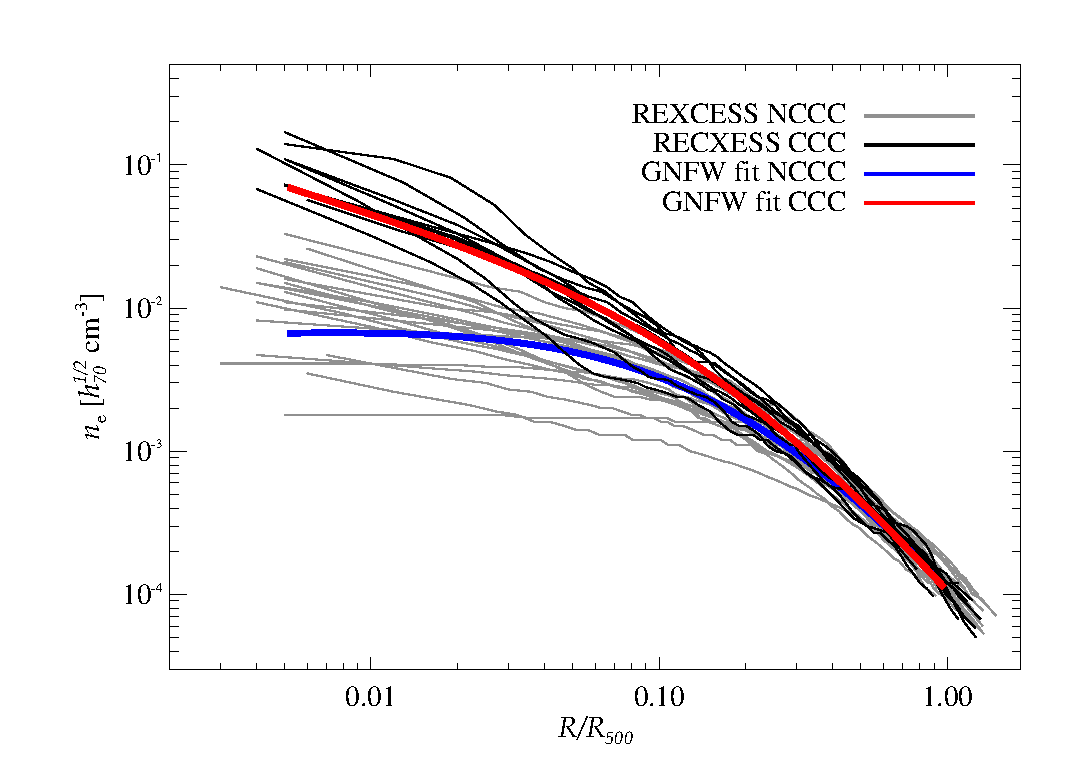
\includegraphics[width=0.5\textwidth]{figures/gas_profiles.eps}
\caption{Electron density profiles of the 31 clusters in the REXCESS sample. Grey and black lines represent NCCCs and CCCs, respectively. The blue and red lines represent our GNFW mean profile for the NCCCs and CCCs, respectively.}
\label{fig:gas_profiles}
\end{figure}

In order to obtain a general electron density profile that we will attach to our
simulated clusters, we use a generalized Navarro-Frank-White (GNFW) profile,
\begin{equation}
n_{\rmn{e}}(x) = \frac{n_{0}}{x^{\beta}\left[1+x^{\alpha}\right]^{\frac{\delta-\beta}{\alpha}}},
\label{eq:gnfw}
\end{equation}
where $x=R/R_{\rmn{c}}$ and $R_{\rmn{c}}$ is the cluster core radius. To reduce
the dimensionality of our fit, we fix representative values of $R_{\rmn{c}} =
0.2\, R_{500}$, $\alpha = 1$ and $\delta = 2.5$. We fit the REXCESS profiles in
log-log space, separating them in the two categories of NCCCs and CCCs as shown
in Figure~\ref{fig:gas_profiles}. The resulting fits are shown in blue and red
for the NCCC and CCC population, respectively. We obtain $n_{\rmn{0,NCCC}} =
1.02\times10^{-2}$~$h_{70}^{1/2}$~cm$^{-3}$, $n_{\rmn{0,CCC}} =
8.32\times10^{-3}$~$h_{70}^{1/2}$~cm$^{-3}$, $\beta_{\rmn{NCCC}} = -0.093$. and
$\beta_{\rmn{CCC}} = 0.592$.

The next step is to introduce a mass-scaling in order to apply our GNFW profiles
to all our clusters. We adopt a gas mass fraction-mass scaling,
$f_{gas,500}-M_{500}$ of \cite{2009ApJ...693.1142S} (and adopt their Equation~(8)). We can
express $f_{\rmn{gas},500}$ in the following way:
\begin{equation}
f_{\rmn{gas},500} = \frac{M_{\rmn{gas},500}}{M_{500}}  = \frac{\int_{0}^{R_{500}} \rho_{\rmn{gas}} \rmn{d}V}{M_{500}}
\label{eq:m500}
\end{equation}
with $\rho_{\rmn{gas}} = n_{\rmn{e}} m_{\rmn{p}} / ( X_{\rmn{H}}X_{\rmn{e}} )$ where
$m_{\rmn{p}}$ is the proton mass, $X_{\rmn{H}} = 0.76$ is the primordial hydrogen
mass fraction and $X_{\rmn{e}} = 1.157$ the ratio of electron-hydrogen number
densities in the fully ionized ICM \citep{1988xrec.book.....S}. For each cluster
$i$ of our sample, we then define a \emph{mass-scaled} gas profile as
$\rho_{\rmn{gas},i}=C_{i} \,\rho_{\rmn{gas}}$ with:
\begin{eqnarray}
%C_{i}  =  (0.0616\pm(0.0060g_{1}))  h_{73}^{-1.5}  \left(\frac{M_{500,i}}{10^{13} h_{73}^{-1} \rmn{M_{\odot}}}\right)^{0.135\pm(0.030g_{2})} \nonumber \\
C_{i}  & = &  (0.0656\pm(0.0064g_{1})) \, h_{70}^{-1.5}  \nonumber \\
 & \times & \left(\frac{M_{500,i}}{1.04 \times 10^{13} h_{70}^{-1} \rmn{M_{\odot}}}\right)^{0.135\pm(0.030g_{2})} \frac{M_{500,i}}{\int_{0}^{R_{500,i}} \rho_{\rmn{gas}} \rmn{d}V}
\label{eq:gas_scaling}
\end{eqnarray}
where $g_{1}$ and $g_{2}$ are random Gaussian number which we use in order to
simulate the natural scatter of the gas profiles.\footnote{The values
  $0.0064$ and $0.03$ quoted in Equation~(\ref{eq:gas_scaling}) do not represent
  the proper scatter of the $f_{\rmn{gas},500}-M_{500}$ relation but reflect the
  parameter errors and we rescaled the numerical values to a Hubble constant of
  $h_{70}$ used in this work.}

Hence, for each cluster in our sample we obtain a gas density profile
$\rho_{\rmn{gas},i}$ that obeys the observed $f_{gas,500}-M_{500}$ relation and
is uniquely determined by its DM mass $M_{500,i}$ and by the property of being a
NCCC or CCC. We assign the latter property to every halo depending on its
merging history. In particular, we make use of the offset parameter
$X_{\rmn{off}}$ computed for the MultiDark halo catalog. This is defined as the
ratio between the distance from the halo center to the center of mass and the
virial radius. The parameter assesses the dynamical state of the cluster and
whether the halo experienced a recent merger or not. Current observations reveal
a ratio of NCCCs and CCCs of about $50\%$ (see, e.g.~\citealp{2007A&A...466..805C,
  2009MNRAS.395..764S}). Since there is a correlation between merging clusters
and NCCCs, we use the median of the $X_{\rmn{off}}$ distribution to separate our
sample into CCCs and NCCCs (with NCCCs as those halos with the larger dynamical
offsets). Clearly, this is an over-simplification, and future X-ray surveys will
have to determine this property also as a function of redshift.

We also account for redshift evolution of the gas profiles. While our NCCC and
CCC gas profiles as derived from the REXCESS cluster sample are merely used to
define a profile shape, the normalization of the gas profiles is set by the
observational $f_{\rmn{gas},500}-M_{500}$ relation \citep{2009ApJ...693.1142S}.
The 43 clusters used in \cite{2009ApJ...693.1142S} have redshifts $0.012 < z <
0.12$ with a \emph{median} of $z \approx 0.04$. Thus, our phenomenological gas
profile is representative of the cluster population at $z=0$. To extend this
profile to high-$z$, we include a \emph{self-similar} scaling of the gas density
as $\rho_{\rmn{gas}}(z) = E(z)^{2} \rho_{\rmn{gas}}(z=0)$, where $E(z)^{2} =
\Omega_{\rmn{m}} (1+z)^{3} + \Omega_{{\Lambda}}$.


\subsection{X-ray and SZ scaling relations}
\label{sec:X-SZ-scaling}

In order to check whether our phenomenologically derived gas profiles reproduce
the observations, we calculate the bolometric X-ray thermal bremsstrahlung
luminosity $L_{\rmn{bol}}$ as in \cite{1988xrec.book.....S}\footnote{We check
  our procedure by fitting each of the 31 REXCESS clusters with
  equation~(\ref{eq:gnfw}) and calculating $L_{\rmn{bol}}$ with the measured gas
  temperature of each cluster. As a result, we fall short of the observed
  luminosity by a mean (median) of about $21\%$ ($20\%$). This is reasonable
  considering that we do not permit the parameters $R_{\rmn{c}}$, $\alpha$ and
  $\gamma$ to vary between different objects. Additionally, we neglect atomic
  line emission which may give a noticeable contribution, in particularly for
  low-mass clusters and in the cluster outskirts of larger systems.}  and
compare our sample result with the observed $L_{\rmn{bol}} - M_{500}$ relation
and XLF.\footnote{The mean (median) difference at $z=0$ between
  $L_{\rmn{bol}}$ within $R_{200}$ or within $R_{500}$ is $\approx 5\%$ ($\approx
  7\%$). While $L_{\rmn{bol}}$ refers to the quantity calculated within
  $R_{500}$, we note that the XLF for luminosities calculated within $R_{200}$
  will be barely changed.}

To assign a temperature to our model clusters (that is needed for calculating
$L_{\rmn{bol}}$ and $Y_{\rmn{X}}$), we adopt the $T-M_{500}$ relation by
\cite{2010MNRAS.406.1773M},
\begin{equation}
\log_{10} \left( \frac{k_{\rmn{B}}T_{\rmn{ci}}}{\rmn{keV}} \right) = 
A + B~\log_{10} \left( \frac{E(z) M_{500}}{10^{15} h_{70}^{-1} \rmn{M_{\odot}}} \right)
\label{eq:temp}
\end{equation}
where $A=0.91$, $B=0.46$, $T_{\rmn{ci}}$ is the cluster temperature \emph{not}
centrally excised (see \citealp{2010MNRAS.406.1773M}) and $k_{\rmn{B}}$ is the
Boltzmann constant. \cite{2010MNRAS.406.1773M} report a scatter of
$\sigma_{\rmn{yx}} = 0.06,$\footnote{Scatter is calculated as
  $\sigma_{\rmn{yx}} = \sqrt{ \left\{ \Sigma_{i=1}^{N} [Y_{i}-(A+B~X_{i})]^{2}\right\} /
    N-1}$ where the sum extends over the data points $X_{i}, Y_{i}$, and $A$ and $B$
  are the fit parameters.} which we apply to our sample using Gaussian
deviates.

In the left panel of Figure~\ref{fig:X_LM}, we show how our model
$L_{\rmn{bol}}-M_{500}$ relation compares with observations by
\cite{2010MNRAS.406.1773M} (\emph{all} data, see their Table~7). Their sample is
composed of 238 clusters at $0.02<z<0.46$ with a median of $z \approx 0.2$ and
self-consistently takes into account all selection effects, covariances,
systematic uncertainties and the cluster mass function. For this reason, we
compare the \cite{2010MNRAS.406.1773M} data to our model at $z=0.2$, and limit
the comparison to the mass range covered by the observations. Overall, there is
reassuring agreement between our phenomenological model and the data, which
probe our model most closely on scales around the cluster core radii (which is
where the contribution to $L_{\rmn{X}}$ per logarithmic interval in radius, $\dd
L_{\rmn{X}}/\dd\log r \propto r^3 n^2(r) \sqrt{k_{\rmn{B}}T}$, attains its maximum).  In
Table~\ref{tab:LMfits}, we show our model $L_{\rmn{bol}}-M_{500}$ scaling
relation and its scatter for different redshifts. We find that the scatter of
our samples at all redshifts are Gaussian distributed with a standard deviation
of $\sigma_{yx} \approx 0.18$ that matches the observational results of
\cite{2010MNRAS.406.1773M}, which report a scatter of $\sigma_{yx} = 0.185$.

\begin{figure*}[t]
\centering
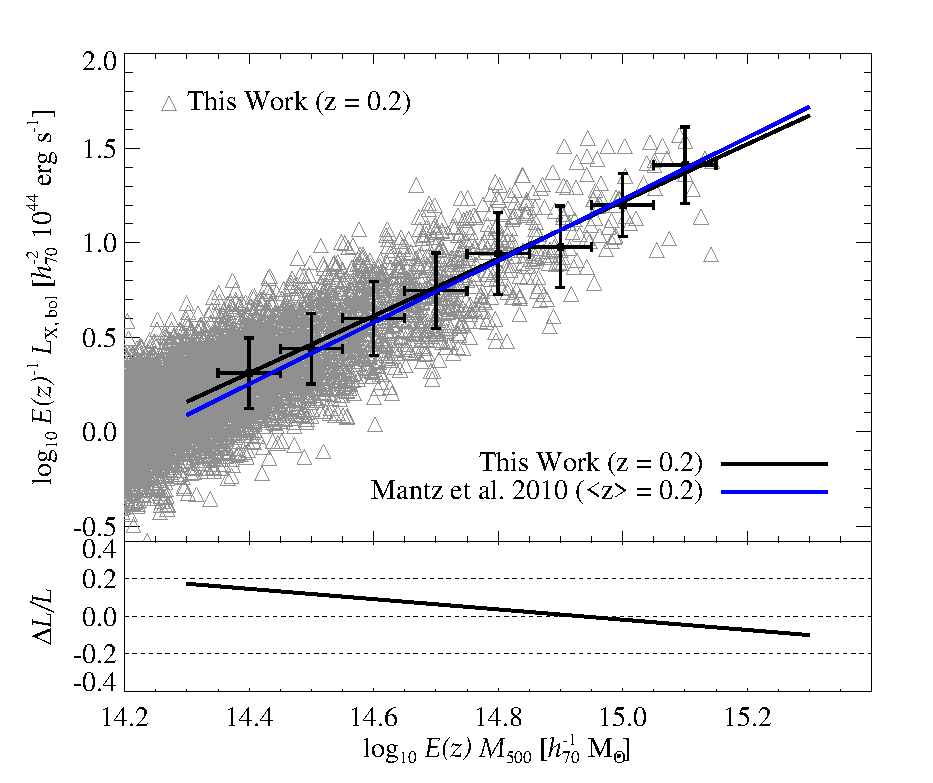
\includegraphics[width=0.33\textwidth]{figures/lx_m.eps}
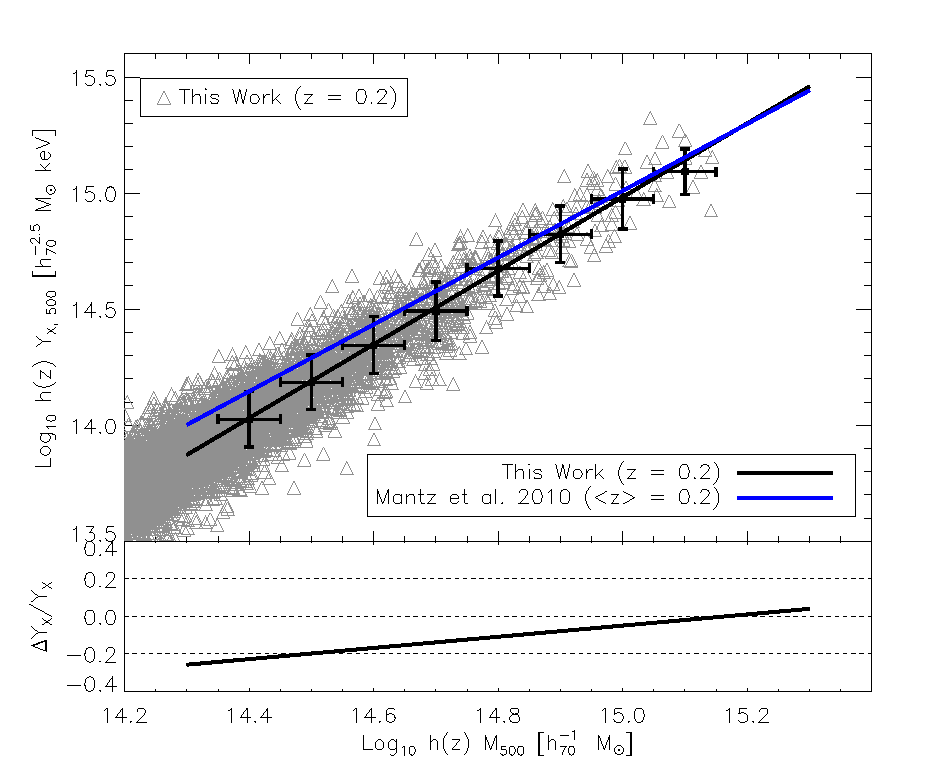
\includegraphics[width=0.33\textwidth]{figures/yx_m.eps}
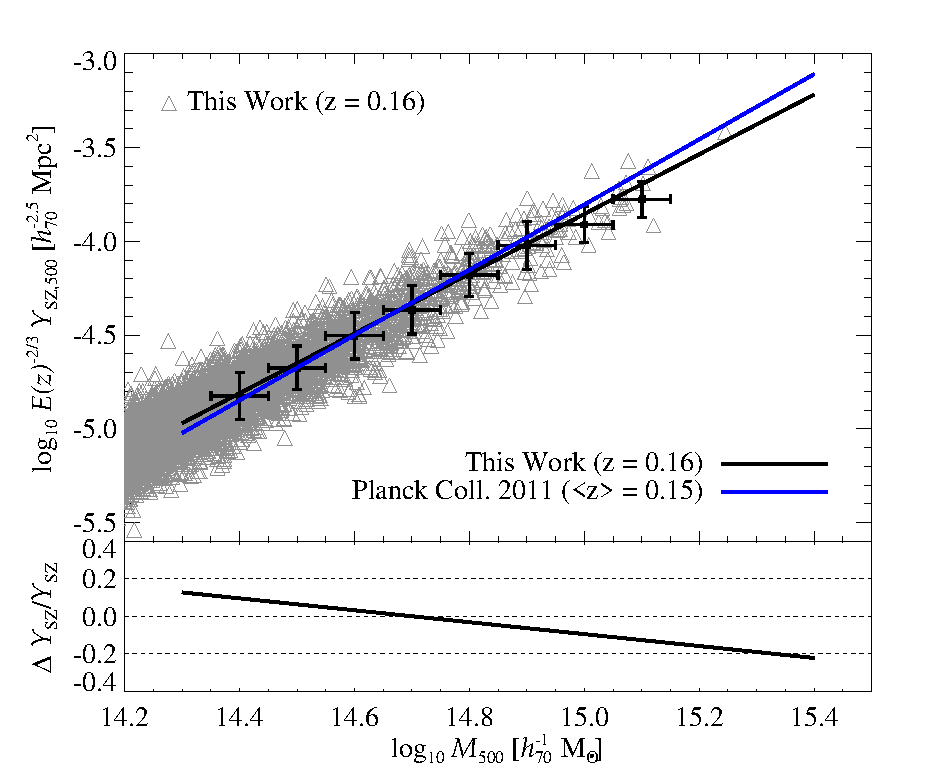
\includegraphics[width=0.33\textwidth]{figures/sz_m.eps}
\caption{X-ray and SZ scaling relations. Grey triangles show the MultiDark
  sample (limited to the mass range covered by observations), the black line is
  the corresponding scaling relation, and the blue line is the
  observational result. The black crosses represent the median values of the
  quantity in question for a given mass bin (indicated by horizontal error
  bars), and the vertical error bars represent the standard deviation within a
  bin.  \emph{Left.} We compare the bolometric X-ray luminosity-to-mass
  relation, $L_{\rmn{bol}}-M_{500}$, at $z=0.2$ to the observational sample by
  \cite{2010MNRAS.406.1773M} with a median of $z \approx 0.2$. \emph{Center.}
  $Y_{\rmn{X}}-M_{500}$ scaling relation of our model in comparison to the
  observational sample by \cite{2010MNRAS.406.1773M}. \emph{Right.}
  $Y_{\rmn{SZ}}-M_{500}$ scaling relation at $z=0.16$ in comparison
  to the observational sample by \cite{2011A&A...536A..11P} with a median
  redshift of about $0.15$. The bottom panels show the relative difference to
  the observational scaling relations. 
  }
\label{fig:X_LM}
\end{figure*}

\begin{table}[t]
\begin{center}
\caption{$L_{\rmn{bol}}-M_{500}$ Scaling Relations.}
\medskip
\begin{tabular}{cccc}
\hline
\phantom{\Big|}
Redshift $z$ & $A$ & $B$ & $\sigma_{yx}$ \\
\hline \\[-0.5em]
 0      & $-21.41\pm0.11$ & $1.50\pm0.01$ & 0.179\\
 0.1   & $-21.30\pm0.12$ & $1.50\pm0.01$ & 0.179\\
 0.2   & $-21.50\pm0.13$ & $1.51\pm0.01$ & 0.178\\ 
 0.4   & $-21.13\pm0.17$ & $1.49\pm0.01$ & 0.178\\ 
 0.61 & $-21.59\pm0.22$ & $1.53\pm0.01$ & 0.177\\ 
 0.78 & $-20.73\pm0.29$ & $1.48\pm0.02$ & 0.177\\ 
 1      & $-20.45\pm0.42$ & $1.46\pm0.03$ & 0.177\\[0.5em]
\hline
\end{tabular}
\label{tab:LMfits}
\end{center}
\footnotesize{Note. Scaling relations are reported in the form of $\log_{10}~(L_{\rmn{bol}}~/~E(z)~h_{70}^{-2}~10^{44}~\rmn{erg~s}^{-1})=A+B~\log_{10}~(E(z)~M_{500}~/~h_{70}^{-1}~\rmn{M_{\odot}})$. The relation scatter $\sigma_{yx}$ is also shown.}
\end{table}

In the middle panel of Figure~\ref{fig:X_LM}, we compare the
$Y_{\rmn{X}}-M_{500}$ relation of our sample to observational data
\citep{2010MNRAS.406.1773M}. The model agrees nicely at high-mass end, but
underpredicts the observed scaling at low masses by about $20\%$ (at the
1-$\sigma$ level). This is the same level of deviations from the data as in the
case of $L_{\rmn{X}}$, which is more significant due to the smaller scatter in
the $Y_{\rmn{X}}$ relation. The differential contribution to the thermal energy
per logarithmic interval in radius (and hence to the integrated Compton-$y$
parameter) is given by $\dd Y /\dd\log r \propto r^3 P_{\rmn{th}}(r)$, with the
thermal gas pressure $P_{\rmn{th}}=n_{\rmn{gas}}k_{\rmn{B}}T$. It peaks at
scales slightly smaller than $R_{500}$ with 1-$\sigma$ contributions extending
out to $3\,R_{500}$ \citep{2010ApJ...725...91B}. Hence, the observational
scaling constrains our model on those large scales, quite complementary to the
X-ray luminosity. The deviations at small masses either indicates different
assumptions about $f_{\rmn{gas}}$, the gas temperature, or different selection
effects of either observational sample that we used to calibrate our model or to
compare out scaling relation to. E.g., \cite{2010MNRAS.406.1773M} determine
their masses by adopting a constant value for $f_{\rmn{gas}}$, in contrast to
our approach which adopts the observed $f_{\rmn{gas},500}-M_{500}$ relation
given by \cite{2009ApJ...693.1142S}. Additionally, we adopt the \emph{centrally
  included} temperature \cite{2010MNRAS.406.1773M} throughout all our work,
while \cite{2010MNRAS.406.1773M} use the \emph{centrally excised} temperature to
calculate $Y_{\rmn{X}}$. This assumption also impacts the scatter of the
$Y_{\rmn{X}}-M$ relation. In fact, using the \emph{centrally included}
temperature, we found a scatter of $\sigma_{yx} \approx 0.11$ (see
Table~\ref{tab:YXfits} where our $Y_{\rmn{X}}$ scaling relations are reported),
significantly higher than the value of $\sigma_{yx} = 0.052$ found by
\cite{2010MNRAS.406.1773M}.

In the right panel of Figure~\ref{fig:X_LM}, we compare the
$Y_{\rmn{SZ}}-M_{500}$ relation in our model (calculated as in Equation~(3) of
\citealp{2011arXiv1109.3709B}) with the observed scaling relation by
\cite{2011A&A...536A..11P}. Their sample contains clusters up to $z \approx
0.45$ and has a median of $z \approx 0.15$; hence, we compare the data to our
relation at the MultiDark snapshot $z=0.16$ (containing 11419 clusters above our
mass cut) which however is not used throughout the rest of the work. Our model
reproduces the data remarkably well, except for the high-mass end where our
simulations have a weaker constraining power due to the comparably small box
size in comparison to the survey volume of {\em Planck}. In
Table~\ref{tab:YSZfits}, we report our SZ scaling relations for different
redshifts. We find a scatter of $\sigma_{yx} \approx 0.11$ which compares well
with the \emph{Planck} result of $\sigma_{yx} \approx 0.1$.
 
\begin{table}[t]
\begin{center}
\caption{$Y_{\rmn{X}, 500}-M_{500}$ Scaling Relations.}
\medskip
\begin{tabular}{cccc}
\hline
\phantom{\Big|}
Redshift $z$ & $A$ & $B$ & $\sigma_{yx}$ \\
\hline\\[-0.5em]
 0      & $-9.18\pm0.07$ & $1.61\pm0.01$ & 0.109\\
 0.1   & $-8.85\pm0.07$ & $1.59\pm0.01$ & 0.109\\
 0.2   & $-8.82\pm0.08$ & $1.59\pm0.01$ & 0.109\\ 
 0.4   & $-8.79\pm0.10$ & $1.59\pm0.01$ & 0.108\\ 
 0.61 & $-8.65\pm0.14$ & $1.59\pm0.01$ & 0.109\\ 
 0.78 & $-8.36\pm0.18$ & $1.57\pm0.01$ & 0.109\\ 
 1      & $-8.28\pm0.26$ & $1.57\pm0.02$ & 0.109\\[0.5em]  
\hline
\end{tabular}
\label{tab:YXfits}
\end{center}
\footnotesize{Note. Scaling relations are reported in the form of $\log_{10}~(E(z)~Y_{\rmn{X},500}~/~h_{70}^{-2.5}~\rmn{M_{\odot}}~\rmn{keV})=A+B~\log_{10}~(E(z)~M_{500}~/~h_{70}^{-1}~\rmn{M_{\odot}})$. The relation scatter $\sigma_{yx}$ is also shown.}
\end{table}

\begin{table}[t]
\begin{center}
\caption{$Y_{\rmn{SZ}, 500}-M_{500}$ Scaling Relations.}
\medskip
\begin{tabular}{cccc}
\hline
\phantom{\Big|}
Redshift $z$ & $A$ & $B$ & $\sigma_{yx}$ \\
\hline\\[-0.5em]
 0      & $-27.93\pm0.07$ & $1.60\pm0.01$ & 0.109\\
 0.1   & $-27.74\pm0.07$ & $1.59\pm0.01$ & 0.109\\
 0.16 & $-27.76\pm0.08$ & $1.59\pm0.01$ & 0.109\\
 0.2   & $-27.65\pm0.08$ & $1.59\pm0.01$ & 0.109\\ 
 0.4   & $-27.57\pm0.10$ & $1.59\pm0.01$ & 0.108\\ 
 0.61 & $-27.50\pm0.13$ & $1.59\pm0.01$ & 0.109\\ 
 0.78 & $-27.15\pm0.18$ & $1.58\pm0.01$ & 0.109\\ 
 1      & $-27.01\pm0.26$ & $1.58\pm0.02$ & 0.109\\[0.5em] 
\hline
\end{tabular}
\label{tab:YSZfits}
\end{center}
\footnotesize{Note. Scaling relations are reported in the form of $\log_{10}~(E(z)^{-2/3}~Y_{\rmn{SZ},500}~/~h_{70}^{-2.5}~\rmn{Mpc}^{2})=A+B~\log_{10}~(E(z)~M_{500}~/~h_{70}^{-1}~\rmn{M_{\odot}})$. The relation scatter $\sigma_{yx}$ is also shown.}
\end{table}



\subsection{X-ray luminosity function}

The XLF study has been somehow abandoned during the last years due to the
difficulties of using the X-ray luminosity for cosmological purposes. The X-ray
emissivity scales with the square of the gas density, which makes it subject to
density variations and clumping. This implies large scatter that causes a large
Malmquist bias and underlines the necessity of careful mock surveys that need to
address all systematics.

Nevertheless, it provides a complementary check for our model. To this end, we
use the \emph{ROSAT} brightest cluster sample (BCS) XLF
\citep{1997ApJ...479L.101E}, which is in good agreement with results from the
ROSAT ESO Flux-Limited X-ray (REFLEX; \citealp{2002ApJ...566...93B}) and
HIFLUGCS \citep{2002ApJ...567..716R}.  Note that the XLF is fully determined by
the mass function and the $L_{\rmn{X}}-M_{500}$ relation after taking into
account the observational biases. This means that applying the Malmquist bias
corrected $L_{\rmn{X}}-M_{500}$ relation by \cite{2010MNRAS.406.1773M} directly
to the MultiDark mass function and accounting for the observational scatter in
$L_{\rmn{X}}-M_{500}$ should yield an unbiased XLF. We show the resulting
bolometric and soft-band ($0.1-2.4$~keV) XLF in Figure~\ref{fig:XLF} and compare
those to the corresponding BCS XLFs (for which bolometric band there is only the 
Schechter fit available) and to our model predictions.  While the soft-band XLF by
\cite{2010MNRAS.406.1773M} agrees well with the BCS data points, it deviates
from the corresponding Schechter fit at low luminosities. This is also true in
the bolometric band, where the XLFs of \cite{2010MNRAS.406.1773M} and our model
agree well, but deviate from the BCS Schechter fit at low luminosities. This may
be an artifact due to the use of Schechter fit instead of the data points or may
point to incompleteness of the BCS sample. Note that the Poissonian errors of
the XLF obtained from the MultiDark simulation are a lower limit as we are
neglecting the uncertainty due to cosmic variance.  Studies of the XLF will
become again an important topic with the upcoming launch of the eROSITA
satellite (see e.g.~\citealp{2011MSAIS..17..159C}) and further studies in this
direction are desirable. For these reasons, we do not show XLF predictions at
other redshifts, leaving this for a future study (Zandanel et al., in prep.).

\begin{figure}[t]
\centering
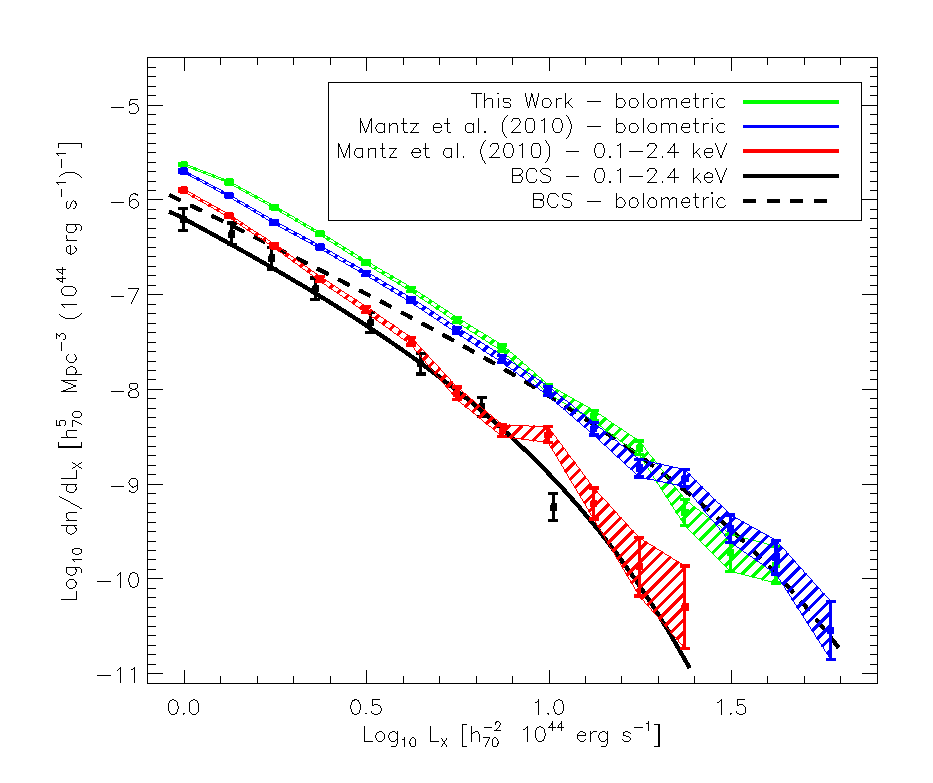
\includegraphics[width=0.48\textwidth]{figures/xlf.eps}
\caption{Bolometric and soft-band ($0.1-2.4$~keV) XLFs. Shown are the soft-band
  data points, the soft-band and bolometric Schechter fits of the BCS sample of
  \cite{1997ApJ...479L.101E}, which has a median of $z \approx 0.08$.  While the
  soft-band XLF of \cite{2010MNRAS.406.1773M} compares well with the BCS data
  points, it deviates from the corresponding Schechter fit. We also show the
  bolometric XLF of \cite{2010MNRAS.406.1773M} and bolometric XLF of our model at
  $z=0.1$. The XLFs are calculated in equally log-spaced mass bins; the error
  bars represent the Poissonian errors. Note that we limit the comparison to the
  luminosity range covered by our sample, where we cut the lowest part because
  in that range the XLF rapidly drops due to the imposed mass cut.  }
\label{fig:XLF}
\end{figure}

Summarizing, our phenomenological approach provides viable gas densities that
reproduce the observed scaling relations of the ICM as well as the XLF. Thus, we
will apply it in the following to model the CR population in galaxy clusters and
to predict the radio and gamma-ray emission of our sample.


%%%%%%%%%%%%%%%%%%%%%%%%%%%%%%%%%%%%%%%%%%%%%%%%%%%%%%%%%%%%%%%%%%%
\subsection{Cosmic ray modeling}
\label{sec:2.3}
We assume a power-law CR proton distribution, $f(p) \dd p=C p^\alpha \dd p$,
which is the effective one-dimensional momentum distribution (assuming isotropy
in momentum space). We are interested in calculating the radio synchrotron (and
gamma-ray) emission resulting from secondaries of hadronic CR interactions with
protons of the ICM. To start, we provide the synchrotron emissivity $j_{\nu}$ at
frequency $\nu$ and per steradian of a steady-state electron population where
radiative cooling balances injection from hadronic interactions (adapted from
\citealp{2008MNRAS.385.1211P} and \citealp{2011A&A...527A..99E}),
\begin{equation}
j_{\nu}  =  A_\nu C(R) \rho_{\rmn{gas}}(R) 
\frac{\epsilon_{\rmn{B}}(R)}{\epsilon_{\rmn{B}}(R)+\epsilon_{\rmn{CMB}}} 
\left( \frac{\epsilon_{\rmn{B}}(R)}{\epsilon_{B_{\rmn{c}}}} \right)^{(\alpha-2)/4},
\label{eq:jnu}
\end{equation}
where the abbreviations $A_\nu$ and $\epsilon_{B_{\rmn{c}}}$ are defined in
Appendix~\ref{app:A}, $\epsilon_{\rmn{CMB}}$ is the energy density of the cosmic
microwave background (CMB), and $\epsilon_B=B^{2}/(8\pi)$ denotes the magnetic
energy density. We assume a scaling of the magnetic field with gas density that
is given by
\begin{equation}
B(R) = B_0\,\left(\frac{\rho_{\rmn{gas}}(R)}{\rho_{\rmn{gas},0}}\right)^{\alpha_B},
\label{eq:B}
\end{equation}
where $B_0$ is the central magnetic field and $\alpha_{\rmn{B}}$ a parameter
representing the rate of decline of the magnetic field strength toward the
cluster outskirts. The radio surface brightness $S_{\nu}(R_{\perp})$ (in the small
angles approximation) and luminosity $L_{\nu}$ at a given frequency $\nu$ are given by
\begin{eqnarray}
S(R_{\perp}) &=& 2 \int_{R_{\perp}}^{\infty} j_{\nu}(R) \frac{R}{\sqrt{R^{2}-R_{\perp}^{2}}} \rmn{d}R, \label{eq:surf} \\
L_{\nu}  &=&  4 \pi \int \dd V j_\nu(R).
\label{eq:lum}
\end{eqnarray}
The flux is given by $F_{\nu}=L_{\nu}/(4\pi D^{2})$ where $D$ is the
luminosity distance of the considered object. Note that we do not
include any convolution with instrumental point spread functions 
unless differently specified.

The spatial CR distribution within galaxy clusters is governed by an interplay
of advection, CR streaming and diffusion. The advection of CRs by turbulent gas
motions is dominated by the largest eddy turnover time $\tau_{\rmn{tu}}\sim
L_{\rmn{tu}}/ \vel_{\rmn{tu}}$, where $L_{\rmn{tu}}$ denotes the turbulent
injection scale (typically of order the core radius) and $\vel_{\rmn{tu}}$ the
associated turbulent velocity that gets close to the sound speed
$\vel_{\rmn{s}}$ for transsonic turbulence after a cluster merger and relaxes to
small velocities afterwards. In contrast, the crossing time of streaming CRs
over $L_{\rmn{tu}}$ is $\tau_{\rmn{st}}\sim \chi_B\,L_{\rmn{tu}}/
\vel_{\rmn{st}}$ with the streaming velocity given by $\vel_{\rmn{st}}\sim
\vel_{\rmn{s}}$ and $\chi_B\lesssim 1$ parametrizes the magnetic bending scale
and hence magnetic bottlenecks for the macroscopic, diffusive CR transport,
which are critical in lowering the microscopic streaming velocity of CR by some
finite factor. Hence, we can define a turbulent propagation parameter
$\gamma_{\rmn{tu}}\equiv \tau_{\rmn{st}}/\tau_{\rmn{tu}}$ that indicates the
relative importance of advection versus CR streaming as the dominant CR
transport mechanism. After a merger, turbulent advective transport dominates
yielding $\gamma_{\rmn{tu}}\gg 1$ which results in centrally enhanced CR
profiles. In contrast, in a relaxed cluster, CR streaming should be the dominant
transport mechanism implying $\gamma_{\rmn{tu}}\sim1$ and producing flat CR
profiles (for a detailed discussion of these processes, see
\citealp{2011A&A...527A..99E}).

What we propose here is to keep the spectral shape of the CR distribution
function as determined from cosmological hydrodynamical simulation of clusters
\citep{2010MNRAS.409..449P} that however did not account for CR streaming. Hence
the spatial CR distribution has to be modified to include effects of CR
streaming and use the analytical result from \citet{2011A&A...527A..99E}. In
that way we want to obtain a model that includes the necessary CR transport
physics and is able to predict the radio and gamma-ray emission and to reproduce
the main observed RH properties.  Note that this approach is not fully
self-consistent and points to the necessity of future hydrodynamical simulations
to include the effect of CR streaming and diffusion on the CR spectrum.

\begin{figure*}[t]
\centering
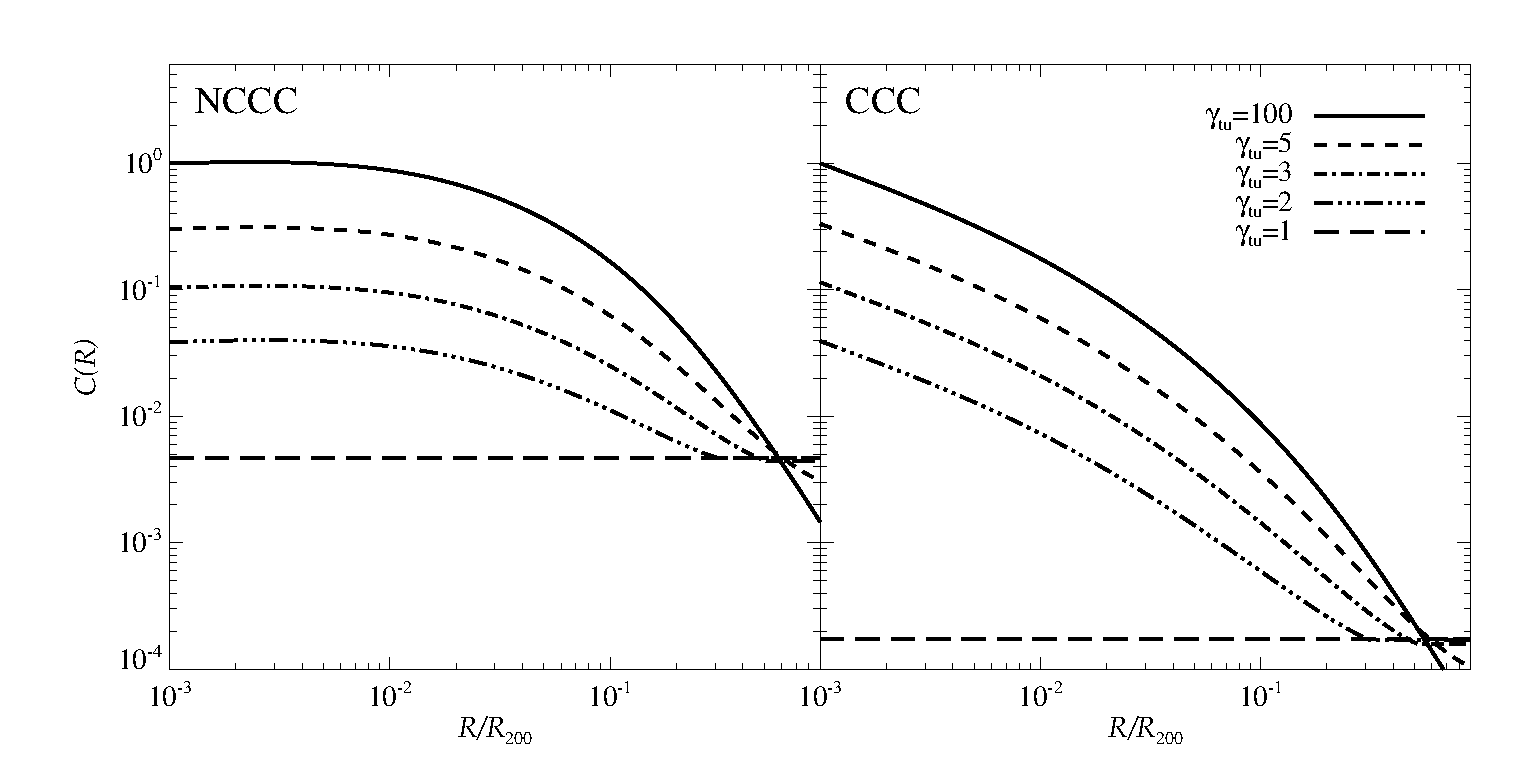
\includegraphics[width=0.62\textwidth]{figures/CR_profiles_FinalModel.eps}
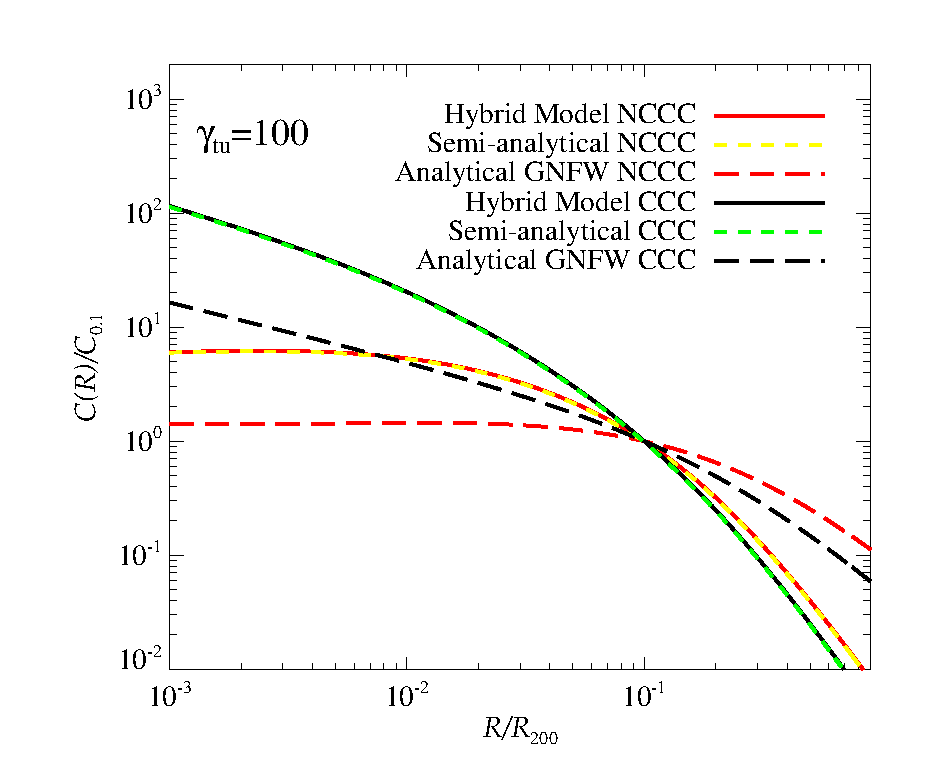
\includegraphics[width=0.37\textwidth]{figures/CR_profiles_FinalModelvsREX_norm0.1.eps}
\caption{Left panel: we show our final hybrid model profile for the normalization of
  the CR distribution for the NCCC and CCC cases and for
  different values of $\gamma_{\rmn{tu}}$. We normalize $C$ by
  requiring the CR populations to have a constant total CR number within
  $R_{200}$. Right panel: we compare the hybrid model (adopting $\gamma_{\rmn{tu}}=100$) with the semi-analytical
  advection-only case (adopting our GNFW gas profiles and the outer temperature
  decrease to the simulation-derived model proposed by
  \citealp{2010MNRAS.409..449P}) and with the exact analytical solution as in
  \citet{2011A&A...527A..99E}, but for our GNFW profiles (adopting $\alpha=2.3$
  and $\gamma_{\rmn{tu}}=100$). Here, the CR profiles are normalized at
  $C_{0.1}=C(0.1R_{200})$.}
\label{fig:CRFinalModel}
\end{figure*}

To construct such a model, we have to generalize the approach by
\citet{2011A&A...527A..99E} in order to account for GNFW gas profiles
(Section~\ref{sec:2.2}) and to include the mass-scaling of the CR normalization
obtained from simulations \citep{2010MNRAS.409..449P}. While details are given
in Appendix~\ref{app:B}, we show the main steps here. When turbulent advection
completely dominates the CR transport, the CR normalization can be written
\citep{2011A&A...527A..99E}
\begin{equation}
C_{\rmn{adv}}(R)=C_{0} \left( \frac{P_{\rmn{th}}(R)}{P_{\rmn{th},0}} \right)^{\frac{\beta_{\rmn{CR}}}{\gamma}} = 
C_{0} \eta(R)^{\beta_{\rmn{CR}}},
\label{eq:Csimple_1}
\end{equation} 
where $\beta_{\rmn{CR}}=(\alpha+2)/3$, $\gamma=5/3$, and 
we introduced the advective CR profile $\eta(R)=(P(R)/P_0)^{1/\gamma}$. 
Solving the continuity equation for CRs, \citet{2011A&A...527A..99E} derive the CR density profile,
\begin{equation}
\rho_{\rmn{CR}}(R) = \rho_{\rmn{CR},0} \eta(R) \rmn{exp} \left( \frac{R}{R_{*}} \right) \, ,
\label{eg:rhoCR_1}
\end{equation} 
where $R_{*}=\gamma_{\rmn{\rmn{tu}}}R_{\rmn{c}}$ and $R_{\rmn{c}}$ is the characteristic 
radius, of order the core radius, at which the turbulence is supposed to be injected.
Now, we introduce the \emph{semi-analytical} mass-dependent normalization of the
CR profile of \cite{2010MNRAS.409..449P} such that
\begin{equation}
\eta(R) = \left( \frac{C_{\rmn{adv}}(R)}{C_0} \right)^{1/\beta_{\rmn{CR}}} = 
\left( \frac{C_{\rmn{hybrid}}(R)}{C_0} \right)^{1/\beta_{\rmn{CR}}} \, ,
\label{eq:eta}
\end{equation} 
which effectively redefines $C_{\rmn{adv}}(R)$ by the CR normalization in our hybrid model,
\begin{equation}
C_{\rmn{hybrid}}(R) =  \tilde{C}(R)\, \frac{\rho_{\rmn{gas}}(R)}{m_\rmn{p}} \frac{T(R)}{T_0}.
\label{eq:Cf}
\end{equation} 
Here, $\tilde{C}(R)$ is the normalization CR profile of Equation~(22) of
\cite{2010MNRAS.409..449P} and we additionally account for the temperature decline toward
the cluster periphery, $T(R)$, expected by the fit to the universal temperature profile
derived from cosmological cluster simulations
\citep{2007MNRAS.378..385P,2010MNRAS.409..449P} and deep {\em Chandra} X-ray
observations \citep{2005ApJ...628..655V}. Eventually, our final hybrid CR
normalization is $C(R)=C_{0}(\rho_{\rmn{CR}}(R)/\rho_{\rmn{CR},0})^{\beta_{\rmn{CR}}}$
within $R_{\pm}$ of Equation~(\ref{eq:Rpm}), and $C(R) = C(R_{\pm})$ for $R > R_{+}$ 
and $R < R_{-}$, respectively.

The last step is to generalize the case of one CR population with a single
spectral index $\alpha$ to include spectral curvature as suggested by
\cite{2010MNRAS.409..449P} who model the CR spectrum with three different
power-law CR populations with spectral indices of
$\alpha_{i}=(2.15,2.3,2.55)$. Our presented formalism can be easily extended to
account for multiple CR populations by extending the terms with a single
$\alpha$ to sums over the three spectral indices (see
\citealp{2010MNRAS.409..449P}). This extension has to be applied to $A_{\nu}$,
to the factor $(\epsilon_{\rmn{B}}(R)/ \epsilon_{B_{\rmn{c}}})^{(\alpha-2)/4}$
of Equation~(\ref{eq:jnu}), and to Equation~(\ref{eq:Csimple_1}). While the
modifications are straight forward in the first two cases (and are adopted for
our hybrid model, see Appendix~\ref{app:A}), introducing a sum over $\alpha_{i}$
in Equation~(\ref{eq:Csimple_1}) would make impossible to analytically solve for
$\eta(R)$ in Equation~(\ref{eq:eta}). For simplicity, we decided to only use
$\alpha = 2.3$ in this last case.\footnote{We checked that
  the choice of $\alpha$ in Equation~(\ref{eq:Csimple_1}) has only a minor
  effect on the results. Varying $\alpha$ within $2.15-2.55$ leaves the radial
  shape and the normalization unchanged within $0.5\%$.} For the highly
turbulent cases, i.e., for $\gamma_{\rmn{tu}}=100$ (1000), we recover the radial
shape and normalization of the semi-analytical model of
\cite{2010MNRAS.409..449P} within $1\%$ ($0.1\%$).

Our final model for the CR distribution function, has the following properties:
(i) it accounts for X-ray-inferred (CCC and NCCC) gas profiles and cluster-mass
scalings of the gas fraction, in addition to the universal temperature drop in
the outskirts of clusters, (ii) a cluster-mass dependent CR normalization and
universal CR spectrum as derived from cosmological hydrodynamical cluster
simulations, (iii) an effective parametrization of active CR transport
processes, including CR streaming and diffusion, which allows us to explore
different turbulent states of the clusters in our MultiDark sample.

In the left panel of Figure~\ref{fig:CRFinalModel}, we show our final hybrid CR 
normalization for the NCCC and CCC cases and for different values of $\gamma_{\rmn{tu}}$. 
As expected, effective CR streaming (i.e., negligible advective turbulent transport
or equivalently, $\gamma_{\rmn{tu}}\sim1$) flattens the spatial CR profiles
irrespective of the the cluster state. Additionally, in the right panel, we
compare our final hybrid model profile with the
semi-analytical advection-only case (adopting our GNFW gas profiles and the
outer temperature decrease to the model proposed by \citealp{2010MNRAS.409..449P})
and with the exact analytical solution as in \citet{2011A&A...527A..99E}, but
for our GNFW profiles (adopting $\alpha=2.3$ and $\gamma_{\rmn{tu}}=100$, see
Appendix~\ref{app:B} for details).  The profiles are normalized at $0.1 R_{200}$. 
The main differences between our final model (and the semi-analytical
model) on the one side and the analytical solution on the other side is the
inclusion of the simulation-based ``reference'' profile $\tilde{C}$ for the
advection-only case and the universally observed temperature drop towards the
outskirts of clusters in our hybrid model. Note that our final model profiles
are generally more centrally peaked in comparison to the analytical GNFW case,
which is due to the enhanced radiative cooling in the \citet{2010MNRAS.409..449P} 
simulations that did not account for AGN feedback. Thanks to the
flexible parametrization in our model, this can be easily counteracted by
changing $\gamma_{\rmn{tu}}$ and $\alpha_B$, however, at the expense that these
parameters are now degenerate with our assumptions about the CR profile in the
advection-dominated regime and other possible effects that we are not considering 
here as e.g.~cluster asphericity (see also next Section~\ref{sec:3}).


%%%%%%%%%%%%%%%%%%%%%%%%%%%%%%%%%%%%%%%%%%%%%%%%%%%%%%%%%%%%%%%%%%%
%%%%%%%%%%%%%%%%%%%%%%%%%%%%%%%%%%%%%%%%%%%%%%%%%%%%%%%%%%%%%%%%%%%
\section{Radio Surface Brightness Modeling}
\label{sec:3}

In this Section we apply our model to reproduce the emission characteristics of
four well-observed RHs. Hence for the purpose of this section, we adopt the
measured gas and temperature profiles derived from X-ray observations of each cluster.  Our
final model includes an overall normalization $g_{\rmn{CR}}$ of the CR
distribution function and the hadronically-induced non-thermal emission 
%and can
%be included by substituting $A_{\nu}$ with
%$A_{\nu,\rmn{hybrid}}=g_{\rmn{CR}}A_{\nu}$ 
(see Appendix~\ref{app:A}). Note that
this parameter can be interpreted as a functional that depends on the
\emph{maximum CR acceleration efficiency}, $g(\zeta_{\rmn{p,max}})$,
\citep{2010MNRAS.409..449P} but \emph{only} for
$\gamma_{\rmn{tu}}\gtrsim100$. We will additionally study the CR-to-thermal
pressure $X_{\rmn{CR}}=P_{\rmn{CR}}/P_{\rmn{th}}$, where the CR pressure is
given by
\begin{equation}
  \label{eq:PCR}
  P_{\rmn{CR}}=\frac{g_{\rmn{CR}} C m_{\rmn{p}} c^{2}}{6}
  \sum_{i=1}^{3} \Delta_{i} \mathcal{B}_{1/(1+q^2)} \left(
    \frac{\alpha_{i}-1}{2},\frac{3-\alpha_{i}}{2} \right).
\end{equation}
Here, $c$ is the speed of light, $q=0.8$, and the normalization factors of the
individual CR populations are given by $\Delta_{i} = (0.767, 0.143, 0.0975)$
\citep[][see also Appendix~\ref{app:A}]{2010MNRAS.409..449P}. 


\subsection{Modelling individual radio halos}

For our study, we choose the giant radio halos of Coma
\citep{1997A&A...321...55D} and Abell~2163
\citep{2001A&A...373..106F,2009A&A...499..679M}, both merging NCCCs, and the
radio-mini halos of Perseus \citep{1990MNRAS.246..477P} and Ophiuchus
\citep{2009A&A...499..371G,2009A&A...499..679M}, both relaxed CCCs. The radio
emission of these clusters is representative of a wide class of RHs.
Additionally, Perseus, Ophiuchus and Coma are among the most promising clusters
for gamma-ray observations \citep{2010MNRAS.409..449P,2011arXiv1105.3240P}. In
Table~\ref{tab:RadioHalos}, we summarize the main characteristics of these halos
and detail the main parameters adopted for the modeling and the corresponding
results. In Figure~\ref{fig:SBmodeling}, we show the surface brightness and
CR-to-thermal pressure profile of each cluster. Note that we model these
clusters at 1.4~GHz and within $R_{200}$.

\begin{table*}[t]
\begin{center}
\caption{Radio Halos and Mini-Halos Characteristics.}
\medskip
%\begin{tabular}{c|c|c|c|c|c|c}
\begin{tabular}{cccccccc}
\hline
\phantom{\Big|}
name & $z$ & $D$ & $\Delta d$ & $L_{1.4~\rmn{GHz},~\rmn{obs}}$ & fit parameters & $L_{1.4~\rmn{GHz},~\rmn{model}}$ & references \\
\phantom{\Big|}
           &   & [$h_{70}^{-1}$~Mpc] & [$h_{70}^{-1}$~Mpc] & $10^{31}$ [$h_{70}^{-2}$~erg~s$^{-1}$~Hz$^{-1}$] & $\gamma_{\rmn{tu}}$, $\alpha_{\rmn{B}}$ & $10^{31}$ [$h_{70}^{-2}$~erg~s$^{-1}$~Hz$^{-1}$] & \\
\hline \\[-0.5em]
Coma           & $0.023$ & $101$ & $2.15$ & $0.72$  & 1, 0.6  & 0.86 &  [1, 2, 3]   \\
               &         &       &        &                        & 4, 0.3  & 0.90  &  \\
A~2163         & $0.203$ & $962$ & $2.07$ & $15.36$     & 1, 0.3  & 13.43  &  [3, 4]  \\
\hline \\[-0.5em]
Perseus        & $0.018$ & $78$   & $0.15$ & $4.40$ & 3, 0.4   & 4.80 &  [3, 5, 6]  \\
               &         &        &        &                       & 100, 0.3 & 3.97 &  \\
Ophiuchucs     & $0.028$ & $121$  & $0.41$ & $0.19$       & 5, 0.7   & 0.19  &  [3, 4] \\
               &         &        &        &                       & 100, 0.3 & 0.23 &   \\[0.5em]
\hline
\end{tabular}
\label{tab:RadioHalos}
\end{center}
\footnotesize{Note. Top two rows correspond to giant radio halos, while the
  bottom two rows are radio mini-halos. $\Delta d$ represents the approximate
  diameter of the RHs. $L_{1.4~\rmn{GHz},~\rmn{obs}}$ is the total luminosity at
  1.4~GHz. $M_{200}$ and $R_{200}$ are taken from \cite{2002ApJ...567..716R}. We
  use X-ray-inferred gas densities $\rho_{\rmn{gas}}$ and temperatures for Coma
  \citep{1992A&A...259L..31B}, for A~2163 and Ophiuchus
  \citep{2002ApJ...567..716R}, and for Perseus \citep{2003ApJ...590..225C}. For
  all clusters, we also adopt the outer temperature decrease seen in
  cosmological cluster simulations \citep[e.g.,][]{2010MNRAS.409..449P} and deep
  {\em Chandra} X-ray observations \citep{2005ApJ...628..655V}. Note that
  despite the fact that Ophiuchus is a CCC with a central temperature dip, we
  adopt a constant central temperature profile because the dip is only important
  below $30$~$h_{70}^{-1}$~kpc (see \citealp{2010MNRAS.405.1624M}) and therefore
  not critical for the surface brightness modeling. The fit parameters
  column indicates the best fit values (top) and other permitted values for the
  modeling (bottom), and $L_{1.4~\rmn{GHz},~\rmn{model}}$ is the corresponding
  predicted total luminosity at 1.4~GHz within $R_{200}$. See the main text for
  details. References: [1] \cite{1997A&A...321...55D} [2]
  \cite{1992A&A...259L..31B} [3] \cite{2002ApJ...567..716R} [4]
  \cite{2009A&A...499..679M} [5] \cite{1990MNRAS.246..477P} [6]
  \cite{2003ApJ...590..225C}.}
\end{table*}

\begin{figure*}[t!]
\centering
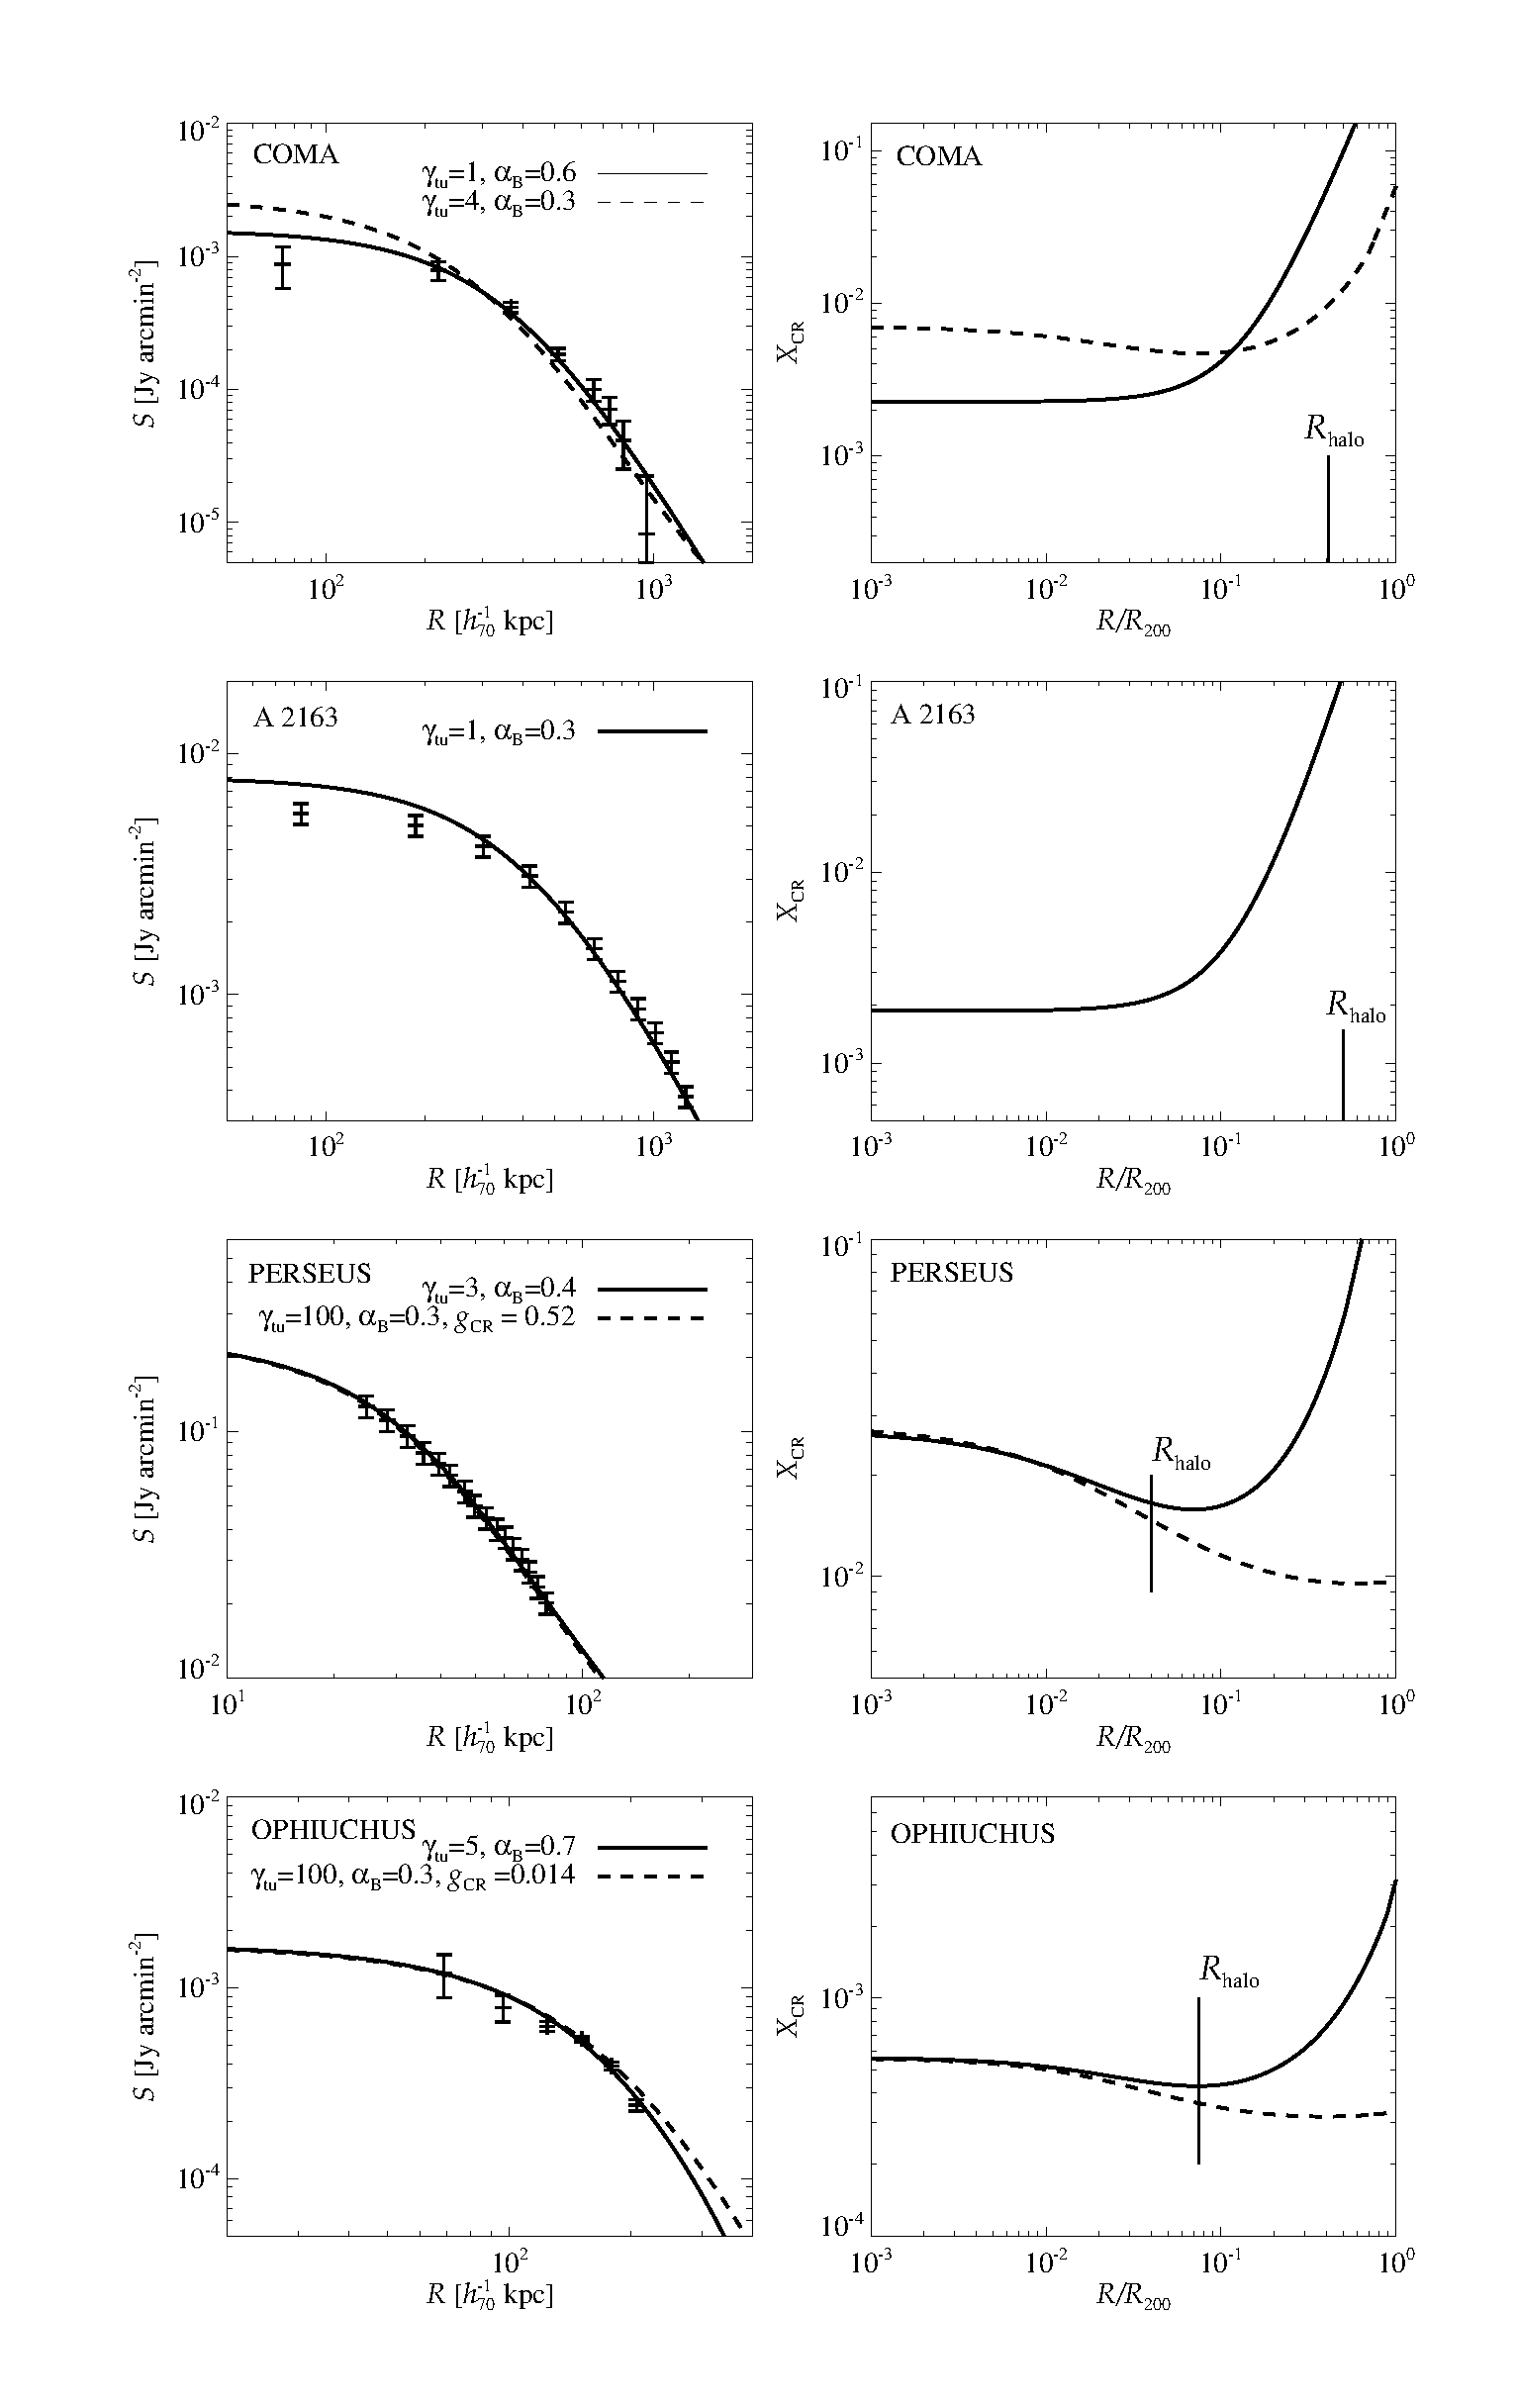
\includegraphics[width=0.75\textwidth]{figures/SB_profiles_ALL.eps}
\caption{Surface brightness modeling of the RHs in Coma, Abell~2163, Perseus and
  Ophiuchus. Left panels show the RHs' azimuthally averaged surface brightness
  profiles, while right panels show the corresponding CR-to-thermal pressure
  profiles $X_{\rmn{CR}}(r)$ where we additionally show the RH radial extension. 
  Note that different parameter values that yield
  almost the same surface brightness profile, result in very different
  $X_{\rmn{CR}}$ profiles. In the case of Abell~2163 and Ophiuchus, we adopt a
  $10\%$ uncertainty range instead of the errors reported by
  \cite{2009A&A...499..679M} to account for additional systematic uncertainties,
  e.g., residual point source contamination. We also adopt a $10\%$ uncertainty
  range for Perseus, for which \cite{1990MNRAS.246..477P} do not report any
  uncertainty intervals.}
\label{fig:SBmodeling}
\end{figure*}


\subsubsection{The Coma radio halo}

The giant radio halo in Coma has a morphology remarkably similar to the extended
X-ray thermal bremsstrahlung emission, although the radio emission declines more
slowly towards the cluster outskirts
\citep{1992A&A...259L..31B,1997A&A...321...55D}. Note that the morphology is
non-spherical, showing an elongation in the East-West direction.  The full-width
half maximum (FWHM) of the radio beam is $0.156$~deg
\citep{1997A&A...321...55D}, almost two orders of magnitude larger than the
X-ray observation of \cite{1992A&A...259L..31B}.\footnote{Note that the apparent
  displacement of the radio and X-ray peak of about $0.05$~deg is well
  within the angular resolution of the radio observation and hence negligible
  for the modeling.}  Thus, we apply a Gaussian smoothing to our theoretical
surface brightness of Equation~(\ref{eq:surf}) with $\sigma_{\rmn{smoothing}} =
FWHM_{\rmn{radio}}/2.355$.

We investigate different values for $\alpha_{\rmn{B}}=(0.3,0.4,0.5,0.6,0.7)$ and
for $\gamma_{\rmn{tu}}$ ranging from 1 to 100. We fix the CR number for
$\gamma_{\rmn{tu}}=100$ using Equation~(36) of \cite{2011A&A...527A..99E}, while
integrating the cluster volume within $R_{200}$, and require CR number
conservation during CR streaming, i.e.~when lowering the values of
$\gamma_{\rmn{tu}}$. Fixing the central magnetic field $B_{0}=5$~$\mu$G
\citep{2010A&A...513A..30B}, we use $g_{\rmn{CR}}$ as normalization factor to
match the radio observations. The best match to the data is obtained for
$\gamma_{\rmn{tu}}=1$ and $\alpha_{\rmn{B}}=0.6$. Values as high as
$\gamma_{\rmn{tu}} \approx 4$ can be accommodated, however, at the expense of a
shallower decline of the magnetic field profile (smaller $\alpha_B$) as a
function of cluster-centric radius. We recover the radio surface brightness
shape and the total radio luminosity within about $20\%$. 

The gamma-ray flux (see Appendix~\ref{app:C}) within $R_{200}$ for the best fit
case and for energies above 100~MeV (100~GeV) is $F_{\gamma} = 4.1 \times
10^{-9}$ ($1.5 \times 10^{-12}$) cm$^{-2}$~s$^{-1}$. Hence, the case of
$\gamma_{\rmn{tu}} = 1$ is in tension with the limit recently set by
\emph{Fermi}-LAT \citep{2012AAS...21920701Z} of $F_{\gamma, UL} (>100~\rmn{MeV})
\approx 2.5 \times 10^{-9}$~cm$^{-2}$~s$^{-1}$.  Note that for slightly higher
values of $\gamma_{\rmn{tu}}$, i.e., a more centrally concentrated CR
distribution, the radio and gamma-ray yield would be increased (assuming CR
number conservation). However, in order to match the observed radio synchrotron
profiles, we have to decrease the CR normalization (parametrized by
$g_{\rmn{CR}}$). This causes the associated gamma-ray flux also to be reduced to
a level that is low enough to easily circumvent the gamma-ray constraints. In
fact, for $\gamma_{\rmn{tu}} = 4$, we obtain $F_{\gamma} (>100~\rmn{MeV}) = 9.6
\times 10^{-10}$~cm$^{-2}$~s$^{-1}$ (and $F_{\gamma} (>100~\rmn{GeV}) = 3.6
\times 10^{-13}$~cm$^{-2}$~s$^{-1}$). We caution that in principle, CR streaming
should cause the CR spectrum to steepen. This may then considerably weaken these
constraints as a result of the convex spectral curvature since the gamma-ray
emission probes the high-energy tail of the CR distribution that is suppressed
in this pictures in comparison to the lower-energy protons that the radio
emission is sensitive to \citep[see][for an extended discussion of this
point]{2011arXiv1111.5544M}.


\subsubsection{The radio halo in Abell~2164}

The morphology of the giant radio halo in Abell~2164 is also closely correlated
to the cluster thermal X-ray structure. As in Coma, the radio emission declines
towards the cluster outskirts at a slower rate in comparison to the thermal
X-ray emission \citep{2001A&A...373..106F}. The morphological appearance is
non-spherical, with an elongation in the East-West direction. We use the surface
brightness map provided by \citet{2009A&A...499..679M} for which the synthesized
radio beam can be approximated by a circular Gaussian with
$FWHM_{\rmn{radio}}=62\arcsec$.  Again, $FWHM_{\rmn{radio}}$ is larger than the
resolution of the ROSAT observation and the corresponding gas density
profile. Converted to physical scale, $\sigma_{\rmn{smoothing}}$ is of the order
of that in Coma because of the larger distance of Abell~2163. Hence, we also apply
Gaussian smoothing.

We follow the same procedure as in Coma, and adopt a central magnetic field
strength of $B_{0}=5~\mu$G. The best fit to the data (and also the only
acceptable fit) is obtained for $\gamma_{\rmn{tu}}=1$ and $\alpha_B=0.3$,
i.e.~the flattest possible surface brightness. We recover the emission shape and
the total luminosity within about $15\%$. The corresponding gamma-ray flux
within $R_{200}$ is $F_{\gamma} (>100~\rmn{MeV}) = 4.2 \times
10^{-10}$~cm$^{-2}$~s$^{-1}$ and $F_{\gamma} (>100~\rmn{GeV}) =1.5 \times
10^{-13}$~cm$^{-2}$~s$^{-1}$, about two orders of magnitude lower than the upper
limit obtained by \emph{Fermi}-LAT \citep{2010ApJ...717L..71A}.


\subsubsection{The Perseus radio mini-halo}

The diffuse radio emission in Perseus is the best known example of a radio-mini
halo \citep{1990MNRAS.246..477P} and Perseus itself is among the best studied
clusters in X-rays
(e.g.,~\citealp{2003ApJ...590..225C,2006MNRAS.366..417F,2011arXiv1105.5025F}). Also
the Perseus radio morphology resembles that in the X-rays. We proceed as before,
but now adopt a higher central magnetic field strength of
$B_{0}=10$~$\mu$G. Such a larger $B_0$ is expected in a CCC with its higher
central gas density, implying a larger adiabatic compression factor of the
magnetic field during the condensation of the cool core (see
\citealp{2010ApJ...710..634A,2011arXiv1111.5544M} for a discussion on the
Perseus magnetic field). The best fit to the data is obtained for
$\gamma_{\rmn{tu}}=3$ and $\alpha_{\rmn{B}}=0.4$, however, values as high as
$\gamma_{\rmn{tu}} \approx 100$, and as low as $\gamma_{\rmn{tu}}=2$, can be
easily accommodated. We recover the surface brightness profile and the total
luminosity within $10\%$.

The gamma-ray flux within $R_{200}$ for the best fit case and for energies above
100~MeV (100~GeV) is $F_{\gamma} = 1.4 \times 10^{-8}$ ($5.1 \times 10^{-12}$)
cm$^{-2}$~s$^{-1}$. Adopting $\gamma_{\rmn{tu}}=100$ and $\alpha_B=0.3$, the
corresponding gamma-ray flux above 100~MeV (100~GeV) is $F_{\gamma} = 4.9 \times
10^{-9}$ ($1.8 \times 10^{-12}$) cm$^{-2}$~s$^{-1}$. Note that the gamma-ray
flux above 100~MeV of the central galaxy NGC~1275 as measured by \emph{Fermi} is
$2 \times 10^{-7}$~cm$^{-2}$~s$^{-1}$ \citep{2009arXiv0904.1904T}, well above
our model predictions due to hadronically produced diffuse gamma-ray emission
that is expected to glow from the entire cluster.

We can compare these predictions with the upper limit above 1~TeV, and for a
region within $0.15$~deg around the cluster center, recently obtained by
\cite{2011arXiv1111.5544M}. For $\gamma_{\rmn{tu}}=3$ ($\gamma_{\rmn{tu}}=100$),
we obtain a flux of $F_{\gamma}(>1~\rmn{TeV},<0.15~\rmn{deg}) = 7.3 \times
10^{-14}$ ($5.5 \times 10^{-14}$) cm$^{-2}$~s$^{-1}$, which is well below the
upper limit of the MAGIC collaboration,
$F_{\gamma,\rmn{UL}}(>1~\rmn{TeV},<0.15~\rmn{deg}) \approx 1.4 \times
10^{-13}$~cm$^{-2}$~s$^{-1}$. Note also that, in the case of $\gamma_{\rmn{tu}}
= 100$, we obtain a maximum CR acceleration efficiency multiplier of
$g(\zeta_{\rmn{p,max}})=0.52$, about half of the value adopted by
\cite{2010MNRAS.409..449P}. Note that we obtain slightly smaller gamma-ray
luminosities in comparison to those predicted by \cite{2010MNRAS.409..449P}
and \cite{2011arXiv1105.3240P} because we additionally account for the
central temperature dip and as well as the decrease towards larger radii.


\subsubsection{The Ophiuchus radio mini-halo}

The Ophiuchus cluster has been widely studied both in radio and X-rays in the
last few years because of the claimed presence of a non-thermal hard X-ray tail
\citep{2008A&A...479...27E,2008PASJ...60.1133F,2009A&A...499..371G,
  2009A&A...499..679M,2009MNRAS.396.2237P,2009A&A...508.1161N,2010A&A...514A..76M,
  2010MNRAS.405.1624M}.  It was classified as a merging cluster by
\cite{2001PASJ...53..605W}, but more recently \cite{2008PASJ...60.1133F} did not
find any evidence of merging and, on the contrary, classified it as one of the
hottest clusters with a cool-core (see also \citealp{2010MNRAS.405.1624M}). The
radio mini-halo morphology displays similarities with the thermal X-ray
emission. For our modeling we use the surface brightness profile provided by
\cite{2009A&A...499..679M}.  

We proceed as before, adopting a central magnetic field value of
$B_{0}=10$~$\mu$G. The best fit to the data is obtained for
$\gamma_{\rmn{tu}}=5$ and $\alpha_B=0.7$. However, values as high as
$\gamma_{\rmn{tu}} \approx 100$, and as low as $\gamma_{\rmn{tu}}=2$, can be
easily accommodated. We recover the surface brightness profile and the total
luminosity within $20\%$. The gamma-ray flux within $R_{200}$ for the best
fit case and for energies above 100~MeV (100~GeV) is $F_{\gamma} = 1.2 \times
10^{-10}$ ($4.3 \times 10^{-14}$) cm$^{-2}$~s$^{-1}$. Adopting
$\gamma_{\rmn{tu}}=100$ and $\alpha_B=0.3$, the corresponding gamma-ray flux
above 100~MeV (100~GeV) is $F_{\gamma} = 8.3 \times 10^{-11}$ ($3.1 \times
10^{-14}$) cm$^{-2}$~s$^{-1}$. The gamma-ray flux is, in both cases, about two
orders of magnitude lower than the upper limit obtained by \emph{Fermi}-LAT
\citep{2010ApJ...717L..71A}. Note also that in the case of $\gamma_{\rmn{tu}} =
100$ we obtain a maximum CR acceleration efficiency multiplier of
$g(\zeta_{\rmn{p,max}})=0.014$.

%The position of radio and X-ray peaks seems displaced by about 24''. Again,
%Matteo Murgia has kindly provided the radio surface brightness computed with
%respect to the \cite{2002ApJ...567..716R} X-ray position, however the change is
%not very significant.

\subsection{Discussion and conclusions on the hybrid hadronic model}

After these detailed considerations on four individual RHs, we
are now summarizing the main points:
\begin{enumerate} 
\item The radio mini-halos in Perseus and Ophiuchus can be easily reproduced in
  our hybrid hadronic model with a wide range of possible values for
  $\gamma_{\rmn{tu}}$. In contrast, the large extension of the giant radio halos
  in Coma and Abell~2164 in comparison to the X-ray emission requires lower
  values of $\gamma_{\rmn{tu}}\lesssim3$ in order to get acceptable model
  fits. However, we would expect higher values for $\gamma_{\rmn{tu}}$ in
  merging NCCCs \citep{2011A&A...527A..99E}.  There are three main factors that
  render the merging NCCC fits not conclusive and may alleviate this problem.
  (i) Primary electrons accelerated in outer shocks, which we do not consider,
  could have an important contribution to the RH emission, particularly in the
  cluster outskirts \citep{2008MNRAS.385.1211P}.  (ii) Merging clusters are not
  spherically symmetric as can be seen in Coma and Abell~2164, requiring
  non-spherical modelling in the future. (iii) Adopting the simulation-derived
  $\tilde{C}$ profile \citep{2010MNRAS.409..449P} for our hybrid model may have
  biased the inner slope of the CR density profile to become too steep due to
  the overcooling problem of purely radiative simulations resulting in values of
  $\gamma_{\rmn{tu}}$ that are biased low in comparison to a potentially
  shallower slope of the inner CR profile. To quantify the last point, we fit
  the Coma surface brightness using a model without $\tilde{C}$. We find that
  values as high as $\gamma_{\rmn{tu}} \approx 8$ can be accommodated. However,
  $\gamma_{\rmn{tu}}=1$ still represents the best fit model, demonstrating that
  the problem can be weakened but not circumvented even in this case of a cored
  CR profile. Nevertheless, we can successfully reproduce the morphology of Coma
  and Abell~2163 RHs fairly well, solving the previous problems of the
  \emph{classical} hadronic model (see e.g.~\citealp{2010MNRAS.401...47D}).
\item Gamma-ray and radio emission are complementary tools in constraining the
  CR population. While gamma-ray emission is a direct way to constrain the CR
  pressure, it is also critical in disentangling between the hadronic and
  re-acceleration model. In contrast, the information derived from the radio
  window is degenerate with the assumptions on the magnetic field
  strengths. Nevertheless, we find that RH measurements allow tighter constraints
  on the CR pressure (except for the case of Coma).  However, gamma-ray
  predictions should be lowered with respect to previous results
  \citep{2010MNRAS.409..449P,2011arXiv1105.3240P} in light of the results
  presented here (see also \citealp{2011A&A...527A..99E}).
\item The magnetic field values adopted here are perfectly in agreement with
  other observational constraints, solving previous tensions of the
  \emph{classical} hadronic model (see
  e.g.~\citealp{2011ApJ...728...53J}). Indeed, different values of $B_{0}$ could
  be adopted without violating other observational constraints. The exception to
  this is again Coma, for which a higher $B_{0}$ value would be in contradiction
  with Faraday rotation measure data \citep{2010A&A...513A..30B}, while a value
  much lower would imply a level of the gamma-ray emission that challenges the
  most recent {\em Fermi} limit \citep{2012AAS...21920701Z}.
\item Considering the case of advection-dominated CR transport
  ($\gamma_{\rmn{tu}}\gtrsim100$), which only allows a good description of the
  data for Perseus and Ophiuchus, the $g_{\rmn{CR}}$ parameter can be
  interpreted as the maximum CR acceleration efficiency used in
  \cite{2010MNRAS.409..449P}. If the cluster CR population is mainly accelerated
  in cosmological structure formation shocks, then this value should depend on
  the mass accretion history and to be approximately universal, i.e.~similar for
  all clusters. We find $g_{\rmn{CR, Perseus}} = 0.52$ and $g_{\rmn{CR,
      Ophiuchus}} = 0.014$, because we fixed $B_{0}=10$~$\mu$G in both cases and
  used $g_{\rmn{CR}}$ as normalization. This discrepancy can be resolved by
  increasing/lowering the central magnetic field in Perseus/Ophiuchus to
  $B_{0,\rmn{Perseus}}=20$~$\mu$G and $B_{0,\rmn{Ophiuchus}}=1$~$\mu$G. We note,
  however, that without the guidance of cosmological cluster simulations that
  include CR streaming, the data does not yet constrain $\gamma_{\rmn{tu}}$.
\item The small cluster sample analysed here was only meant to serve as a proof
  of concept and to demonstrate the viability of matching observed RH data with
  our hybrid hadronic model. This is in especially true because of the
  comparably large parameter space that the physics modeled here demands and
  which encompasses our parametrization of the magnetic field ($B_0$,
  $\alpha_B$), $\gamma_{\rmn{tu}}$ and the CR acceleration efficiency
  function. Particularly, a large region of the ($\gamma_{\rmn{tu}}$,
  $\alpha_{\rmn{B}}$) parameter space is available for the analyzed radio
  mini-halos (note also that the parameters $\gamma_{\rmn{tu}}$ and
  $\alpha_{\rmn{B}}$ are degenerate). Future work on all known RHs may provide
  better insight, but is beyond the scope of this work.
\end{enumerate}
Summarizing, the hybrid hadronic model successfully reproduces the main
morphological characteristics of both giant and mini-halos without violating
gamma-ray constraints. As we will see in the next section, it can also reproduce
the radio-to-X-ray scaling relation, solving the previous problems of the
\emph{classical} hadronic model, and the radio-to-SZ scaling relation. 


%%%%%%%%%%%%%%%%%%%%%%%%%%%%%%%%%%%%%%%%%%%%%%%%%%%%%%%%%%%%%%%%%%%
%%%%%%%%%%%%%%%%%%%%%%%%%%%%%%%%%%%%%%%%%%%%%%%%%%%%%%%%%%%%%%%%%%%
\begin{figure*}[t]
\centering
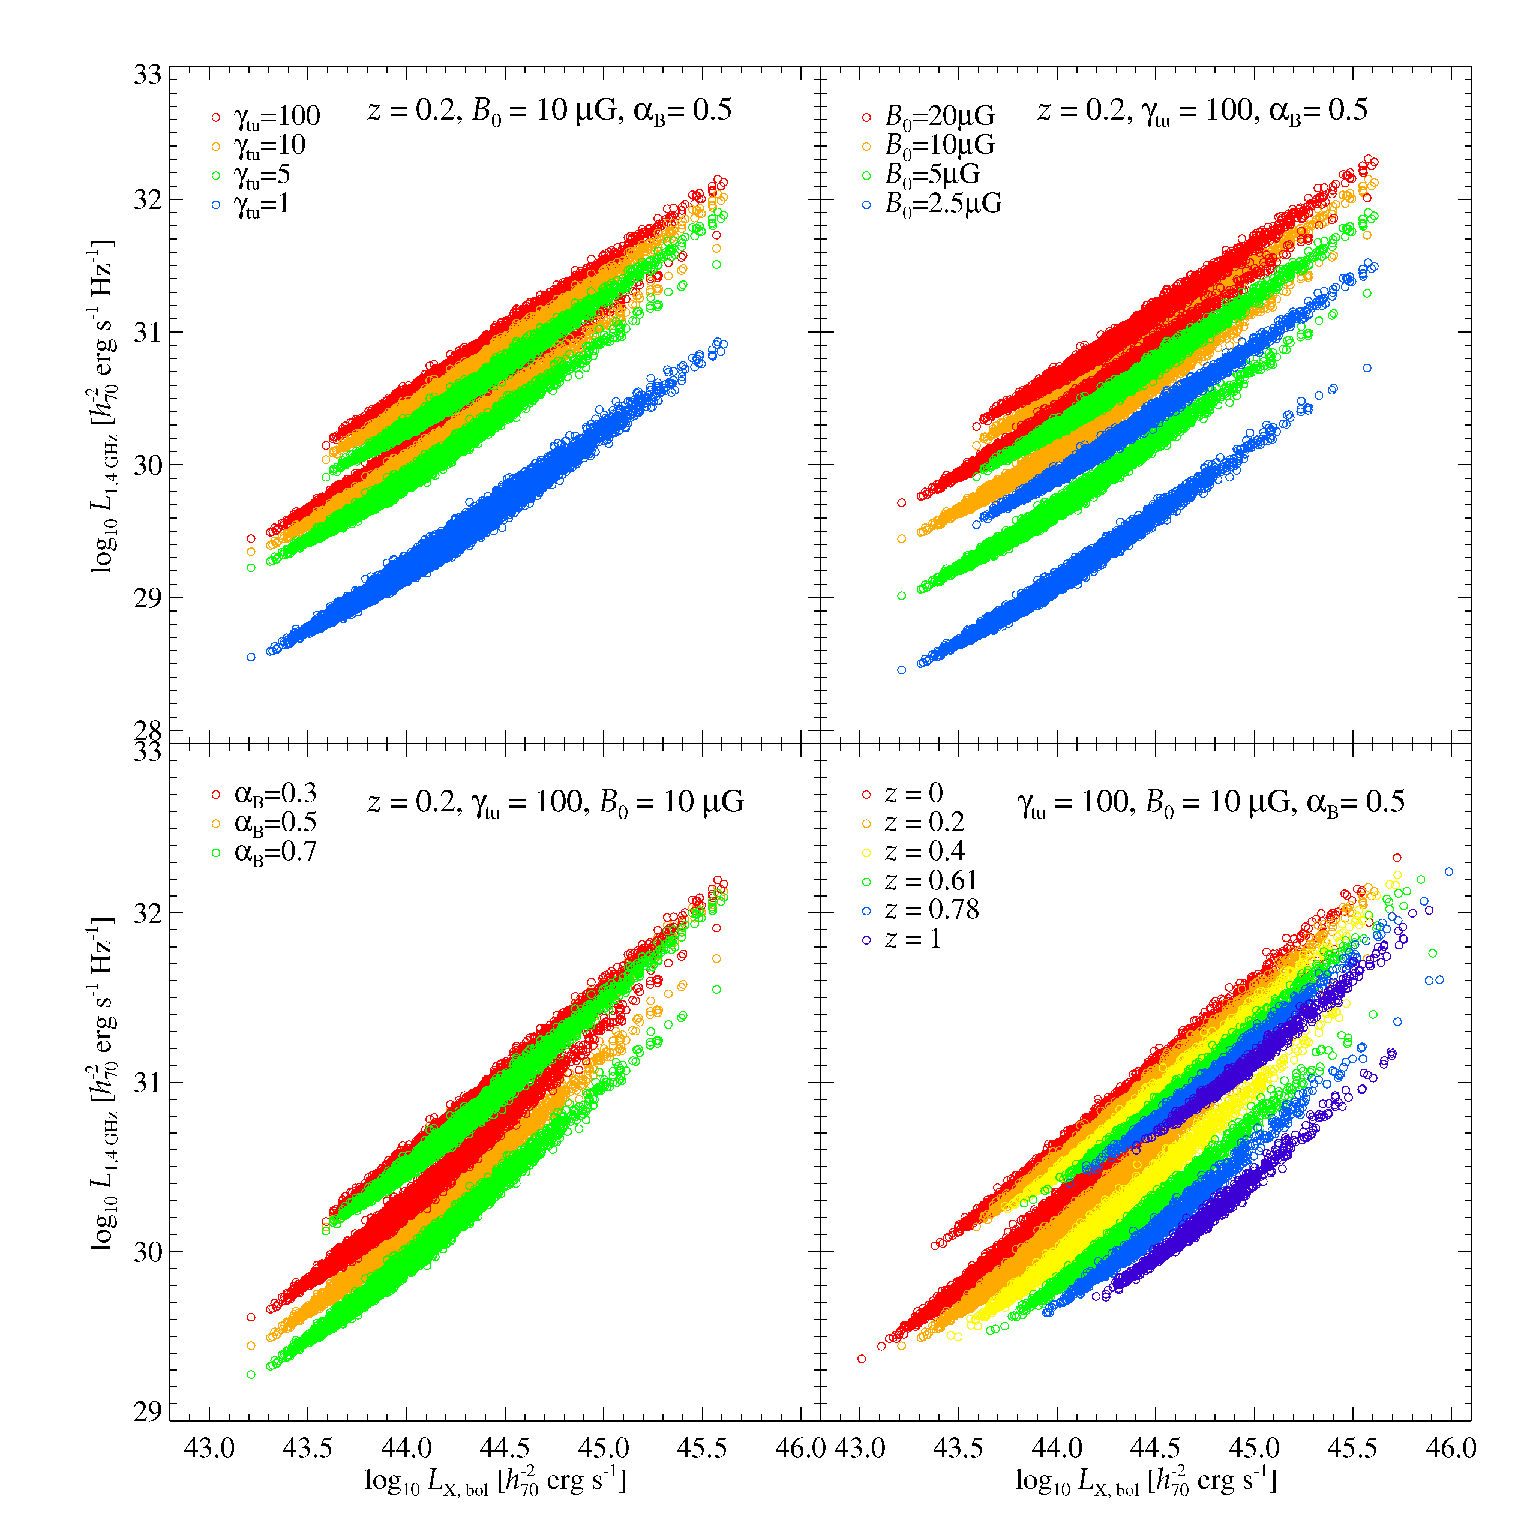
\includegraphics[width=0.49\textwidth]{figures/PL_relation_testing_gimp.eps}
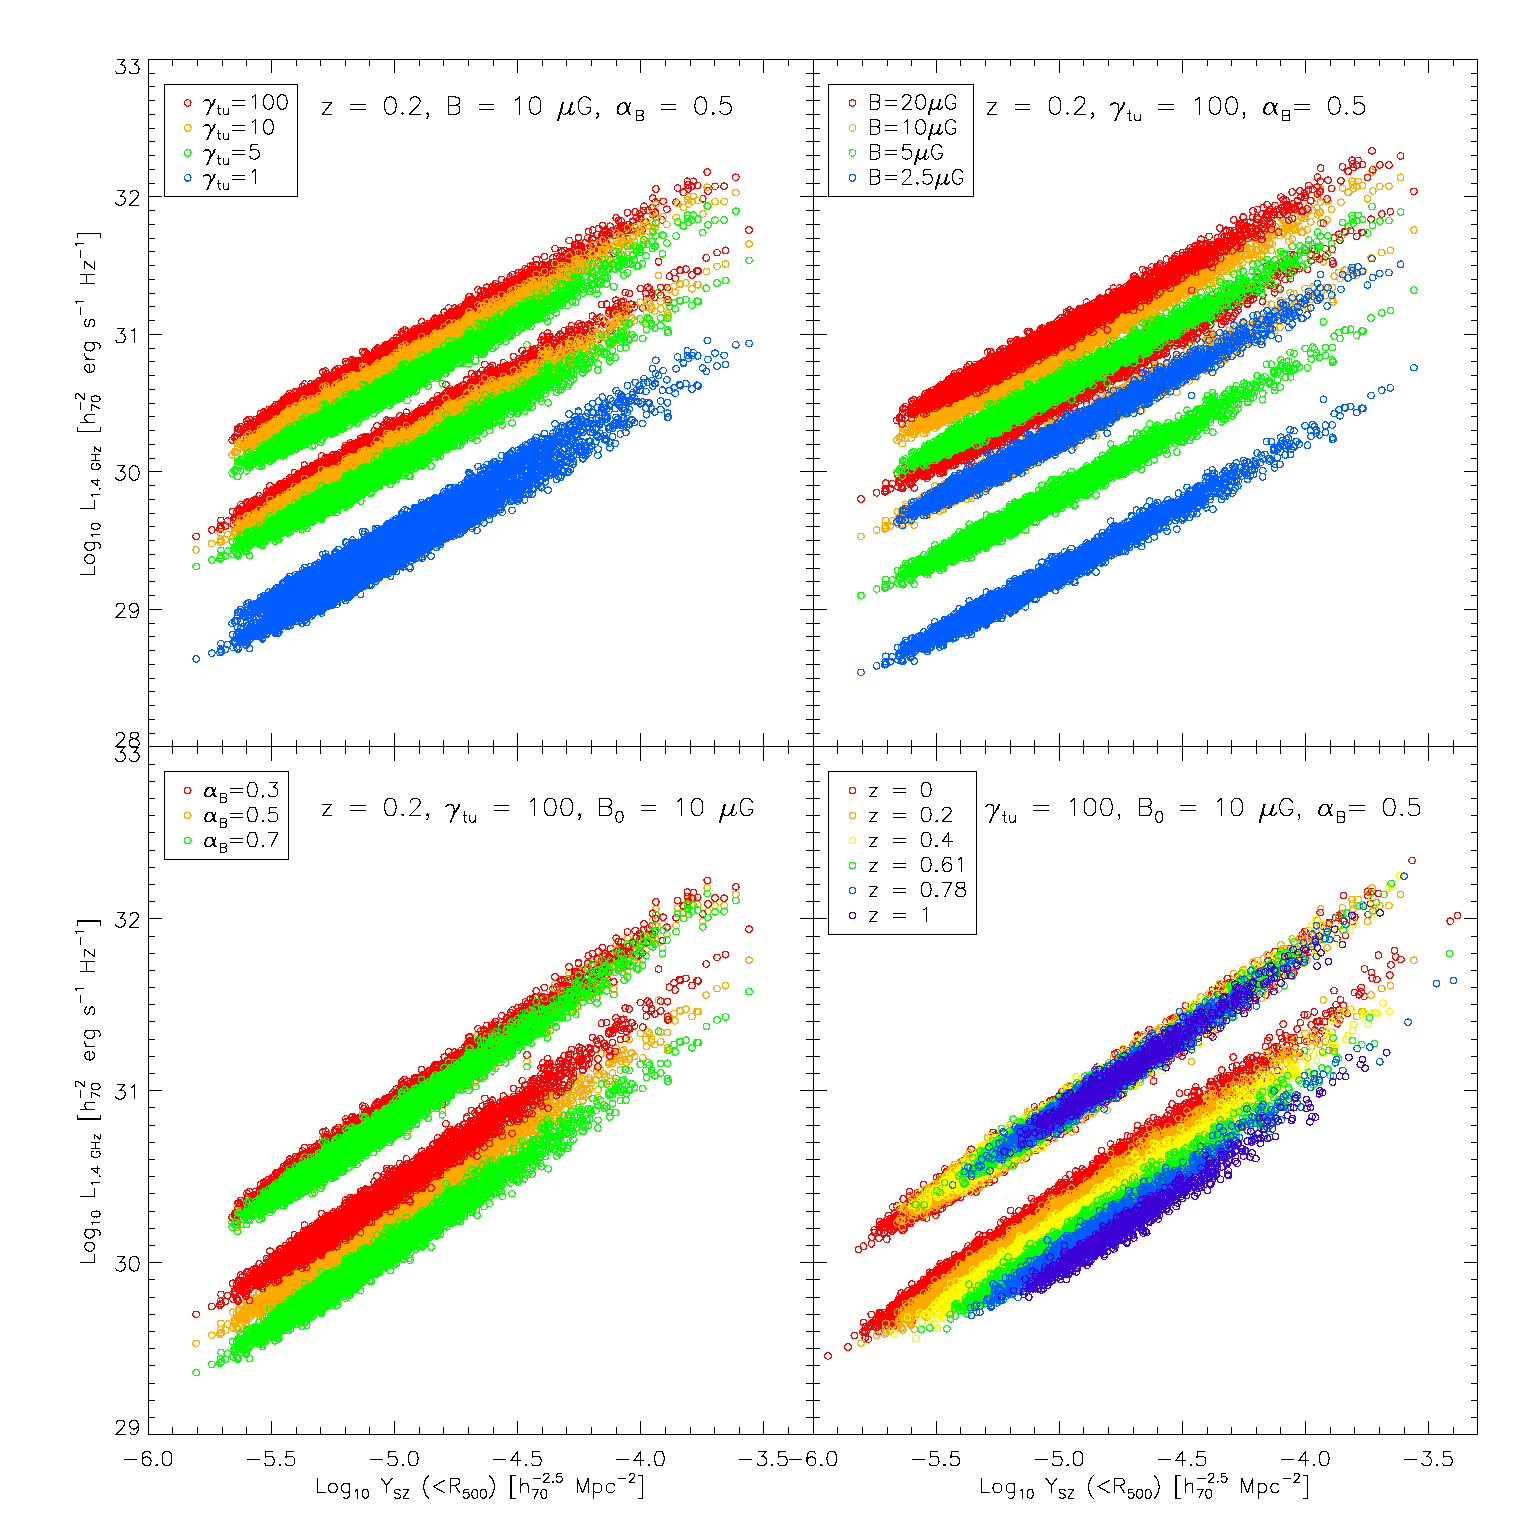
\includegraphics[width=0.49\textwidth]{figures/PSZ_relation_testing_gimp.eps}
\caption{Radio-to-X-ray and radio-to-SZ scaling relations as predicted by our
  final CR model. In the left panel, we show how the
  $L_{1.4~\rmn{GHz}}-L_{\rmn{X,bol}}$ relation varies upon changing different
  parameters. In the right panel, we show the same, but for the
  $L_{1.4~\rmn{GHz}}-Y_{\rmn{SZ},500}$ relation. Note that in each plot there
  are two separated populations for each model realization. The upper sets of
  points correspond to the CCC population while the lower sets correspond to
  NCCCs. The plot labels indicate those parameters which are kept
  fixed. We fix the $g_{\rmn{CR}}$-normalization parameter to 0.5 for all
  cases. See main text for details. {\bf change colors?}}
\label{fig:SR}
\end{figure*}


\section{Radio Scaling Relations}
\label{sec:4}
As introduced in Section~\ref{sec:1}, there exist an apparent bimodality between
the radio and X-ray cluster emission. Clusters with a given X-ray luminosity can
either host RHs or show an absence of diffuse radio emission
(e.g.~\citealp{2009A&A...507..661B,2011A&A...527A..99E}). More recently, a study
of the radio-to-SZ scaling relation revealed the absence of a strong bimodality
dividing the cluster population into radio-loud and radio-quiet clusters
\citep{2012MNRAS.421L.112B}. Since $Y_{\rmn{SZ}}$ correlates more tightly with
cluster mass than $L_{1.4~\rmn{GHz}}$, this may indicate that the larger scatter
of $L_{1.4~\rmn{GHz}}$ correlates with the radio luminosity in such a way that
it produces a bimodality; but as a result of a second (hidden parameter) rather
than the fundamental cluster parameter -- its mass. In this section, we
investigate these two scaling relations in the framework of our extended
hadronic scenario.


\subsection{Exploring the parameter space of scaling relations}

In Figure~\ref{fig:SR}, we show the general scaling relations of our final CR
model of Section~\ref{sec:2.3} applied to the MultiDark sample. We show how both
the radio-to-X-ray and the radio-to-SZ scaling relations differ upon varying the
parameters $\gamma_{\rmn{tu}}$, $B_{0}$, $\alpha_{\rmn{B}}$ and redshift. We fix
the CR-normalization parameter $g_{\rmn{CR}}$ to 0.5 in all cases, ensuring an
average CR-to-thermal pressure of $2\%$ ($0.05\%$) within $R_{500}$
($R_{500}/2$). Here, the radio luminosity is calculated at $1.4$~GHz within
$R_{500}.$\footnote{The mean (median) difference between calculating $L_{\nu}$
  within $R_{200}$ or $R_{500}$ is 5.3\% (5.6\%).}  In our CR model, we fix the
CR number for $\gamma_{\rmn{tu}}=100$ using Equation~(36) of
\cite{2011A&A...527A..99E}, integrating up $R_{500}$. To compute the radio
luminosity for different values of $\gamma_{\rmn{tu}}$, we employ CR number
conservation (for energies $E>$~GeV where Coulomb cooling is negligible for CR
protons).

In each panel in Figure~\ref{fig:SR} there are two separated populations for
each model realization (i.e., for a given set of parameters). Each upper set of
points corresponds to the CCC population while the lower set corresponds to
NCCCs, respectively. In our model, the radio and X-ray emissivities scale with
the square of the gas density so that $L_{1.4~\rmn{GHz}}$ and $L_{\rmn{X,bol}}$
are significantly higher for CCCs in comparison to NCCCs. In contrast,
$Y_{\rmn{SZ}}$ only depends weakly on the central gas density as explained in
Sec.~\ref{sec:X-SZ-scaling}. This explains the relative location of the NCCC and
CCC populations in the $L_{1.4~\rmn{GHz}}-L_{\rmn{X,bol}}$ and
$L_{1.4~\rmn{GHz}}-Y_{\rmn{SZ}}$ planes. In reality, we expect an (ab initio
unknown) distribution of these parameters which would substantially increase the
scatter in the scaling relations and possibly lead to a bimodality, depending on
correlations among the different parameters.


\subsection{Comparison to observations}
\label{sec:scaling-obs}

\begin{figure*}[t]
\centering
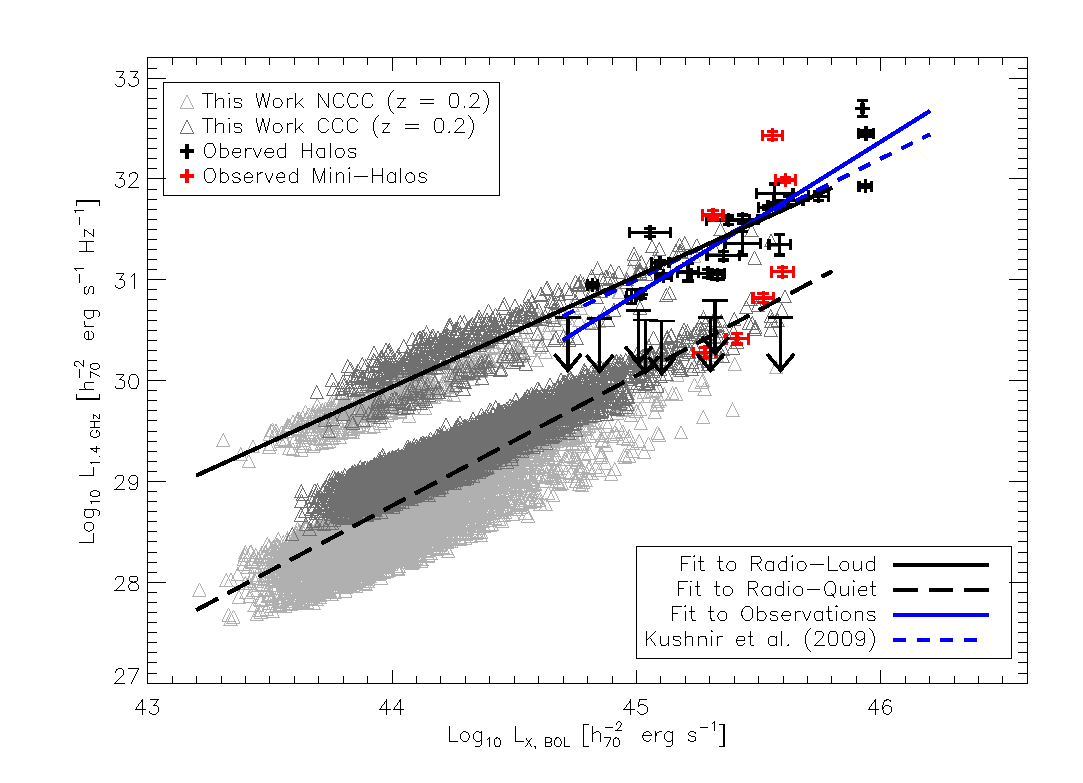
\includegraphics[width=0.49\textwidth]{figures/PL_relation.eps}
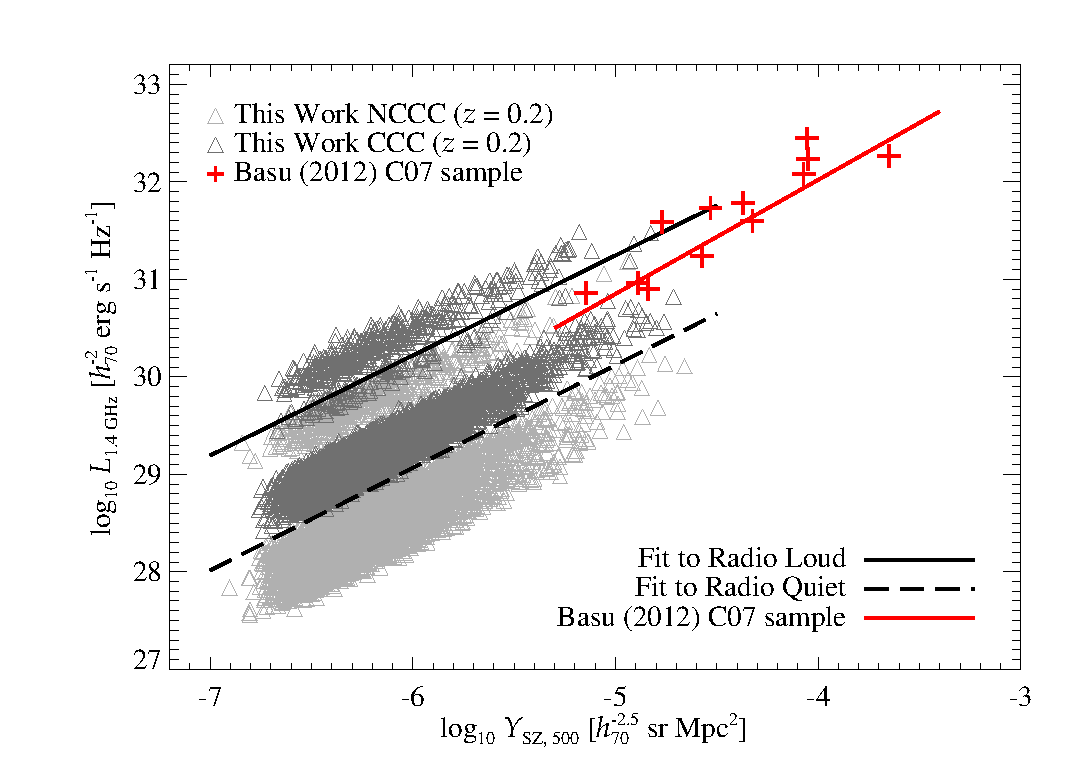
\includegraphics[width=0.49\textwidth]{figures/PSZ_relation.eps}
\caption{Radio-to-X-ray and radio-to-SZ scaling relations in our final CR model
  (see main text for the details of the chosen parameters) compared with
  observations.  \emph{Left.} $L_{1.4~\rmn{GHz}}-L_{\rmn{X,bol}}$ relation in
  comparison to the observational sample taken from the literature and detailed
  in Appendix~\ref{app:D}. \emph{Right.} $L_{1.4~\rmn{GHz}}-Y_{\rmn{SZ}}$
  relation in comparison to the observational sample C07 from
  \cite{2012MNRAS.421L.112B}.}
\label{fig:PLSZ}
\end{figure*} 
 
After collecting the X-ray luminosity and the SZ flux of known RHs, we compare
the resulting scaling relations to a phenomenological model realization that was
chosen to additionally obey other observational constraints (e.g., from Faraday
rotation studies) as well as theoretical considerations of CR transport.


\subsubsection{Observational sample}

In Appendix~\ref{app:D} we construct a (literature-)complete sample of giant
radio halos (black) and radio mini-halos (red), as well as upper limits on the
radio emission \citep{2009A&A...507..661B, 2011A&A...527A..99E,
  2009A&A...499..371G}, and show this in the left panel of
Figure~\ref{fig:PLSZ}. The median redshift of this sample is $z\approx0.18$. The
corresponding observational scaling relation is well fit by $\log_{10}
L_{1.4~\rmn{GHz}} = A + B~\log_{10} L_{\rmn{X,bol}}$ with $A=-50.433\pm2.226$
and $B=1.803\pm0.049$, and a scatter of $\sigma_{yx} \approx 0.44$ (we do not
include upper limits in the fit; units are as in Figure~\ref{fig:PLSZ}). We
refer the reader to \cite{2009A&A...507..661B} and \cite{2011A&A...527A..99E}
for an extensive discussion on this topic. We emphasize that in contrast to
giant radio halos, mini-halos span a wider range in radio luminosity (as also
pointed out by \cite{2009A&A...499..679M}). The Perseus mini-halo (highest radio
mini-halo luminosity in the left panel of Figure~\ref{fig:PLSZ}), e.g., has a
radio luminosity that is almost an order of magnitude higher than in giant radio
halos at the same X-ray luminosity. In contrast, the Ophiuchus mini-halo (lowest
radio mini-halo luminosity in the left panel of Figure~\ref{fig:PLSZ}), which is
representative of a few other similar examples recently detected in CCCs
(i.e.~A2029 and A1835), has a radio luminosity which is much lower than giant
radio halos in merging clusters and even below the upper limits. 

We caution that the determination of the slope of the $L_{1.4}-L_{\rmn{X,bol}}$
relation is not very robust because of the small sample size of RHs, selection
biases of extended low-surface brightness objects, and systematic uncertainties
in the measurements of $L_{1.4}$ and $L_{\rmn{X,bol}}$. The recently detected
low-luminosity mini-halos exemplify those uncertainties and the large intrinsic
scatter of this relation. On the other hand, X-ray luminosities for the same
object as derived by, e.g.,~ROSAT and \emph{Chandra} can easily differ by a
factor of a few. In the left panel of Figure~\ref{fig:PLSZ}, we additionally
show the model of \citet{2009JCAP...09..024K} with a sloped of $\approx1.2$,
arbitrarily normalized for visual purposes, from their simple analytical
hadronic model.

For the comparison to the observed 1.4~GHz radio-to-SZ scaling relation, we use
the result by \cite{2012MNRAS.421L.112B} that is based on the radio halo sample
from \cite{2007MNRAS.378.1565C} (hereafter C07; median redshift of $z \approx
0.18$; note that no mini-halos are included). For this sample,
\cite{2012MNRAS.421L.112B} computes $Y_{\rmn{SZ}}$ within the radio-halo radii
given by \cite{2007MNRAS.378.1565C}. These radii have a median of about
$0.5$~$h_{70}^{-1}$~Mpc which compares favourably with the median of $R_{500}
\approx 0.4$~$h_{70}^{-1}$~Mpc in our MultiDark $z = 0.2$ snapshot. For the C07
sample, \cite{2012MNRAS.421L.112B} obtains a scaling relation in the form of
$\log_{10} L_{1.4~\rmn{GHz}} = A + B~\log_{10} Y_{\rmn{SZ}}$ with $A=29.7\pm0.8$
and $B=1.17\pm0.18$, and a scatter of $\sigma_{yx} \approx 0.28$ (units are as
in Figure~\ref{fig:PLSZ}). The same comments regarding the small sample size of
RHs, selection biases, and systematic uncertainties in the luminosity
measurements also apply here. Future studies are needed to improve the
observational situation.


\subsubsection{Model realization}

In order to compare our model prediction with observations, we select a
particular realization of our model. To this end, we use the MultiDark cluster
sample at $z=0.2$, which compares well with the redshift of the observational
samples; see below and Appendix~\ref{app:D}. We divide our cluster sample
randomly into radio-quiet and radio-loud clusters, assuming a ratio of $10\%$ of
the latter. We use the turbulent propagation parameter $\gamma_{\rmn{tu}}$ to
separate both populations. In radio-quiet clusters, we assign
$\gamma_{\rmn{tu}}=1$ and in radio-loud clusters, we adopt randomly and
uniformly $\gamma_{\rmn{tu}}$ values in the intervals $[40,80]$ and $[1,5]$ for
NCCCs and CCCs, respectively.

Our modeling of magnetic fields is inspired by Faraday rotation studies that
point to higher field values in the core region of CCCs compared to NCCCs
\citep{2011A&A...529A..13K, 2010A&A...513A..30B}, presumably due to the higher
adiabatic compression factor during the formation of the cooling core. Hence,
for radio-quiet clusters, we adopt randomly and uniformly distributed values of
the central magnetic field $B_0$ in the intervals $[2.5,5.5]$~$\mu$G and
$[5,10]$~$\mu$G for NCCCs and CCCs, respectively. To account for the potential
turbulent dynamo in radio-loud objects (characterized by a higher turbulent
transport parameter in our model), we slightly increase $B_0$ in those objects
and chose $B_0$ intervals of $[4.5,7.5]$~$\mu$G and $[7.5,12.5]$~$\mu$G for
NCCCs and CCCs, respectively.

We fix $\alpha_{\rmn{B}}=0.5$ and $g_{\rmn{CR}}=0.5$ for all clusters; the
latter choice ensures a median average CR-to-thermal pressure of about $2\%$
($0.05\%$) within $R_{500}$ ($R_{500}/2$). We note that these choices are
phenomenologically driven with the aim to reproduce observations. The parameter
study in Fig.~\ref{fig:SR} exemplifies considerable degeneracies so that
different combinations of parameters can potentially result in very similar
distributions of $L_{1.4~\rmn{GHz}}$ and $L_{\rmn{X,bol}}$. We emphasize the
need of more detailed observations of radio halos and in particular of
multi-frequency correlation studies to constrain the interplay of some of these
parameters. 

In Figure~\ref{fig:PLSZ}, we show our model in comparison to the observed
radio-to-X-ray and radio-to-SZ scaling relations. The normalization of our model
can be arbitrarily varied by changing $g_{\rmn{CR}}$ as long as the resulting
$X_{\rmn{CR}}$ respects the current observational constraints
(e.g.~\citealp{2011arXiv1111.5544M}) and remains below few percents. As
explained above, our choice of $g_{CR}=0.5$ ensures an average CR-to-thermal
pressure of $2\%$ within $R_{500}$, allowing thus plenty of available parameter
space to match the observational constraints.  Our model is sufficiently
flexible to either mimic a cluster radio bimodality or not, depending on the
parameters adopted for the populations of radio-loud and radio-quiet
objects. 

However, with a given model realization as in Figure~\ref{fig:PLSZ}, the
separation of the radio-loud and quiet populations is substantially larger in
the $L_{1.4~\rmn{GHz}}-L_{\rmn{X,bol}}$ plane than in the
$L_{1.4~\rmn{GHz}}-Y_{\rmn{SZ}}$ plane, which exhibits almost a continuum
distribution from radio-loud CCCs to the radio-quiet NCCCs. This is mainly
because the bolometric X-ray emissivity scales with $\rho_{\rmn{gas}}^2$ while
$Y_{\rmn{SZ}}\propto\rho_{\rmn{gas}}$ (which is only strictly valid for an
isothermal gas distribution). As a consequence, the highly peaked gas profiles
of CCCs have less impact on $Y_{\rmn{SZ}}$ than on $L_{\rmn{X,bol}}$. This is
one plausible explanation for the observed discrepancy of the presence of a
bimodality in $L_{1.4~\rmn{GHz}}-L_{\rmn{X,bol}}$ and the apparent absence of it
in $L_{1.4~\rmn{GHz}}-Y_{\rmn{SZ}}$. 

The slope of our model depends on the different parameter choices and,
particularly, on the relative differences introduced for the NCCC/CCC and the
radio-loud/quiet populations. However, we note that our
$L_{1.4~\rmn{GHz}}-L_{\rmn{X,bol}}$ is slightly shallower than the observed
relation, more similar to the \cite{2009JCAP...09..024K} prediction, and that
the slope of our $L_{1.4~\rmn{GHz}}-Y_{\rmn{SZ}}$ compares well with the
observed slope. Owing to the many uncertainties and lack of robustness both in
the observations and modeling at this stage, we do not attempt to fine-tune our
model to observations.


%%%%%%%%%%%%%%%%%%%%%%%%%%%%%%%%%%%%%%%%%%%%%%%%%%%%%%%%%%%%%%%%%%%
%%%%%%%%%%%%%%%%%%%%%%%%%%%%%%%%%%%%%%%%%%%%%%%%%%%%%%%%%%%%%%%%%%%
\section{Radio Luminosity Function}
\label{sec:5}

\begin{figure*}[t]
\centering
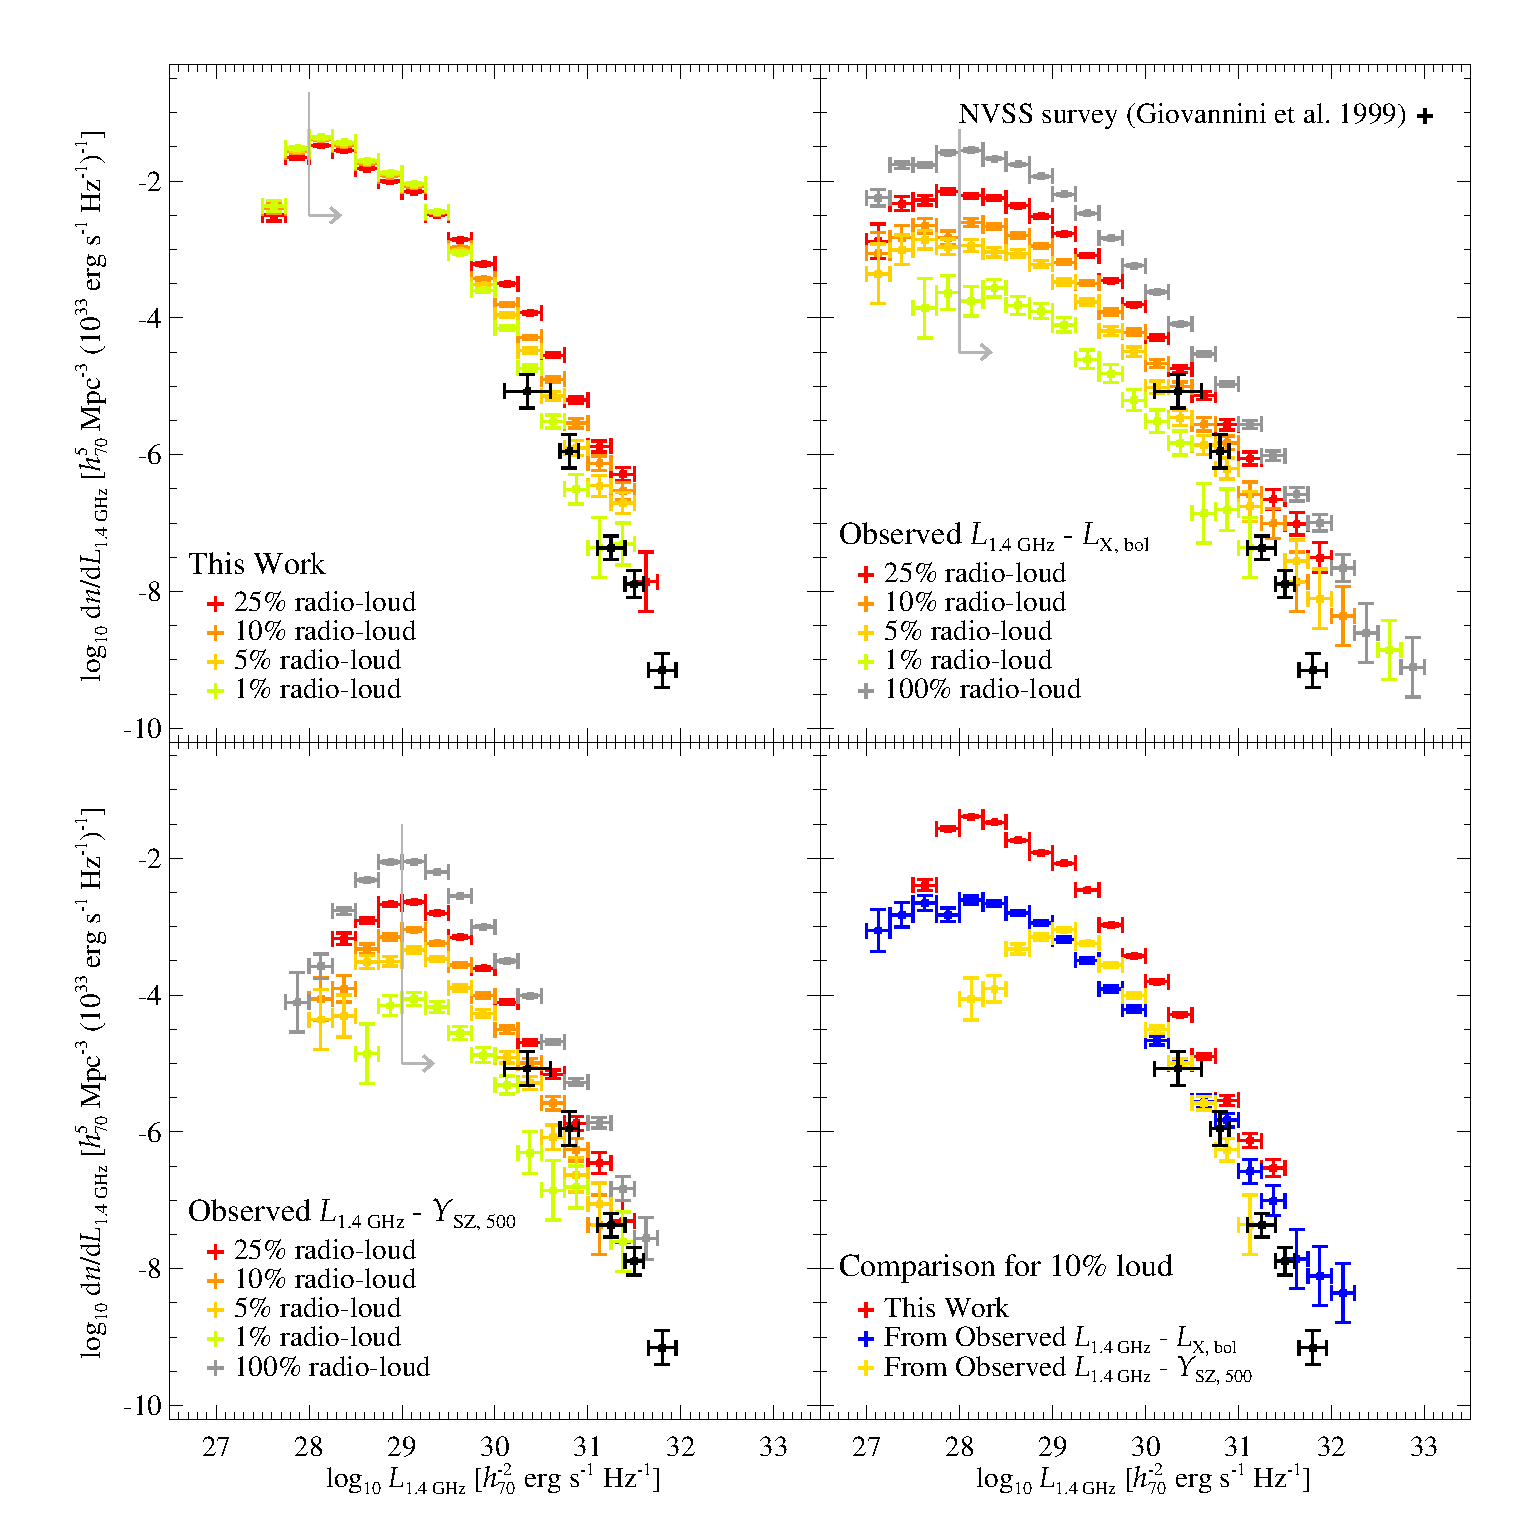
\includegraphics[width=0.85\textwidth]{figures/RLFs_1.4.eps}
\caption{Radio luminosity function (RLF) at 1.4~GHz. The top left panel shows
  the RLF of our final CR model (see main text for the details of the chosen
  parameters) for different fractions of radio-loud clusters. Additionally shown
  is the contribution of radio-quiet and loud populations to the total RLF
  (assuming a fraction of $25\%$ and $1\%$ of radio-load objects). The top right
  panel shows the RLF obtained by applying the observed
  $L_{1.4~\rmn{GHz}}-L_{\rmn{X,bol}}$ relation to the MultiDark clusters at $z =
  0.2$, using our phenomenological gas model for $L_{\rmn{X,bol}}$ of each
  cluster; again for different percentages of radio-loud clusters.  The bottom
  left panel shows the RLF obtained by applying the observed
  $L_{1.4~\rmn{GHz}}-Y_{\rmn{SZ}, 500}$ relation to the MultiDark clusters at $z
  = 0.2$, using the $Y_{\rmn{SZ}, 500}$ of our our phenomenological gas model
  for each cluster. The bottom right panel shows the comparison between the
  three approaches for 10\% of radio-loud clusters. The NVSS survey RLF
  \citep{1999NewA....4..141G} is shown for comparison in all panels. Horizontal
  error bars represent the mass bins while the vertical error bars are
  Poissonian uncertainties. Apart from correcting for incomplete sky coverage,
  no other incompleteness corrections have been applied.  The light gray line
  marked by the arrow estimates the incompleteness limit owing to the adopted
  low-mass cut (see Section~\ref{sec:2}) and the scatter in the halo
  luminosities.}
\label{fig:RLF_1.4}
\end{figure*}


\subsection{Comparison with observations at 1.4~GHz}

In Figure~\ref{fig:RLF_1.4}, we show the RH luminosity function (RLF) at 1.4~GHz
for a representative realization of our final CR model (as in
Sect.~\ref{sec:4}), and compare it with observational results. As for the X-ray
emission, the RLF is completely determined by the cluster mass function and the
radio luminosity-to-mass relation, through $L_{1.4~\rmn{GHz}}-L_{ \rmn{X,bol}}$
or $L_{1.4~\rmn{GHz}}-Y_{\rmn{SZ}}$ in combination with our phenomenological gas
model with the additional uncertainty of the fraction of radio-loud
clusters. Thus, in Figure~\ref{fig:RLF_1.4}, we also show the ``true'' RLFs
obtained by applying the $L_{1.4~\rmn{GHz}}-L_{\rmn{X,bol}}$ and
$L_{1.4~\rmn{GHz}}-Y_{\rmn{SZ}}$ relations to simulated clusters of the
MultiDark snapshot at $z = 0.2$, using our phenomenological gas model for
$L_{\rmn{X,bol}}$ and $Y_{\rmn{SZ}, 500}$ of each cluster, respectively. Note
that this procedure is {\em only} applied to halos defined as radio-loud
clusters (which are by definition accounted for in the $L_{1.4~\rmn{GHz}}$
scaling relations) and we assume a fraction of 100\%, 25\%, 10\%, 5\% and 1\% of
radio-loud clusters. As evident from Figure~\ref{fig:RLF_1.4}, this is different
from our model for the radio luminosity, where we also define a fraction of
radio-loud cluster. However, the radio-quiet population also contributes to the
RLF with an increasing fraction at low luminosities. This is exemplified in the
top left plot of Figure~\ref{fig:RLF_1.4}, which shows the contribution of
radio-quiet and loud populations to the total RLF, assuming a fraction of $25\%$
and $1\%$ of radio-load objects.

In Appendix~\ref{app:D}, we make an attempt to construct a RLF from existing
X-ray flux-limited radio surveys. There exist two such studies, the cluster
radio survey done with the National Radio Astronomy Observatory (NRAO) Very
Large Array (VLA) sky survey (NVSS) at $1.4$~GHz of \cite{1999NewA....4..141G}
and the survey with the Giant Metrewave Radio Telescope (GMRT) at $610$~MHz by
\cite{VenturiGMRT_1,VenturiGMRT_2}. For the latter, one can also construct a RLF
at 1.4~GHz using the corresponding RH follow-up measurements. The fractions of
radio-loud clusters are about 6\%, 18\% and 24\% for the NVSS 1.4~GHz, GMRT
610~MHz and GMRT 1.4~GHz samples, respectively. As explained in
Appendix~\ref{app:D}, we use the 1.4~GHz NVSS RLF (with a median redshift of $z
\approx 0.18$) as observational reference for our comparisons. We conclude that
the observational determinations of the RLF is not very robust at this stage;
the very different fractions of radio-loud clusters found in the different
studies is one indicator of this.
 
\begin{figure*}[t]
\centering
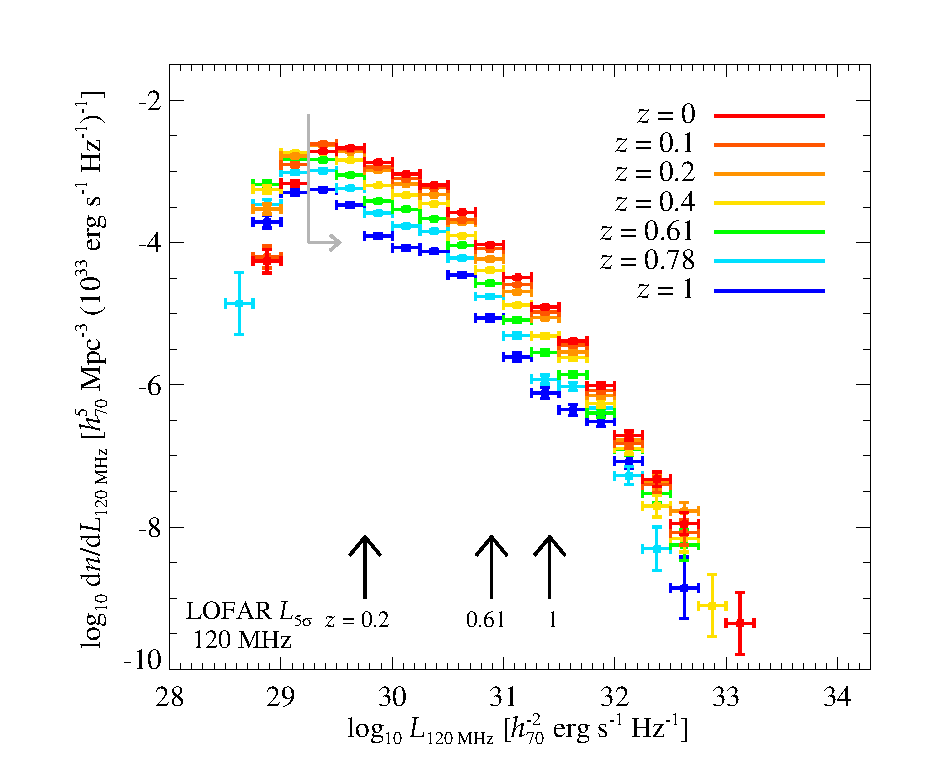
\includegraphics[width=0.5\textwidth,height=0.305\textheight]{figures/RLF_LOFAR.eps}
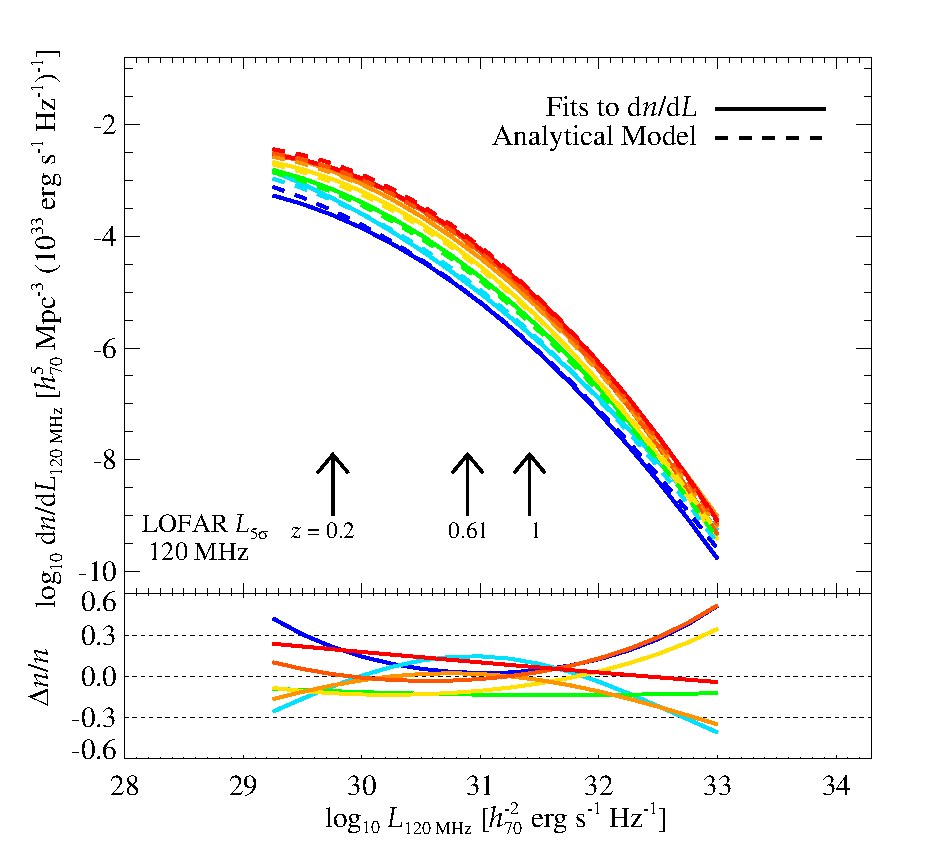
\includegraphics[width=0.47\textwidth,height=0.3\textheight]{figures/RLF_LOFAR_analytical_1.eps}
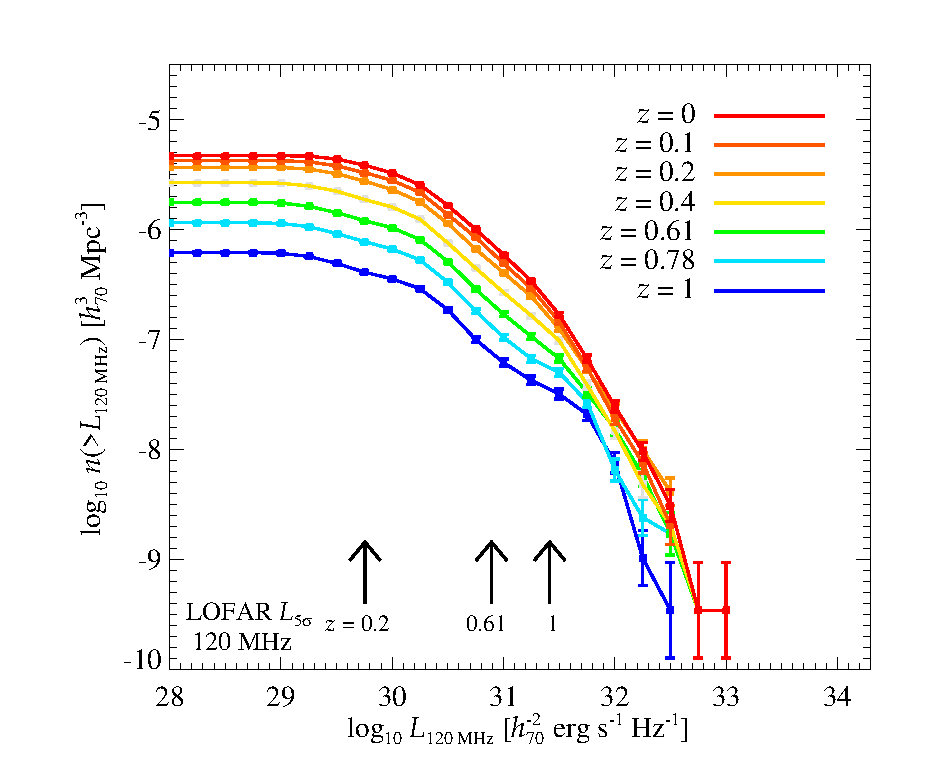
\includegraphics[width=0.5\textwidth,height=0.305\textheight]{figures/CumDensityL_LOFAR.eps}
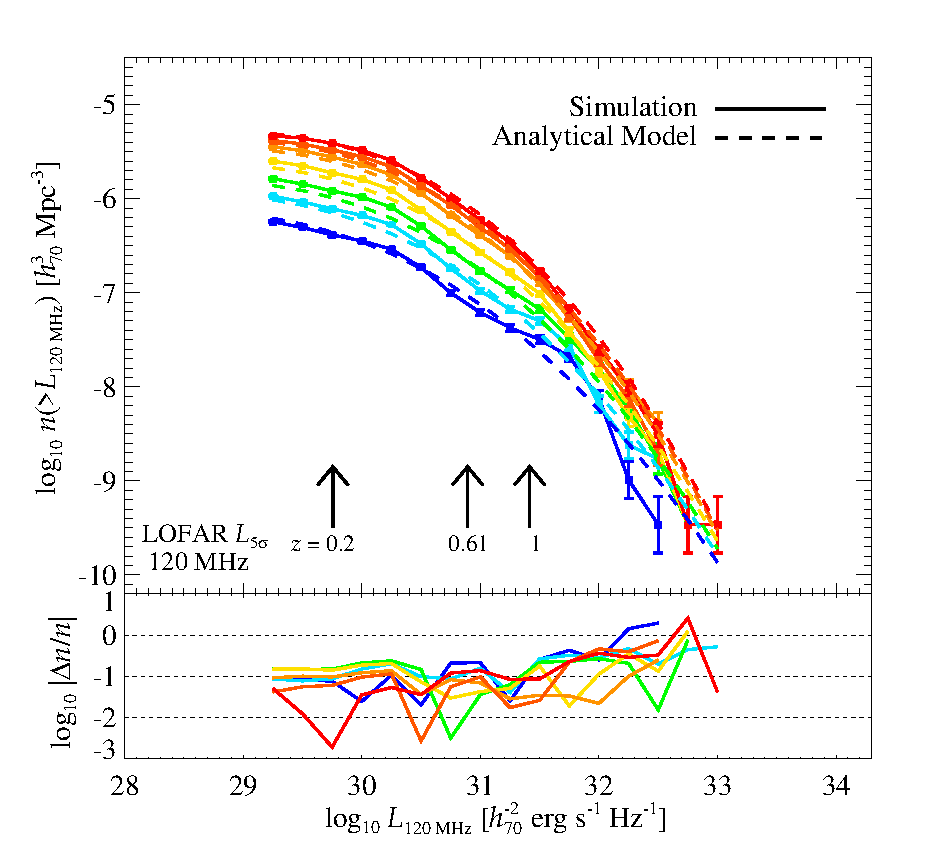
\includegraphics[width=0.47\textwidth,height=0.3\textheight]{figures/CumDensityL_LOFAR_1.eps}
\caption{Radio luminosity function at 120~MHz (top left panel) and cumulative
  number density of RHs (bottom left panel) at different redshifts $z$ (color
  coded) for the model realization described in Section~\ref{sec:4} with a 10\%
  fraction of radio-loud clusters. To obtain an analytical model for $n(L,z)$,
  we fit the RLF at each $z$ with a second-order polynomial and constrain the
  evolution of the three free parameters to follow a power-law function with $z$
  (see main text for details). The right panels show the comparison of the RLF
  fits (top) and the cumulative number density of the MultiDark samples (bottom)
  to the analytical model. The bottom panels of these two panels show the
  relative differences as $\Delta n / n = (n_{\rmn{analytical}} -
  n_{\rmn{fit}})/n_{\rmn{fit}}$. Additionally shown is the LOFAR Tier~1
  \emph{point-source} flux limit of $F_{5\sigma}^{\rmn{PS}}=0.5$~mJy
  \citep{2012JApA..tmp...34R} converted to a luminosity limit at a given
  redshift. Horizontal error bars represent the mass bins while the vertical
  error bars are Poissonian uncertainties.  The light gray line marked by the
  arrow estimates the incompleteness limit owing to the adopted low-mass cut
  (see Section~\ref{sec:2}) and the scatter in the halo luminosities.}
\label{fig:RLF_120}
\end{figure*} 
 
Generally, there is fair agreement between the NVSS RLF and both our modeled RLF
and the RLFs based on observational scaling relations, particularly for
radio-loud fractions between 10\% and 1\%. The RLF obtained from the
$L_{1.4~\rmn{GHz}}-L_{\rmn{X,bol}}$ relation differs from the NVSS RLF at high
luminosities, presumably caused by the large observed scatter. On the other
side, the RLF obtained from the $L_{1.4~\rmn{GHz}}-Y_{\rmn{SZ}}$ relation
matches the NVSS result better. These results need to be consolidated by RLFs
corrected for flux-incompleteness and simulations of larger cosmological volumes
that are more complete at the high-mass end. Figure~\ref{fig:RLF_1.4} shows that
it will be difficult to discriminate between different scenarios at high radio
luminosities (or equivalently masses). Indeed, in the bottom right panel of
Figure~\ref{fig:RLF_1.4} we compare our RLF and the RLFs based on observational
scaling relations for a 10\% fraction of radio-loud clusters to the NVSS
RLF. This suggests that the low-luminosity (low-mass) clusters will be the most
useful in disentangling between different models. This emphasizes the importance
of conducting homogeneous, well controlled surveys of radio halos with the
extended VLA at 1.4 GHz and LOFAR at lower frequencies. Since the latter has
already started to take data, it is extremely timely to present RLF predictions
for this wave length regime of our model.


\subsection{Low-frequency predictions at 120~MHz}

In Figure~\ref{fig:RLF_120}, we show our model predictions at 120~MHz obtained
with the representative realization of our model (as in Sect.~\ref{sec:4}), with
10\% of radio-loud clusters. We show both the differential RLF (top left panel)
and the cumulative number density (bottom left panel) at different redshifts
(corresponding to different MultiDark snapshots of Table~1). Additionally shown
is the expected LOFAR Tier~1 \emph{point-source} flux limit of
$F_{5\sigma}^{\rmn{PS}}=0.5$~mJy \citep{2012JApA..tmp...34R} converted to a
luminosity limit at a given redshift. This flux limit is clearly an
underestimate for nearby RHs, which extend over angular scales of $\sim1$~deg,
as e.g., in the case of the Coma radio halo. In order to make more reliable
predictions, in the following, we will calculate the RH flux limit with
Equation~(10) of \cite{2010A&A...509A..68C}, approximating the halo extension by
$R_{500}$ and requiring the mean flux within the RH half-radius to be higher
than $F_{5\sigma}^{\rmn{PS}}$. This may result in an overestimation of the flux
limit for CCCs, whose radio emission is more centrally concentrated than in
NCCCs. The median $R_{500}$ of our sample is about $0.4$~$h_{70}^{-1}$~Mpc at
all redshifts. This translates to a flux limit of about $30$~mJy at $z = 0.1$,
$7$~mJy at $z = 0.2$ and $0.5$~mJy (equal to the point-source value) at $z
\approx 0.6$.

\begin{figure*}[t]
\centering
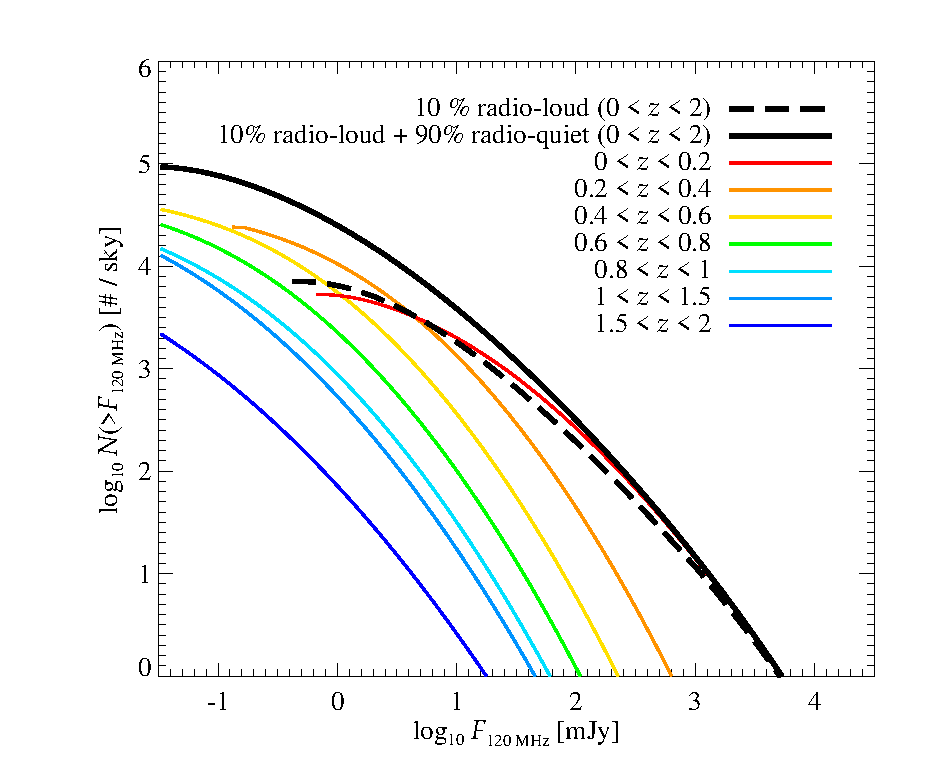
\includegraphics[width=0.48\textwidth]{figures/RLF_LOFAR_flux.eps}
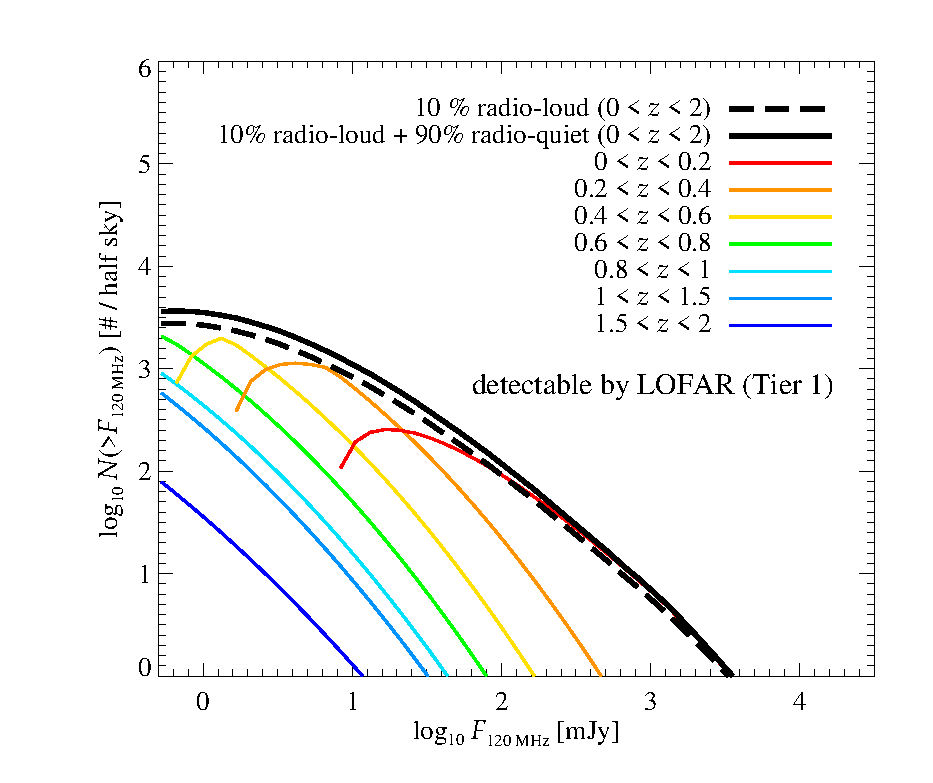
\includegraphics[width=0.48\textwidth]{figures/RLF_LOFAR_flux_detectable.eps}
\caption{Cumulative number of RHs above a certain flux limit in an all-sky
  survey at 120~MHz. We show the result of the model realization described in
  Section~\ref{sec:4} using all cluster and adopting a 10\% fraction of
  radio-loud clusters (black solid thick line) and the result obtained using
  \emph{only} the 10\% radio-loud clusters (black dashed thick line). We also
  show the differential contribution to the total RLF in redshift slices. Note
  that the total number of (detectable) RHs would be dramatically reduced by the
  presence of a break in the model at some low luminosity-scale, or a
  mass-dependence of the model parameters causing the RH luminosities to
  decrease at low masses.  \emph{Left.} Total number of RHs in the sky.
  \emph{Right.} Number of detectable RHs by LOFAR Tier~1 survey considering its
  sky coverage (half sky) and adopting a realistic flux limit corresponding to
  different angular source extensions at different redshifts. The lower flux
  limit is taken to be $F_{5\sigma}^{\rmn{PS}}=0.5$~mJy (see main text for
  details).  }
\label{fig:RLF_120_flux}
\end{figure*}

%% corrected until here

In order to make a more quantitative prediction, we build an analytical model to
describe the evolving RLF. We fit the 120~MHz RLF at different redshifts as a
2-order polynomial function in the form of $\log_{10}
\rmn{d}n/\rmn{d}L_{120~\rmn{MHz}} = A_{1} + A_{2}~\log_{10} L_{120~\rmn{MHz}} +
A_{3}~(\log_{10} L_{120~\rmn{MHz}})^{2}$ (only luminosities higher then
$\log_{10} L_{120~\rmn{120MHz}} \geq 29.25$ are used in order to exclude the
artificial low-luminosity decrease). We then obtain an analytical form for the
dependence of the three parameters $A_{i}$ with respect to the redshift as
$A_{i} = A_{i,0} + A_{i,1}~(1+z)$.\footnote{The values of these parameters are
  $A_{1,0} = -436.79$, $A_{1,1} = 109.75$, $B_{1,0} = 29.68$, $B_{1,1} = -7.17$,
  $C_{1,0} = -0.51$ and $C_{1,1}$ = 0.12, and units are as the top left plot of
  Figure~\ref{fig:RLF_120}.} In the right panels of Figure~\ref{fig:RLF_120}, we
compare the RLF fits (top) and the cumulative number density (bottom) to the
result obtained with the derived analytical model. The results obtained with the
latter well compare with the prediction at a given redshift showing a
significant deviation only at very high luminosities, and at very low
luminosities for the highest considered redshifts, where however the very small
statistic significantly affects the result.

This analytical model describing $\rmn{d}N^2(L,z)/\rmn{d}V_{\rmn{C}}\rmn{d}L$, where $V_{\rmn{C}}$ is the comoving volume, is then used to calculate the total cumulative number of RHs in the sky above a given flux value $F$ as
%
\begin{equation}
N(>F)  =  \int_{z_1}^{z_2} \rmn{d}z \frac{\rmn{d}V_{\rmn{C}}}{\rmn{d}z} \int_{L(F)}^{\infty} \frac{\rmn{d}N^2(L,z)}{\rmn{d}V_{\rmn{C}}\rmn{d}L} \rmn{d}L \, ,
\label{eq:NtotRH}
\end{equation}
%
where $L(F) = 4 \pi D(z)^2 F$ and $D(z)$ is the luminosity distance computed from the corresponding redshift $z$.
The result is shown in the left panel of Figure~\ref{fig:RLF_120_flux}. We show the particular realization of our model described in the previous section with 10\% fraction of radio-loud clusters (black solid thick line; only luminosities above $\log_{10} L_{120~\rmn{120MHz}} \geq 29.25$ are integrated). The total is obtained integrating up to $z_{2} = 2$ as above this value only few clusters survive our mass cut and none would be detectable. The lower redshift limit (indicated as 0 in Figure~\ref{fig:RLF_120_flux}) is $z_{1} = 0.018$ as the closer known RH, i.e.~Perseus. We also show how the total result builds up in different redshift bins. We contrast this with the RH total cumulative number obtained using \emph{only} the 10\% radio-loud clusters (black dashed thick line; this is done constructing the corresponding RLF and repeating the above steps to build an analytical model, where only luminosities above $\log_{10} L_{120~\rmn{120MHz}} \geq 30.75$ are integrated). 
%We additionally shown the two total results scaled down by a $50\%$ to roughly mimic an eventual RH redshift evolution as a consequence of a higher inverse Compton energy loss on the CMB for higher redshift (\citealp{2002A&A...396...83E}; this is somehow conservative as most of our cluster magnetic fields are comparable or higher than the CMB magnetic field). 

In the right panel of Figure~\ref{fig:RLF_120_flux}, we show the total number of RHs that would be \emph{detectable} by the LOFAR Tier~1 survey, where its sky coverage (about half sky) is taken into account. This is calculated with Equation~(\ref{eq:NtotRH}) taking $F = F_{\rmn{min}}$ where $F_{\rmn{min}}$ is calculated with the Equation~(10) of \cite{2010A&A...509A..68C} as explained above. The lower flux limit is taken to be $F_{5\sigma}^{\rmn{PS}}$, meaning that when $F_{\rmn{min}} < 0.5$~mJy, i.e.~at redshift above approximately $z = 0.6$, it is fixed at 0.5~mJy.  

LOFAR Tier~1 at 120~MHz should be able to detect a total of about $3500$ clusters hosting RHs above 0.5~mJy. The precise number is strongly dependent on the underling assumptions. There are two main uncertainties in our model: the fraction of radio-loud to radio-quiet clusters and the corresponding relative normalization (which in turn is the result of the interplay of the $\gamma_{\rmn{th}}$, $B_{0}$, $\alpha_{B}$, $g_{\rmn{CR}}$, and therefore $X_{CR}$, parameters). The first is relevant only at medium-high luminosities, as can be seen from the 1.4~GHz RLFs in the top left panel of Figure~\ref{fig:RLF_1.4}, and therefore would not dramatically impact the total number of (detectable) RHs because this is dominated by the low luminosities. We asses the second uncertainty by comparing the total result of our model (black solid line) with the RLF obtained only from the radio-loud population (black dashed line). Their difference somehow shows the uncertainty in the modeling for a fixed fraction of radio-loud clusters as all the configuration between the solid and dashed lines can be virtually realized changing the relative normalization of the loud and quiet populations. 

The total number of (detectable) RHs is expected to be quite high. This is mainly due to neglecting an eventual mass-dependence in the model parameters and, more importantly, to the assumption that the model holds down to masses of about $M_{200}\approx1.4\times10^{14}$~$h_{70}^{-1}$~M$_{\odot}$ without any break. In fact, looking at the radio-to-X-ray and radio-to-SZ scaling relations of Figure~\ref{fig:PLSZ}, we can see that most of the RHs in our sample, also for the radio-loud population, lie at low masses and therefore at low luminosities unproved by current observations. The presence of a break at some low mass-scale, or some sort of mass-dependence in the model parameters causing a lowering of the RH luminosities, would eventually result in a dramatically reduced number of total (detectable) RHs. This would be in better agreement with recent predictions of a few to hundreds observable RHs by e.g.~\cite{2010A&A...509A..68C} and \cite{2011arXiv1110.2786S}, while \cite{2002A&A...396...83E} also found that thousands of RHs would be detectable by future surveys. However, current information do not permit to make any reliable assumption in this sense. 

Another relevant issue in such surveys is the identification of RHs and their hosting clusters (see also \citealp{2010A&A...509A..68C}). RHs constitute a small part of the entire radio source population and therefore need to be distinguished from the emission produced by other sources. A good approach in this sense is to use X-ray samples of galaxy clusters. This underlines the importance of the future eROSITA mission also for the cluster non-thermal emission study as it is expected to detect around $10^{5}$ clusters up to redshift $z \approx 1.3$ (see e.g.~\citealp{2011MSAIS..17..159C}).

Our results show the potentiality of the LOFAR survey, and other future radio instruments, in determining the (120~MHz) RLF properties in a very broad range of luminosities. In particular, it should permit a robust determination of the number of clusters hosting RHs at a given luminosity (mass). This will be extremely helpful in determining the parameter values for our hadronic model and eventually in elucidating the RH generation mechanism.


%%%%%%%%%%%%%%%%%%%%%%%%%%%%%%%%%%%%%%%%%%%%%%%%%%%%%%%%%%%%%%%%%%%
%%%%%%%%%%%%%%%%%%%%%%%%%%%%%%%%%%%%%%%%%%%%%%%%%%%%%%%%%%%%%%%%%%%
\section{Conclusions}
\label{sec:6}
We present predictions for the RH population assuming that RHs are generated by secondaries of the hadronic CR interactions with the ICM. We construct a complete cosmological sample of galaxy clusters from the MultiDark N-body simulation \citep{2011arXiv1104.5130P} using seven snapshots from $z = 0$ up to $z = 1$. We select galaxy clusters imposing a low mass cut at $M_{200}\approx1.4\times10^{14}$~$h_{70}^{-1}$~M$_{\odot}$. 

We first construct a \emph{phenomenological} model, based on the observed REXCESS cluster gas profiles \citep{2008A&A...487..431C} and cluster mass-to-gas fraction relation \citep{2009ApJ...693.1142S}, which assigns a ICM gas density to a DM halo given only its total mass. In this way, we obtain a cosmological complete mock catalog of galaxy clusters matching the observed $L_{\rmn{X, bol}}$-to-mass, $Y_{\rmn{X}}$-to mass and $Y_{\rmn{SZ}}$-to-mass relations, and the X-ray luminosity function.

We then construct a new \emph{hybrid} hadronic model for the CR distribution in clusters. We merge previous results from simulations and analytical works. We adopt the semi-analytical mass-dependent universal normalization CR profile obtained from the hydrodynamic cluster cosmological simulations of \cite{2010MNRAS.409..449P}. We merge this with the analytical model of \cite{2011A&A...527A..99E} which includes the treatment of CR transport processes. While CR advection tends to result in centrally enhanced CR profiles, the propagation in form of CR streaming and diffusion tends to produce flat CR profiles. The latter phenomena were not considered in previous works for sake of simplicity but turn out to be dramatically important. Note that the choice to adopt the \cite{2010MNRAS.409..449P} simulation-derived universal profile, providing a mass-scaling, may introduce an overcooling problem. This can be counteracted by changing the $\gamma_{\rmn{tu}}$ and $\alpha_B$ values, governing the CR transport processes and the magnetic field radial decline, respectively. However, the risk is that, when modeling a given galaxy cluster, the final $\gamma_{\rmn{tu}}$ value may be biased as the CR transport effects are degenerate with the initial CR profile, the $\alpha_B$ value, and other possible effects not considered here as cluster asphericity and the contribution of primary electrons accelerated in outer shocks. Additionally, by adopting the result of \cite{2010MNRAS.409..449P}, which is parametrized with three CR spectral indexes $\alpha_{i}=(2.55,2.3,2.15)$, we are also neglecting the possible CR transport effects on the CR spectral index (see \citealp{2011A&A...527A..99E} for details). 

We model the Coma and Abell~2163 giant radio halos, and the Perseus and Ophiuchus radio mini-halos at 1.4~GHz. Our hybrid hadronic model can reproduce the surface brightness both of giant and mini-halos, solving problems of the \emph{classical} hadronic model, and we recover the total radio luminosity within maximum of 20\%. We do not find any tension with existing observations and constraints, particularly on magnetic field values. Note that radio measurements put stringent constraints than corresponding gamma-ray observations, with the exception of the Coma cluster case. Gamma-ray measurements are fundamental to disentangle between the hadronic and re-acceleration models. The results presented here show however that gamma-ray predictions should be scaled down with respect to previous works (e.g.~at least a factor of two for Perseus with respect to \citealp{2010MNRAS.409..449P}). Note in fact that the parameter space of the new hybrid hadronic model constructed here is largely extended with respect to previous models.

We then calculate the radio emission of the clusters of the mock catalog and show how different parameter choices in the CR modeling may affect the final result. We select a representative realization of our CR model and compare it with existing observations. Thanks to the inclusion of the CR transport phenomena, the hadronic model can now reproduce the apparent cluster bimodality observed in the radio-to-X-ray scaling relation \citep{2009A&A...507..661B,2011A&A...527A..99E}. At the same time, we can also reproduce the radio-to-SZ scaling relation recently presented by \cite{2012MNRAS.421L.112B} which does not show any evidence of bimodality. This discrepancy may be only apparent as we can reproduce both results.

We calculate the 1.4~GHz RLF and compare it with the observed one \citep{1999NewA....4..141G} finding a good agreement. The comparison between different RLFs illustrates that the low luminosity (mass) regime is the most promising range where to constrain different models by clearly determining the RH fraction against the total galaxy cluster population. We therefore calculate the 120~MHz RLF and cumulative number density, and make prediction for the LOFAR cluster survey. We compute the total cumulative number of RHs above a certain flux limit and show that, under our assumptions, we would expect LOFAR Tier~1 at 120~MHz to detect about ~3500 RHs above 0.5~mJy. The precise number is strongly dependent on the underling assumptions and, in particular, to the assumption that the model holds down to masses of about $M_{200}\approx1.4\times10^{14}$~$h_{70}^{-1}$~M$_{\odot}$ without any break. Most of the RHs in our sample lie at low masses and therefore at low luminosities unproved by current observations. The presence of a break at some low mass-scale, or some sort of mass-dependence in the model parameters causing a lowering of the RH luminosities, would eventually result in a dramatically reduced number of total (detectable) RHs. As the current available information do not permit to make any reliable assumption in this direction, we have to wait for the LOFAR results to shed light on this issue. 

We show the potentiality of observations by LOFAR, and other next-generation low-sensitivity radio instruments, in determining the RLF properties in a very broad range of luminosities. In particular, they should permit a robust determination of the number of clusters hosting RHs at a given luminosity (mass) and therefore elucidate the relation of the radio emission with cluster dynamical states in synergy with future X-ray missions like eROSITA. This will be extremely helpful in determining the parameter values for our hadronic model and eventually in elucidating the RH generation mechanism.

Concluding, we want to underline that thanks to our gas profile \emph{phenomenological} model and the new \emph{hybrid} hadronic model, we can provide cosmological complete multi-frequency cluster mock catalogs at different redshifts reproducing current observations. These can be used for different scientific purposes. We will make these catalogs, containing among others the $\rho_{\rmn{gas}}$, $L_{\rmn{X, bol}}$, $Y_{\rmn{X}}$, $Y_{\rmn{SZ}}$, $L_{120~\rmn{GHz}}$, $L_{1.4~\rmn{GHz}}$ and $L_{\gamma}$ values, freely available on-line.


%%%%%%%%%%%%%%%%%%%%%%%%%%%%%%%%%%%%%%%%%%%%%%%%%%%%%%%%%%%%%%%%%%%
%%%%%%%%%%%%%%%%%%%%%%%%%%%%%%%%%%%%%%%%%%%%%%%%%%%%%%%%%%%%%%%%%%%
\begin{acknowledgements}
We would like to thank Anders Pinzke for his invaluable help with the formulae and for many useful discussions. We also thanks Gustavo Yepes, Jos\'e Alberto Rubi\~no, Frazer Pearce, Andrey Kravtsov, Harald Ebeling, Miguel-Angel Perez Torres and Adam Mantz for the useful discussions and advices. We would also like to thank Matteo Murgia for kindly providing the radio surface brightness profiles of Ophiuchucs and Abell~2163, and Wolfgang Reich for providing the radio map of Coma. {\bf Thanks MultiDark database guys, etc.}.
BLA BLA BLA\\ 
F.~Z.~acknowledges the CSIC financial support as a JAE-Predoc grant of the program ``Junta para la Ampliaci\'on de Estudios'' co-financed by the FSE.
\end{acknowledgements}


%%%%%%%%%%%%%%%%%%%%%%%%%%%%%%%%%%%%%%%%%%%%%%%%%%%%%%%%%%%%%%%%%%%
%%%%%%%%%%%%%%%%%%%%%%%%%%%%%%%%%%%%%%%%%%%%%%%%%%%%%%%%%%%%%%%%%%%
\bibliographystyle{aa}
\bibliography{bib_file}


%%%%%%%%%%%%%%%%%%%%%%%%%%%%%%%%%%%%%%%%%%%%%%%%%%%%%%%%%%%%%%%%%%%
%%%%%%%%%%%%%%%%%%%%%%%%%%%%%%%%%%%%%%%%%%%%%%%%%%%%%%%%%%%%%%%%%%%
\begin{appendix}

\section{Cosmic Rays Modeling Details}
\label{app:B}

Here, we describe how our final \emph{hybrid} model for CRs of Section~\ref{sec:2.3} has been built. 
Following closely \cite{2011A&A...527A..99E}, when turbulent advection
completely dominates, the CR normalization can be expressed as in 
Equation~(\ref{eq:Csimple_1}). However, both propagation and advection shape the 
CR profile. This is analytically developed by solving the continuity equation for CRs 
and obtaining the CR density profile $\rho_{\rmn{CR}}$ of Equation~(\ref{eg:rhoCR_1}). 
Assuming for simplicity that $P(R)/P_{0}=n_{\rmn{e}}(R)/n_{0}$, so neglecting the 
temperature dependence, with a standard $\beta$-profile for the electron density,

\begin{equation}
n_{\rmn{e}} = n_{0} \left( 1+\frac{R^{2}}{R_{\rmn{c}}^{2}} \right)^{-\frac{3\beta_{\rmn{cl}}}{2}} \, ,
\label{eq:beta_profile}
\end{equation} 

the solution of Equation~(\ref{eg:rhoCR_1}) is physical only for $\rho_{\rmn{CR}}$ between

\begin{equation}
R_{\pm} = \frac{3\beta_{\rmn{cl}}}{2\gamma}R_{*}\left(1\pm\sqrt{1-\left(\frac{2R_{\rmn{c}}\gamma}{3\beta_{\rmn{cl}}R_{*}}\right)^{2}}\right) \, ,
\label{eq:Rpm}
\end{equation} 

while it is non-stationary outside these radii where we just set $\rho_{\rmn{CR}}(R) = \rho_{\rm{CR}}(R_{\pm})$
for $R > R_{+}$ and $R < R_{-}$, respectively. We refer the reader to \cite{2011A&A...527A..99E} for 
further details. Eventually, the final CR normalization profile, 
$C(R)=C_{0}(\rho_{\rmn{CR}}(R)/\rho_{\rmn{CR},0})^{\beta_{\rmn{CR}}}$, results to be

\begin{equation}
C(R) = C_{0}\left( 1+ \frac{R^{2}}{R_{C}^{2}} \right)^{-\beta_{\rmn{c}}} \rmn{exp}\left( {\frac{R}{R_{*}}\beta_{\rmn{CR}}} \right)
\label{eq:Ctransport}
\end{equation} 

for $R_{-}<R<R_{+}$, where $\beta_{\rmn{c}}=3\beta_{\rmn{cl}}~\beta_{\rmn{CR}}/2\gamma$, 
and $C(R) = C(R_{\pm})$ for $R<R_{-}$ and $R>R_{+}$, respectively. Therefore, we can 
mimic different CR transport cases varying the value of the transport parameter 
$\gamma_{\rmn{tu}}$. For a high $\gamma_{\rmn{tu}}$ value, we fall in the 
advection-dominated case, while the CR profile is flat when $\gamma_{\rmn{tu}} \sim1$ \citep{2011A&A...527A..99E}. 

In Figure~\ref{fig:simpleVStransport}, we show a comparison between $C_{\rmn{adv}}$ of 
Equation~(\ref{eq:Csimple_1}) and $C$ of Equation~(\ref{eq:Ctransport}) considering the 
NCCC Coma and CCC Perseus cases. While for Coma we adopt the $\beta$-profile of 
\citet{1992A&A...259L..31B}, Perseus needs a double-$\beta$ profile. We adopt both the 
approximation $P(R)/P_{0}=n_{\rmn{e}}(R)/n_{0}$ and the proper Perseus pressure profile 
(X-ray data from \citealp{2003ApJ...590..225C}). Note that the \cite{2011A&A...527A..99E} 
formalism is exact only for the approximation $P(R)/P_{0}=n_{\rmn{e}}(R)/n_{0}$ where $n_{\rmn{e}}$ 
is a $\beta$-profile. Nevertheless, we adopt the above formulae also for Perseus as a good approximation, 
i.e.~we adopt $C(R)=C_{0}(\rho_{\rmn{CR}}(R)/\rho_{\rmn{CR},0})^{\beta_{\rmn{CR}}}$
within $R_{\pm}$ of Equation~(\ref{eq:Rpm}), and $C(R) = C(R_{\pm})$ for $R > R_{+}$ 
and $R < R_{-}$, respectively; we take $R_{\rmn{c}}$ in Equation~(\ref{eq:Rpm}) to be equal to the Perseus 
double-$\beta$ profile outer core radius and fix $\beta_{\rmn{cl}}=0.8$. The relevant 
parameters are $\gamma_{\rmn{tu}}$ and the exponential factor of Equation~(\ref{eg:rhoCR_1}). 
In fact, as we will se in the following, the two radii $R_{\pm}$ are not critically affected 
by the detail of $\eta(R)$. Therefore, despite the approximation, this approach captures the 
main CR transport effects also for the Perseus case. 

In Figure~\ref{fig:simpleVStransport}, we additionally show the result in case 
$C(R)=C_{\rmn{semi-analytical}}(R)=\tilde{C}(R)\rho_{\rmn{\rmn{gas}}}(R)/m_{\rmn{p}}$ 
where $\tilde{C}(R)$ is the universal normalization CR profile found in cosmological 
simulations \citep{2010MNRAS.409..449P}. As expected, the CR profile driven by 
simulations is characterized by a more centrally peaked profile with respect to the 
analytical case. Note also the flatter profile of Coma with respect to Perseus, which 
reflects their NCCC and CCC classification, respectively. Finally, the effect of varying 
the turbulent cluster state by means of $\gamma_{\rmn{tu}}$ can be clearly appreciated.

\begin{figure*}[t!]
\centering
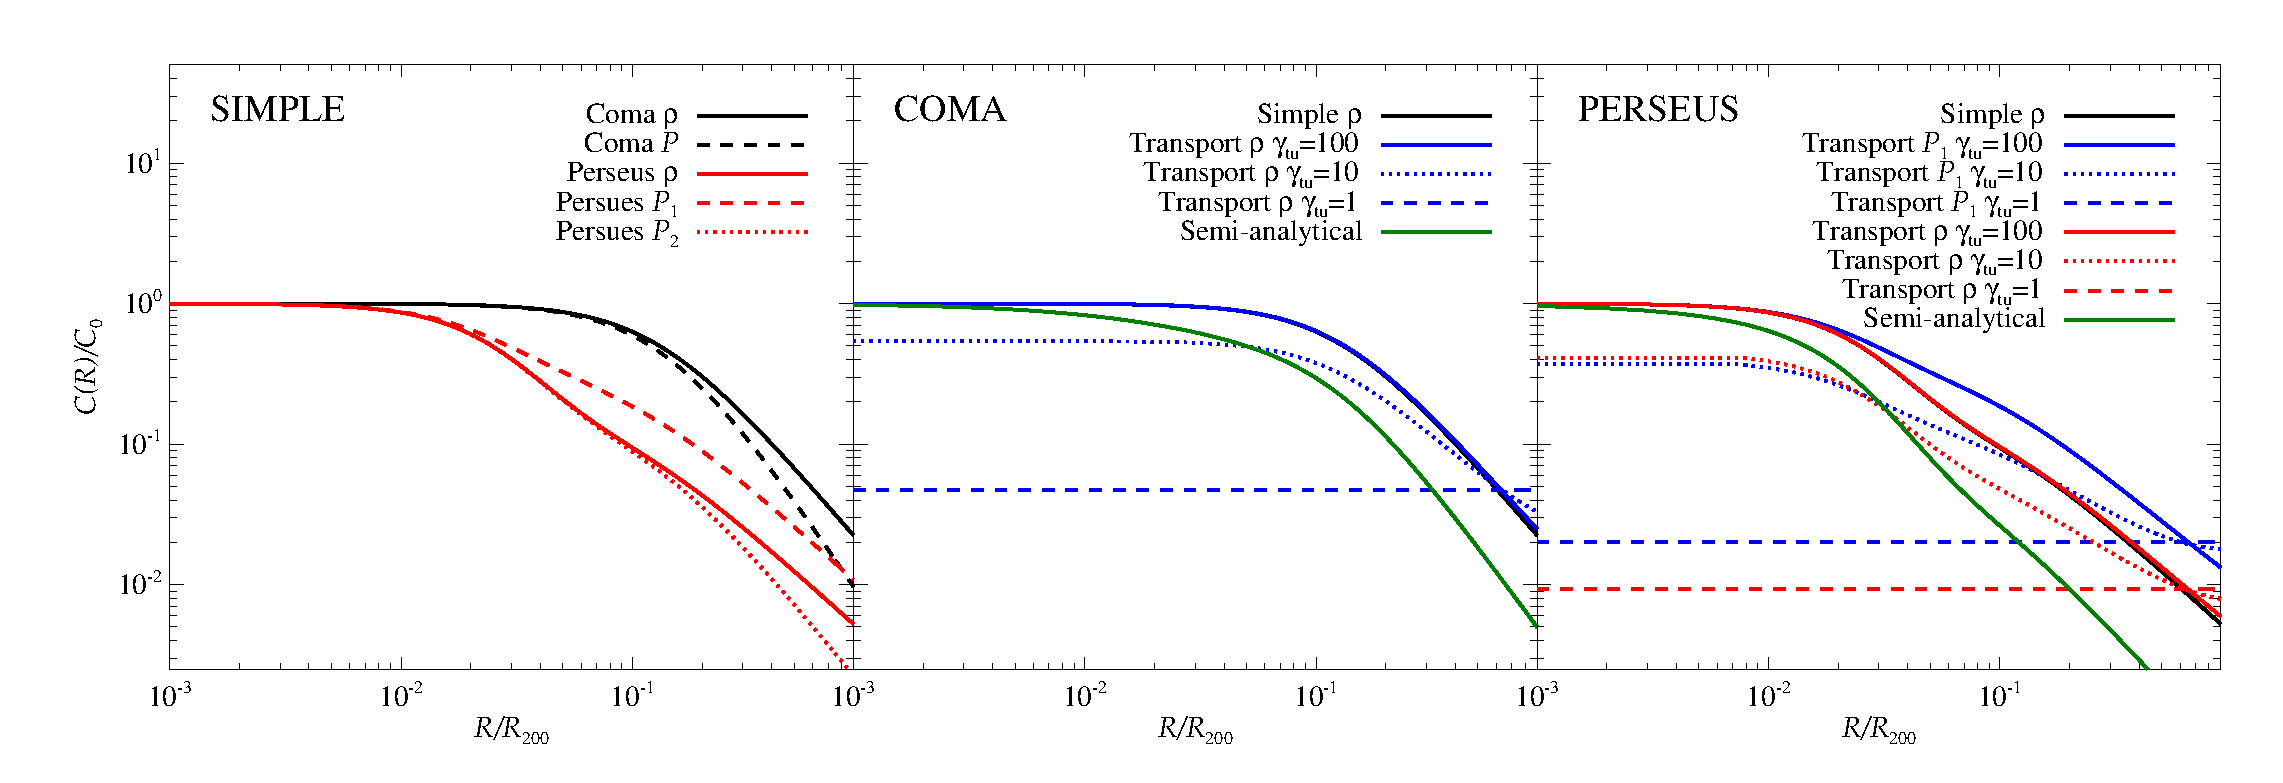
\includegraphics[width=0.99\textwidth]{figures/CR_profiles_simple_comparison.eps}
\caption{Comparison of different CR profiles. The left plot shows the \emph{simple} advective $C_{\rmn{adv}}$ of Equation~(\ref{eq:Csimple_1}) for the Coma and Perseus cases both neglecting the temperature dependence ($\rho$) and considering it ($P$). The temperature profile of Coma has been modified so that it follows the characteristic decline toward the cluster periphery. Perseus is a CCC and it is characterized by a central dip in the temperature profile which may importantly affect the final CR profile, so we adopt the temperature profile as given in \cite{2003ApJ...590..225C} ($P_{1}$). We also show the case where we only apply the characteristic decline toward the cluster periphery ($P_{2}$). The other two right plots show the \emph{transport} case of Equation~(\ref{eq:Ctransport}) for Coma and Perseus for different values of $\gamma_{\rmn{tu}}$ in comparison with the \emph{simple} case. Additionally shown is the result in case of $C(R)=C_{\rmn{semi-analytical}}(R)=\tilde{C}(R)\rho_{\rmn{gas}}(R)/m_{\rmn{p}}$ where $\tilde{C}(R)$ is the mass-dependent universal normalization CR profile found in cosmological simulations \citep{2010MNRAS.409..449P}. The \emph{simple} and \emph{semi-analytical} profiles are normalized at $C_{0}=C(0)$. The transport cases are normalized at $C_{0}=C(0,\gamma_{\rmn{tu}}=100)$, where we fix the CR populations to have a constant total CR number as in Equation~(36) of \cite{2011A&A...527A..99E} integrating up $R_{200}$. We adopt $\alpha=2.3$.}
\label{fig:simpleVStransport}
\end{figure*}

We want now to generalize the \cite{2011A&A...527A..99E} approach to our GNFW 
gas profiles of Section~\ref{sec:2.2}, in addition to the universal temperature drop in
the cluster outskirts, and merge it with the $\tilde{C}$ universal CR normalization 
obtained from simulations. Adopting our profile 
$C_{\rm{hybrid}} = \tilde{C}(R) \frac{\rho_{\rmn{gas}}(R)}{m_\rmn{p}} \frac{T(R)}{T_0} $
into Equation~(\ref{eq:eta}), there is not an analytical solution for Equation~(\ref{eg:rhoCR_1}) 
as in \cite{2011A&A...527A..99E}. This results in a 5-order equation; a numerical 
solution would not be of practical use for our large MultiDark sample. For simplicity, we 
proceed as in the Perseus case, adopting the above formulae after some convenient 
modifications detailed in the following. 

In the case of $P(R)/P_{0}=n_{\rmn{e,GNFW}}(R)/n_{0}$, with $n_{\rmn{e,GNFW}}$ given by Equation~(\ref{eq:gnfw}), 
there exist an exact analytical solution following the \cite{2011A&A...527A..99E} treatment. Therefore, in order 
to evaluate the systematic error that we are introducing with the above described approach, 
in Figure~\ref{fig:REXexactVSfake}, we compare $C(R)$ of the GNFW exact solution and the approximate 
case where we use the \cite{2011A&A...527A..99E} formulae adopting $P(R)/P_{0}=n_{\rmn{e,GNFW}}(R)/n_{0}$. 
In the second case, we fix $R_{-}=10^{-3}R/R_{200}$ to mimic the typical $R_{-}$ value of the exact solution, otherwise 
an unphysical step feature would appear at $\leq10^{-2}R/R_{200}$. This latter approximation is kept in the final hybrid 
model; note however that this does not change at all the model surface brightness and total luminosity. 
As clear from Figure~\ref{fig:REXexactVSfake}, there is almost no difference between the two cases. 
This shows that the approximated approach strategy can be safely followed in order to derive a fully working model 
capturing the main CR transport effects. 

Summarizing, $C_{hybrid}$ of Equation~(\ref{eq:Cf}) defines our final hybrid CR normalization profile which is 
$C(R)=C_{0}(\rho_{\rmn{CR}}(R)/\rho_{\rmn{CR},0})^{\beta_{\rmn{CR}}}$ within $R_{\pm}$ of Equation~(\ref{eq:Rpm}), 
and $C(R) = C(R_{\pm})$ for $R > R_{+}$ and $R < R_{-}$, respectively. Note that in our final formulation, 
$R_{\rmn{c}}$ of Equation~(\ref{eq:Rpm}) becomes the characteristic radius of our GNFW gas profile of 
Section~\ref{sec:2.2}, i.e.~$R_{\rmn{c}} = 0.2 R_{500}$, and $\beta_{\rmn{cl}}=0.8$ 
(we checked that varying the value of $\beta_{\rmn{cl}}$ between 0.4 and 1.2 has no impact at all).

\begin{figure}[t!]
\centering
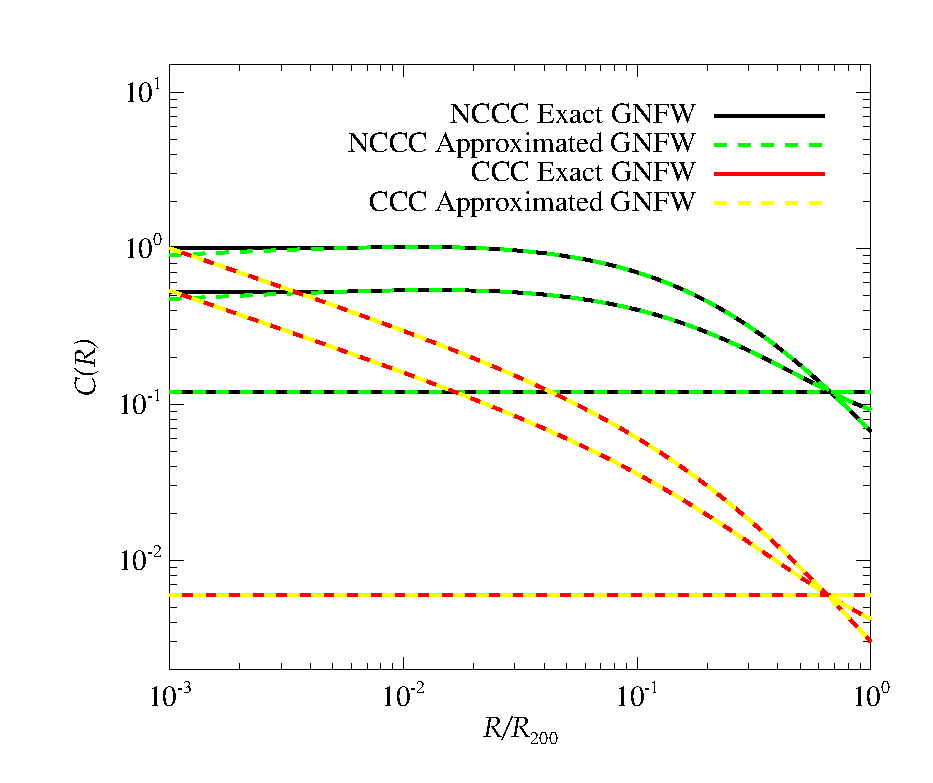
\includegraphics[width=0.5\textwidth]{figures/CR_profiles_REXexactVSfake.eps}
\caption{Comparison of $C(R)$ for the GNFW exact solution and the approximated case where we use the \cite{2011A&A...527A..99E} formulae with $P(R)/P_{0}=n_{\rmn{e,GNFW}}(R)/n_{0}$. Both the NCCC and CCC cases for the respective GNFW profiles derived in Section~\ref{sec:2.2} are shown. From top to bottom: $\gamma_{\rmn{tu}}=100$, $\gamma_{\rmn{tu}}=10$ and $\gamma_{\rmn{tu}}=1$. The normalization is done at $C_{0}=C(0,\gamma_{\rmn{tu}}=100)$ of the exact model where we fix the CR populations to have a constant total CR number as in Equation~(36) of \cite{2011A&A...527A..99E} integrating up $R_{200}$. Note that the $C(0,\gamma_{\rmn{tu}}=100)$ value for the CCC case is identical between the exact and approximated model, while there is a small difference of about 9\% in the NCCC case. We adopt $\alpha=2.3$.}
\label{fig:REXexactVSfake}
\end{figure}


%%%%%%%%%%%%%%%%%%%%%%%%%%%%%%%%%%%%%%%%%%%%%%%%%%%%%%%%%%%%%%%%%%%
%%%%%%%%%%%%%%%%%%%%%%%%%%%%%%%%%%%%%%%%%%%%%%%%%%%%%%%%%%%%%%%%%%%

\section{Radio Emission Calculation}
\label{app:A}

The factor $A_{\nu}$ for the synchrotron radio luminosity calculation of Equation~(\ref{eq:jnu}) is (see also \citealp{2008MNRAS.385.1211P} and \citealp{2011A&A...527A..99E})

\begin{equation}
A_{\nu} = A_{\rmn{E_{synch}}} \frac{16^{2-\alpha_{\rmn{e}}}\sigma_{\rmn{pp}}m_{\rmn{e}}c^{2}}{(\alpha_{\rmn{e}}-2)\sigma_{\rmn{T}}\epsilon_{B_{\rmn{C}}}m_{\rmn{p}}}\left(\frac{m_{\rmn{p}}
}{m_{\rmn{e}}}\right)^{\alpha_{\rmn{e}}-2} \left(\frac{m_{\rmn{e}}c^{2}}{\rmn{GeV}}\right)^{\alpha_{\rmn{e}}-1} \, ,
\end{equation}

with

\begin{equation}
A_{\rmn{E_{synch}}} = \frac{\sqrt{3\pi}}{32\pi}\frac{B_{\rmn{c}}e^{3}}{m_{\rmn{e}}c^{2}}\frac{\alpha_{\rmn{e}}+\frac{7}{3}}{\alpha_{\rmn{e}}+1}\frac{\Gamma\left(\frac{3\alpha_{\rmn{e}}-1}{12}\right)\Gamma\left(\frac{3\alpha_{\rmn{e}}+7}{12}\right)\Gamma\left(\frac{\alpha_{\rmn{e}}+5}{4}\right)}{\Gamma\left(\frac{\alpha_{\rmn{e}}+7}{4}\right)} \, ,
\end{equation}

where $\alpha_{\rmn{e}}=\alpha+1$, the effective inelastic cross-section for proton-proton interactions $\sigma_{\rmn{pp}} = 32~(0.96+\rmn{e}^{4.42-2.4\alpha})$, $B_{\rmn{c}} = \sqrt{ 8 \pi \epsilon_{B_{\rmn{c}}}} \simeq 31 \left( \frac{\nu}{\rmn{GHz}} \right)~\mu$G, and $\Gamma$ is the Gamma-function \citep{1965hmfw.book.....A}. $A_{\rmn{E_{synch}}}$ is expressed in erg, and $A_{\nu}$ is expressed in erg~cm$^{3}$~g$^{-1}$~sr$^{-1}$. 


%The dimension of $A_{\rmn{E_{synch}}}$ is [erg] if the electron charge $e$ is expressed in [ues], the electron mass $m_{\rmn{e}}$ in [g], the speed of light $c$ in [cm/s] and the critical magnetic field value $B_{\rmn{c}}$ in [G]. The dimension of $A_{\nu}$ is [erg~cm$^{3}$~g$^{-1}$~sr$^{-1}$] if the effective inelastic cross-section for proton-proton interactions $\sigma_{\rmn{pp}} = 32~(0.96+\rmn{e}^{4.42-2.4\alpha})$ and the Thomson cross-section $\sigma_{\rmn{T}}$ are expressed in [mbarn], the first $m_{\rmn{e}}$ in [g], the first $c$ in [cm/s], $B_{\rmn{c}}$ of $\epsilon_{B_{\rmn{C}}}$ is expressed in [G] and $m_{\rmn{p}}$ in [g]. 
%Pay attention that here the $B_{C}$ value must be expressed in [G] to get the correct final units while in the main text it is expressed in [$\mu$G] because there it cancels out with the other magnetic field values.  

The generalization of the radio luminosity calculation to three CR spectral indexes and the inclusion of the normalization parameter $g_{\rmn{CR}}$, following \cite{2010MNRAS.409..449P}, changes $j_{\nu}$ into

\begin{eqnarray}
j_{\nu,\rmn{hybrid}} & = &g_{\rmn{CR}} C(R) \rho_{\rmn{gas}}(R) \frac{\epsilon_{\rmn{B}}(R)}{\epsilon_{\rmn{B}}(R)+\epsilon_{\rmn{CMB}}} \nonumber \\
& \times & \Sigma_{i=1}^{3} \Delta_{i} A_{\nu,i} \left( \frac{\epsilon_{\rmn{B}}(R)}{\epsilon_{B_{\rmn{c}}}} \right)^{\frac{\alpha_{i}-2}{4}}  \, ,
\end{eqnarray}

where the sum is over the three CR spectral indexes $\alpha_{i}=(2.55,2.3,2.15)$ with the corresponding factors $\Delta_{i} = (0.767, 0.143, 0.0975)$ found by \cite{2010MNRAS.409..449P}. 
 

%%%%%%%%%%%%%%%%%%%%%%%%%%%%%%%%%%%%%%%%%%%%%%%%%%%%%%%%%%%%%%%%%%%
%%%%%%%%%%%%%%%%%%%%%%%%%%%%%%%%%%%%%%%%%%%%%%%%%%%%%%%%%%%%%%%%%%%

\section{Gamma-ray Emission Calculation}
\label{app:C}

The gamma-ray flux above a certain energy $E_{\gamma}$ can be written as (see e.g.~\citealp{2010MNRAS.409..449P})

\begin{equation}
F_{\gamma} (>E_{\gamma}) = \frac{1}{4\pi D^{2}} \int dV  j_{\gamma}(R)\, ,
\end{equation}

where the omnidirectional (i.e.~integrated over the $4\pi$ solid angle) gamma-ray emissivity above $E_{\gamma}$ is $ j_{\gamma}(R)=A_{\gamma} C(R) \rho_{\rmn{gas}}(R)$. The parameter $A_{\gamma}$ is \citep{2010MNRAS.409..449P}

\begin{eqnarray}
A_{\gamma} = g_{\rmn{CR}} D_{\gamma,\rmn{break}} \frac{4 m_{\pi^{0}} c}{3 m_{\rmn{p}}^{2}} \Sigma_{i=1}^{3} \Delta_{i} \frac{\sigma_{\rmn{pp},i}}{\alpha_{i} \delta_{i}} \left( \frac{m_{\rmn{p}}}{2 m_{\pi^{0}}} \right)^{\alpha_{i}} \times \nonumber \\
\times \left[ \beta_{x} \left( \frac{\alpha_{i}+1}{2\delta_{i}}, \frac{\alpha_{i}-1}{2\delta_{i}} \right) \right]_{x_{1}}^{x_{2}} \, ,
\end{eqnarray}

where $x_{j}=\left[ 1 + \left( \frac{m_{\pi^{0}}c^2}{2E_{\gamma,j}} \right)^{2\sigma_{i}} \right]$, $\left[ \beta_{x}(a,b) \right]_{x_1}^{x_2} = \beta_{x_2}(a,b)-\beta_{x_1}(a,b)$ and $\beta$ denotes the incomplete Beta-function \citep{1965hmfw.book.....A}, and $\delta_{i}=0.14\alpha_{i}^{-1.6}+0.44$. The term $D_{\gamma, \rmn{break}}=D_{\gamma}(E_{\gamma},E_{\gamma,\rmn{break}})$ represents diffusive CR losses due to escaping protons from the cluster at the equivalent photon energy for the break $E_{\gamma, \rmn{break}}$ (see \citealp{2010MNRAS.409..449P} for details). $A_{\gamma}$ is expressed in cm$^3$~s$^{-1}$~g$^{-1}$. 

%The factor A_{\gamma}$ has dimensions of [cm$^3$~s$^{-1}$~g$^{-1}$] if $E_{\gamma}$ enters in [GeV], $\sigma_{pp}$ is expressed in [cm$^{-2}$], $m_{\pi}^{0}$ and $m_{p}$ are in [g] and the speed of light $c$ is expressed in [cm/s] (the factor $m_{\pi^{0}}c^2$ in $x_{j}$ must be therefore expressed in [GeV]). In this way, when the gas density $\rho_{\rmn{gas}}(R)$ is expressed in [g~cm$^{-3}$] and the CR distribution $C(R)$ in [cm$^{-3}$], we obtain the gamma-ray flux above a given energy threshold $F_{\gamma}(E_{\gamma})$ expressed in [photons~cm~$^{-2}$~s$^{-1}$].


%%%%%%%%%%%%%%%%%%%%%%%%%%%%%%%%%%%%%%%%%%%%%%%%%%%%%%%%%%%%%%%%%%%
%%%%%%%%%%%%%%%%%%%%%%%%%%%%%%%%%%%%%%%%%%%%%%%%%%%%%%%%%%%%%%%%%%%

\section{Observational Radio-to-X-ray Scaling relation and Luminosity Function}
\label{app:D}

For comparison with the observed 1.4~GHz radio-to-X-ray scaling relation, we use almost all the RHs in the \cite{2011A&A...527A..99E} list. We exclude RXCJ1314.4-2515 and Z7160 because they lack X-ray bolometric measurements, and A2626 because its X-ray luminosity is significantly low placing it as an extreme outlier. We add to our sample the Ophiuchus, A2029 and A1835 clusters \citep{2009A&A...499..371G}. The X-ray bolometric luminosity of radio halos is taken from \cite{2009A&A...507..661B}, while for mini-halos is taken from \cite{2002ApJ...567..716R}, \cite{Boehringer:1998vv} and \cite{2009ApJS..182...12C} (ACCEPT: Archive of Chandra Cluster Entropy Profile Tables; http://www.pa.msu.edu/astro/MC2/accept/).
%Regarding the mini-halos, we take X-ray bolometric luminosities form \cite{2002ApJ...567..716R} for Perseus, A2142, A2029,  PKS0745-191 and Ophiuchus, from \cite{Boehringer:1998vv} for A2390, and from \cite{2009ApJS..182...12C} (ACCEPT: Archive of Chandra Cluster Entropy Profile Tables; http://www.pa.msu.edu/astro/MC2/accept/) for A1835. 
Mini-halo clusters do not have the errors on the X-ray bolometric luminosity and therefore we assume a $10\%$ error (this is true also for $L_{1.4~\rmn{GHz}}$ of all mini-halos apart A2390). Our final RH sample has a median redshift or $z\approx0.18$. In the left panel of Figure~\ref{fig:PLSZ}, we show the corresponding radio-to-X-ray scaling relation and its fit in the form of $\log_{10} (L_{1.4~\rmn{GHz}}/h_{70}^{-2}~\rmn{erg}~\rmn{s}^{-1}~\rmn{Hz}^{-1}) = A + B~\log_{10} (L_{ \rmn{X,bol}}/h_{70}^{-2}~\rmn{erg}~\rmn{s}^{-1})$ which results in $A=-50.433\pm2.226$ and $B=1.803\pm0.049$, with a scatter of $\sigma_{yx} \approx 0.44$. Regarding the non-detected clusters in the \cite{2011A&A...527A..99E} list, we select for visual purposes only the 8 clusters having ACCEPT measurements. 

In Figure~\ref{fig:RLFobs}, we make an attempt to construct a RLF from existing X-ray flux-limited radio surveys. There exist two such studies: the \cite{1999NewA....4..141G} survey with NVSS at $1.4$~GHz and the \cite{VenturiGMRT_1,VenturiGMRT_2} survey with GMRT at $610$~MHz by. We only select RHs, i.e.~we do not consider radio relics or other diffuse radio emissions of unclear classification. The 1.4~GHz NVSS survey contains 13~RHs out of 205 analyzed clusters while the 610~MHz GMRT survey contains 6 RHs out of the 34 observed. The sample finally analyzed by \cite{VenturiGMRT_1,VenturiGMRT_2} is composed by 50 clusters and we can also build a corresponding RLF at 1.4~GHz using the 12 present RHs. The fraction of radio-loud clusters is about 6\%, 18\% and 24\% for the NVSS 1.4~GHz, GMRT 610~MHz and GMRT 1.4~GHz sample, respectively. The corresponding median redshift is 0.18, 0.26 and 0.25. We calculate the RLF using the classical $V_{max}$ estimator (see e.g.~\citealp{1976ApJ...207..700F}) correcting it for the incompleteness and sky coverage of the surveys. The most problematic aspect in obtaining these RLFs, apart the few available objects, is the calculation of a meaningful flux limit. We obtain it by fitting the upper envelope of the luminosity-distance distribution of a given sample, as shown in the insets of Figure~\ref{fig:RLFobs}, following the procedure adopted by \cite{2011arXiv1106.5494B}. Note that it is particularly hard to calculate a meaningful flux limit for the GMRT survey due to its poor luminosity-distance distribution. We decide therefore to take the 1.4~GHz NVSS RLF as reference in our comparisons with observation. However, we want to stress that several issues can affect this result as e.g.~the very reduced number of objects and therefore the flux limit determination, and the Malmquist-Eddington bias. Indeed, the very different fraction of radio loud clusters obtained from different samples is a clear indicator of the large uncertainty in the RLF.

\begin{figure}[t]
\centering
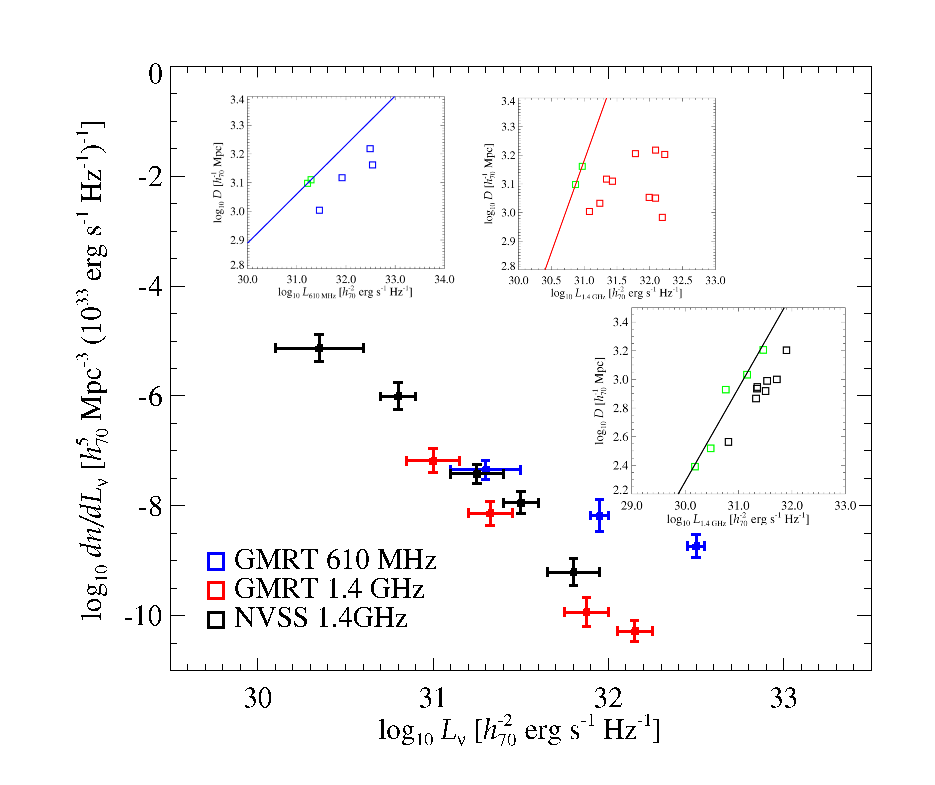
\includegraphics[width=0.48\textwidth]{figures/RLF_observations.eps}
\caption{RH luminosity function obtained from existent observations. The insets show the sample luminosity-distance distributions (see main text for details) where the solid line is the fit to the upper envelope population (indicated in green) employed to calculate the flux limit for the classical $V_{max}$ estimator. The choice of the upper envelope population is somehow arbitrary, particularly in the GMRT cases due to the poor luminosity--distance distributions. The horizontal error bars represent the mass bins while the vertical error bars are Poissonian uncertainties.}
\label{fig:RLFobs}
\end{figure}

\end{appendix}


%%%%%%%%%%%%%%%%%%%%%%%%%%%%%%%%%%%%%%%%%%%%%%%%%%%%%%%%%%%%%%%%%%
%%%%%%%%%%%%%%%%%%%%%%%%%%%%%%%%%%%%%%%%%%%%%%%%%%%%%%%%%%%%%%%%%%
\end{document}

%\del{In comparing with observations, we take as reference
%  \cite{2010MNRAS.406.1773M}. There are however many other works on this scaling
%  relation, in particularly we recall the HIghest X-ray FLUx Galaxy Cluster
%  Sample (HIFLUGCS; \citealp{2002ApJ...567..716R}), the REXCESS
%  \citep{2009A&A...498..361P} sample, and the 115 \emph{Chandra} cluster sample
%  of \cite{2007ApJ...668..772M}. The results on the slopes of the $L-M$ relation
%  can vary significantly between different samples. While the slope of
%  \cite{2010MNRAS.406.1773M} is $1.63\pm0.06$,
%  \cite{2002ApJ...567..716R}\footnote[8]{Note that we are quoting the
%    $L_{\rmn{bol}}-M_{200}$ results of \cite{2002ApJ...567..716R}.} found values
%  between $1.72\pm0.09$ and $1.89\pm0.08$ (depending on the fit procedure, which
%  also can affect the final result), \cite{2009A&A...498..361P} found
%  $2.08\pm0.13$ and \cite{2007ApJ...668..772M} found
%  $1.96\pm0.10$. Discrepancies can come from many different sources but likely
%  are to be charged to the selection criteria of the different samples as
%  recently pointed out also by \cite{2011arXiv1109.3708R}. Samples which differ
%  in e.g.~redshift distribution, mass range, fitting procedure and biases
%  treatment, and, of course, the used instrument, can give and actually gave
%  different results. Therefore we decided to take as reference the
%  \cite{2010MNRAS.406.1773M} work because it is very recent, their sample is
%  composed by a high number (238) of objects, and, more importantly, their
%  analysis takes self-consistently into account all selection effects,
%  covariances, systematic uncertainties and the cluster mass function (see also
%  \citealp{2010MNRAS.406.1759M}).}
